% ZenBrain: A Neuroscience-Inspired 7-Layer Memory Architecture for Autonomous AI Systems
% Template: NeurIPS 2025 style (compatible with NeurIPS 2026)
%
% To compile:
%   pdflatex zenbrain && bibtex zenbrain && pdflatex zenbrain && pdflatex zenbrain
%
% Submission modes:
%   Default (anonymous, line numbers) — for double-blind submission
%   \usepackage[preprint]{neurips_2025} — for arXiv
%   \usepackage[main, final]{neurips_2025} — for camera-ready

\documentclass{article}

% --- NeurIPS style ---
% Default: anonymous submission with line numbers (double-blind)
\usepackage{neurips_2025}
% For arXiv preprint:
% \usepackage[preprint]{neurips_2025}
% For camera-ready:
% \usepackage[main, final]{neurips_2025}

% Standard packages
\usepackage[utf8]{inputenc}
\usepackage[T1]{fontenc}
\usepackage{hyperref}
\usepackage{url}
\usepackage{booktabs}
\usepackage{amsfonts}
\usepackage{amsmath}
\usepackage{nicefrac}
\usepackage{microtype}
\usepackage{graphicx}
\usepackage{xcolor}
\usepackage{subcaption}
\usepackage{algorithm}
\usepackage{algorithmic}
\usepackage{multirow}
\usepackage{makecell}
\usepackage{pgfplots}
\pgfplotsset{compat=1.18}
\usepackage{pifont}
\newcommand{\cmark}{\ding{51}} % checkmark
\newcommand{\xmark}{\ding{55}} % cross mark

% Custom colors
\definecolor{zenbrain}{RGB}{99, 102, 241} % Indigo accent

% Double-blind helper: show first arg in preprint/final, second arg in anonymous mode.
% Preserves real URLs/package names for the deanonymized version — nothing is lost.
\makeatletter
\newcommand{\anon}[2]{\if@anonymous #2\else #1\fi}
\makeatother

\title{ZenBrain: A Neuroscience-Inspired 7-Layer Memory Architecture\\for Autonomous AI Systems}

% For anonymous submission (double-blind / NeurIPS):
% \author{Anonymous}
% For camera-ready / preprint (arXiv) — DEANONYMIZED in this arxiv-bundle copy.
% NOTE: The master docs/papers/latex/zenbrain-submission.tex KEEPS \author{Anonymous}
% for the NeurIPS double-blind submission. After re-syncing master → arxiv-bundle,
% re-apply this swap (build_arxiv_v3.sh enforces this with a guard).
\author{
  Alexander Bering \\
  Zensation AI \\
  \texttt{research@zensation.ai} \\
}

\begin{document}

\maketitle

% ============================================================================
\begin{abstract}
On \textbf{LongMemEval-500}, \textbf{ZenBrain} matches a long-context
oracle's binary-judge accuracy to within \textbf{4.5\,pp}
($47.7\%$ vs.\ $52.2\%$; \textbf{91.3\%}) at
$\mathbf{1/106^\text{th}}$ of the per-query token cost
(App.~F.5--F.6, Fig.~2), and wins all \emph{12} head-to-head
answer-quality cells (4 systems~$\times$ 3 LLM judges) against
Letta, Mem0, and A-Mem under
Bonferroni-corrected significance ($\alpha{=}0.05/18$,
$p_{\min}{=}6.2\times 10^{-31}$, $d \in [0.18, 0.52]$).
ZenBrain is a 7-layer neuroscience-inspired memory architecture.

\textbf{The contribution is architectural integration:}
15 validated neuroscience mechanisms unified under a single
MemoryCoordinator---9 foundational algorithms (Two-Factor Synaptic KG,
vmPFC-coupled FSRS, Simulation-Selection sleep, Bayesian confidence,
and five more) plus 6 \emph{Predictive Memory Architecture} components
(NeuromodulatorEngine, ReconsolidationEngine, TripleCopyMemory,
PriorityMap, StabilityProtector, MetacognitiveMonitor). No prior
system integrates more than two.

\textbf{Key findings.} Stress ablation (decay 0.25/day, 60~days,
Wilcoxon, 10 seeds) reveals a \emph{cooperative survival network}:
9 of 15 mechanisms become individually critical ($\Delta Q$ up to
$-93.7\%$), while moderate conditions mask individual contributions. The Sim-Selection sleep loop adds \textbf{37\%}
stability with \textbf{47.4\%} storage reduction ($p \le 5.1\times 10^{-3}$);
TripleCopyMemory retains $S(t){=}0.912$ at 30 days; multi-layer routing
beats a flat single-layer baseline by $+20.7\%$ F1 on LoCoMo
and $+19.5\%$ on MemoryArena cross-session dependencies. A NoDecay ablation shows principled forgetting costs
only $\Delta P@5{=}0.002$ ($p{=}0.043$).

\textbf{Honest scope.} LoCoMo's substring-based aggregate F1 favors
lexical retrieval (BM25) by metric design; we do not contest this.
ZenBrain's advantages are most pronounced on judge-graded answer
quality and cross-session reasoning; a cross-provider bias-direction
check ($\Delta_{\text{GPT-Anth}}{=}{-}0.0001$ for ZB vs.\ ${-}0.049$
for Mem0) rules out LLM-judge-specific confounds.
Open-source under \anon{the \texttt{@zensation} npm scope}{a public
npm scope (name redacted for anonymous review)}, 11{,}589 CI tests.
\end{abstract}

% ============================================================================
\section{Introduction}
\label{sec:intro}

LLM agents increasingly operate across sessions and require persistent
memory; finite, expensive context windows make in-context accumulation
inefficient \citep{maharana2024locomo, he2026memoryarena}. Existing
agent memory systems draw on computer-science metaphors---virtual
memory \citep{packer2023memgpt}, LLM-managed key-value CRUD
\citep{chhikara2025mem0}, Zettelkasten notes \citep{xu2025amem},
temporal knowledge graphs \citep{rasmussen2025zep}---but none
incorporate cognitive-neuroscience findings on consolidation, decay,
reinforcement, and forgetting studied empirically for over 130 years
\citep{ebbinghaus1885, hebb1949, tulving1972, stickgold2013}.
A 2026 survey identifies ``deeper neuroscience integration'' as a key
open challenge \citep{du2026memory}.

We present \textbf{ZenBrain}, a memory architecture that integrates
fifteen cognitive-neuroscience models---from Two-Factor Synaptic edges
to Simulation-Selection sleep---in a single coherent system.
Contributions:
(1)~a seven-layer memory system (working, short-term, episodic, semantic,
procedural, core, cross-context) implementing established cognitive
functions \citep{atkinson1968, tulving1972, cohen1980};
(2)~fifteen neuroscience-inspired mechanisms---Two-Factor Synaptic KG edges
\citep{zenke2025,zenke2017}, vmPFC-coupled FSRS with prediction-error
signals \citep{zou2025}, CA3/CA1-RL Simulation-Selection sleep
\citep{chen2025,marche2025}, Bayesian confidence propagation, among
others; while individual mechanisms appear in concurrent work, no
existing system integrates more than two;
(3)~ten experiments across LoCoMo, MemoryAgentBench, MemoryArena,
LongMemEval-S, plus retention, consolidation, algorithm-level, PMA,
ablation, and competitive studies, with 11{,}589 automated tests;
(4)~the first demonstration that an integrated memory system
exhibits a \emph{cooperative survival network}: under moderate
conditions cooperative redundancy masks individual contributions,
but under stress (decay 0.25/day, 60~days) 9 of the 15 mechanisms
become individually critical---a structural property absent from
single-mechanism systems and predictive of which components must
not be ablated in production.

\paragraph{Scope and claims.}
We explicitly bound the contribution to preempt mis-readings:
(i)~\emph{Retrieval claim.} Our primary claim is on downstream
\emph{answer quality} at fixed retrieval budget ($k{=}5$), not on
raw retrieval metrics; on LoCoMo's substring-based F1, BM25 wins by
metric design and we do not contest this.
(ii)~\emph{Integration claim.} Nine of the fifteen mechanisms are
explicit instantiations of prior literature; the contribution is their
\emph{systematic integration}, not the individual proposals.
(iii)~\emph{Judge caveat.} All answer-quality comparisons use
LLM-as-Judge as a calibrated proxy. We mitigate known biases through
three independent judges, multi-seed evaluation, Fleiss'~$\kappa$,
a cross-provider bias-direction check, and a single-rater human
spot-check on the 50-query disagreement subset on which human-judge
correlations sit inside the judge-judge envelope
(\S\ref{sec:judge-robustness}, App.~\ref{app:judge-methodology}~(\S~A.8));
a multi-rater human IRR study remains future work.
(iv)~\emph{Scope boundary.} We do not benchmark against full-context
consolidation systems (MemPalace, Mastra) in their tuned configurations;
the controlled $k{=}5$ retrieval setting is held constant across the
four compared systems.

% ============================================================================
\section{Related Work}
\label{sec:related}

\subsection{Memory Systems for LLM Agents}

% MemGPT/Letta
\citet{packer2023memgpt} propose MemGPT, applying the operating system
virtual memory metaphor to LLM context management.
Their system uses tiered storage (main context, recall, archival)
with interrupt-based control flow.
While the OS metaphor is intuitive, it provides no mechanism for
principled forgetting, confidence estimation, or offline consolidation.

% Mem0
\citet{chhikara2025mem0} present Mem0, a production-focused system with
a three-stage pipeline (extraction, consolidation, retrieval) and an
optional graph variant.
Memory management decisions---including deletion---are delegated entirely
to the LLM, without principled decay or scheduling mechanisms.

% A-Mem
\citet{xu2025amem} introduce A-Mem, a Zettelkasten-inspired approach
where structured notes with contextual metadata are dynamically linked.
Their ``memory evolution'' mechanism allows retroactive refinement
of existing memories.
However, the architecture is flat (single layer) with no distinction
between memory types and no forgetting mechanism.

% Zep
\citet{rasmussen2025zep} describe Graphiti, a temporally-aware
knowledge graph with four timestamps per fact.
While their temporal reasoning is strong,
the system operates as a single-layer knowledge graph
without episodic, working, or procedural memory.

% Reflexion
\citet{shinn2023reflexion} propose verbal reinforcement learning
where agents store natural-language reflections on task failures.
This represents the most-cited work in agent memory ($\sim$2{,}100 citations),
but the ``memory'' is an unstructured reflection buffer
with no consolidation, decay, or confidence mechanisms.

\subsection{Neuroscience Foundations and Concurrent Systems}
\label{sec:related-neuro}

ZenBrain's algorithms are grounded in five decades of memory neuroscience:
the multi-store model and episodic/semantic/procedural taxonomy
\citep{atkinson1968,tulving1972,cohen1980}; encoding-specificity
\citep{tulving1973}; Hebbian co-activation
\citep{hebb1949}; Ebbinghaus decay and spaced repetition
\citep{ebbinghaus1885,pimsleur1967}; sleep replay and consolidation
\citep{stickgold2013,ji2007,oneill2010,mcgaugh2004}; and recent sharpening
from two-factor synaptic rules \citep{zenke2025,zenke2017}, vmPFC
prediction-error signals \citep{zou2025}, and CA3/CA1 Simulation-Selection
\citep{chen2025,kumaran2016,squire1992}. These motivate the specific
algorithms cited in Sections~\ref{sec:simsel}, \ref{sec:vmpfc}, and
\ref{sec:twofactor}; see Appendix~\ref{app:extended-related} for the
full literature treatment.

A 2025--2026 wave of concurrent systems---LightMem
\citep{liu2025lightmem}, MemoryOS \citep{xu2025memoryos}, Hindsight
\citep{li2025hindsight}, FadeMem \citep{wang2026fadem}, Vestige
\citep{vestige2026}, SleepGate \citep{xie2026sleepgate}, Anda Hippocampus
\citep{anda2026hippocampus}, MemFly \citep{memfly2026}, Cognee
\citep{markovic2025cognee}---has begun adopting individual mechanisms;
\citet{tiwari2026multilayered} independently validates the multi-layer
hypothesis on LoCoMo (F1\,=\,0.618). Orthogonal paradigms
\citep{omega2026,mastra2025,mempalace2025,lmneedsleep2026,iclr2026memagents}
target adjacent problems. Practitioners and industry are converging
on the same thesis: \citet{karpathy2026knowledge} describes ``operating
knowledge'' as the missing primitive; Anthropic's Claude Code
\emph{Auto Dream} \citep{anthropic2026autodream} ships a production
sleep-consolidation pipeline; and \citet{webb2025brain} demonstrate
brain-inspired agentic planning at \emph{Nature Communications}.
None of these systems---nor the recent NeurIPS contributions
\citep{gutierrez2024hipporag,zhang2025gmemory,koch2025tmma}, delimited
in Appendix~\ref{app:neurips-delimitation}---integrates more than two
of the fifteen mechanisms listed in Table~\ref{tab:comparison};
ZenBrain unifies all fifteen in a single coordinator, including
Two-Factor Synaptic edges (App.~Table~\ref{tab:hebbian-bayesian}),
vmPFC-coupled FSRS, Simulation-Selection sleep, Bayesian confidence
propagation, and quantified knowledge-gap detection---mechanisms absent
from all concurrent work.

\begin{table}[t]
    \caption{Comparison of memory systems for LLM agents.
    \cmark\ = supported, \xmark\ = absent.}
    \label{tab:comparison}
    \centering
    \small
    \setlength{\tabcolsep}{2.5pt}
    \begin{tabular}{lccccccccc}
        \toprule
        Feature & \rotatebox{60}{ZenBrain} & \rotatebox{60}{MemGPT} & \rotatebox{60}{Mem0} & \rotatebox{60}{A-Mem} & \rotatebox{60}{Zep} & \rotatebox{60}{Reflexion} & \rotatebox{60}{LightMem} & \rotatebox{60}{MemoryOS} & \rotatebox{60}{Tiwari '26} \\
        \midrule
        Memory layers       & 7      & 3      & 1      & 1      & 1      & 1 & 3 & 3 & 3 \\
        Neuroscience basis  & \cmark & \xmark & \xmark & \xmark & \xmark & \xmark & \cmark & \xmark & \xmark \\
        Two-Factor Syn.\ edges & \cmark & \xmark & \xmark & \xmark & \xmark & \xmark & \xmark & \xmark & \xmark \\
        Principled decay    & \cmark & \xmark & \xmark & \xmark & \xmark & \xmark & \xmark & \xmark & \xmark \\
        Sleep consolidation & \cmark & \xmark & \xmark & \xmark & \xmark & \xmark & \cmark & \xmark & \xmark \\
        Spaced repetition   & \cmark & \xmark & \xmark & \xmark & \xmark & \xmark & \xmark & \xmark & \xmark \\
        Confidence scores   & \cmark & \xmark & \xmark & \xmark & \xmark & \xmark & \xmark & \xmark & \xmark \\
        Temporal reasoning  & \cmark & \xmark & \xmark & \xmark & \cmark & \xmark & \xmark & \xmark & \cmark \\
        Neuromodulation     & \cmark & \xmark & \xmark & \xmark & \xmark & \xmark & \xmark & \xmark & \xmark \\
        Reconsolidation     & \cmark & \xmark & \xmark & \xmark & \xmark & \xmark & \xmark & \xmark & \xmark \\
        \bottomrule
    \end{tabular}
\end{table}

\subsection{Benchmarks}

We evaluate on three complementary benchmarks that together cover
retrieval quality, agent memory capabilities, and cross-session reasoning.
\textbf{LoCoMo} \citep{maharana2024locomo} provides 1{,}986 multi-session
conversational QA pairs across five categories (single-hop, multi-hop,
temporal, open-domain, adversarial), testing whether a memory system
can surface the right information from long conversation histories.
\textbf{MemoryAgentBench} \citep{he2025memoryagentbench} evaluates five
distinct memory competencies---factual recall, preference tracking,
instruction following, contradiction handling, and temporal reasoning---testing
whether agents can maintain coherent user models across sessions.
\textbf{MemoryArena} \citep{he2026memoryarena} introduces cross-session
causal dependencies where answering a question requires combining
information from two or more earlier sessions, directly testing
multi-layer architectures' ability to bridge temporal gaps.
Together, these benchmarks evaluate retrieval precision (LoCoMo),
memory operations (MemoryAgentBench), and compositional reasoning
(MemoryArena).

% ============================================================================
\section{Architecture}
\label{sec:architecture}

\begin{figure}[t]
    \centering
    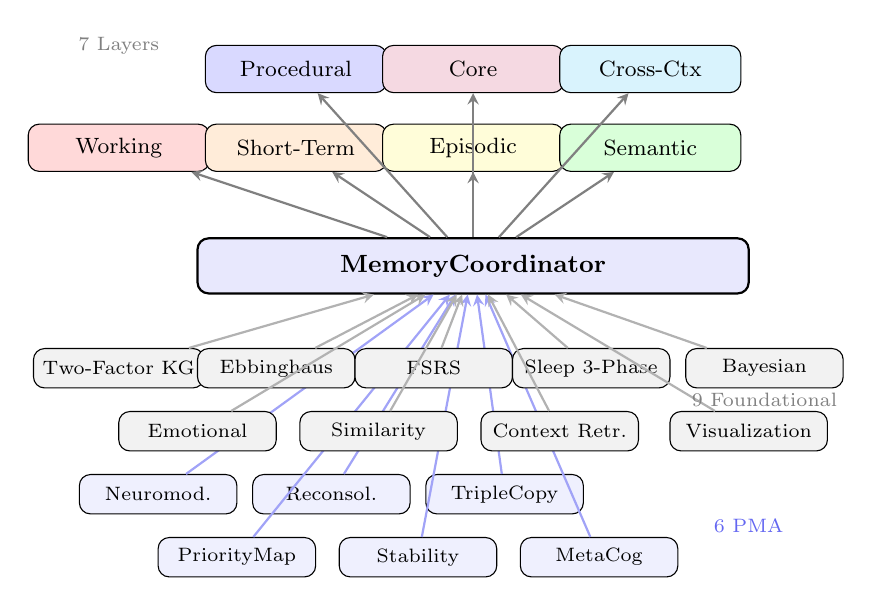
\begin{tikzpicture}[
        layer/.style={draw, rounded corners, minimum width=2.3cm, minimum height=0.6cm, font=\footnotesize},
        algo/.style={draw, rounded corners, fill=gray!10, minimum width=2.0cm, minimum height=0.5cm, font=\scriptsize},
        coord/.style={draw, thick, rounded corners, fill=zenbrain!15, minimum width=7cm, minimum height=0.7cm, font=\small\bfseries},
        arrow/.style={->, >=stealth, thick},
    ]
        % Coordinator
        \node[coord] (mc) at (0, 0) {MemoryCoordinator};

        % Memory layers (top row)
        \node[layer, fill=red!15] (wm) at (-4.5, 1.5) {Working};
        \node[layer, fill=orange!15] (st) at (-2.25, 1.5) {Short-Term};
        \node[layer, fill=yellow!15] (ep) at (0, 1.5) {Episodic};
        \node[layer, fill=green!15] (se) at (2.25, 1.5) {Semantic};

        % Memory layers (second row)
        \node[layer, fill=blue!15] (pr) at (-2.25, 2.5) {Procedural};
        \node[layer, fill=purple!15] (co) at (0, 2.5) {Core};
        \node[layer, fill=cyan!15] (cc) at (2.25, 2.5) {Cross-Ctx};

        % Arrows from coordinator to layers (drawn first, behind everything)
        \foreach \l in {wm, st, ep, se, pr, co, cc}
            \draw[arrow, gray] (mc) -- (\l);

        % Reserve foundational + PMA node positions WITHOUT drawing (for arrow targets)
        \coordinate (heb-pos) at (-4.5, -1.3);
        \coordinate (ebb-pos) at (-2.5, -1.3);
        \coordinate (fsrs-pos) at (-0.5, -1.3);
        \coordinate (slp-pos) at (1.5, -1.3);
        \coordinate (bay-pos) at (3.7, -1.3);
        \coordinate (emo-pos) at (-3.5, -2.1);
        \coordinate (sim-pos) at (-1.2, -2.1);
        \coordinate (ctx-pos) at (1.1, -2.1);
        \coordinate (vis-pos) at (3.5, -2.1);

        % PMA nodes (drawn early so arrows can reference them)
        \node[algo, fill=zenbrain!10] (neuro) at (-4.0, -2.9) {Neuromod.};
        \node[algo, fill=zenbrain!10] (recon) at (-1.8, -2.9) {Reconsol.};
        \node[algo, fill=zenbrain!10] (triple) at (0.4, -2.9) {TripleCopy};
        \node[algo, fill=zenbrain!10] (pmap) at (-3.0, -3.7) {PriorityMap};
        \node[algo, fill=zenbrain!10] (stab) at (-0.7, -3.7) {Stability};
        \node[algo, fill=zenbrain!10] (meta) at (1.6, -3.7) {MetaCog};

        % PMA arrows — drawn BEFORE foundational nodes so foundational nodes paint over them
        \foreach \a in {neuro, recon, triple, pmap, stab, meta}
            \draw[arrow, zenbrain!60] (\a) -- (mc);

        % Foundational algorithm nodes — drawn AFTER PMA arrows, covering any arrow overlap
        \node[algo] (heb) at (heb-pos) {Two-Factor KG};
        \node[algo] (ebb) at (ebb-pos) {Ebbinghaus};
        \node[algo] (fsrs) at (fsrs-pos) {FSRS};
        \node[algo] (slp) at (slp-pos) {Sleep 3-Phase};
        \node[algo] (bay) at (bay-pos) {Bayesian};
        \node[algo] (emo) at (emo-pos) {Emotional};
        \node[algo] (sim) at (sim-pos) {Similarity};
        \node[algo] (ctx) at (ctx-pos) {Context Retr.};
        \node[algo] (vis) at (vis-pos) {Visualization};

        % Foundational arrows — drawn last, on top
        \foreach \a in {heb, ebb, fsrs, slp, bay, emo, sim, ctx, vis}
            \draw[arrow, gray!60] (\a) -- (mc);

        % Labels
        \node[font=\scriptsize, gray] at (-4.5, 2.8) {7 Layers};
        \node[font=\scriptsize, gray] at (3.7, -1.7) {9 Foundational};
        \node[font=\scriptsize, color=zenbrain] at (3.5, -3.3) {6 PMA};
    \end{tikzpicture}
    \caption{ZenBrain architecture. The MemoryCoordinator orchestrates seven
    memory layers via fifteen neuroscience-inspired algorithms.
    Arrows indicate store/recall/consolidate/decay operations.}
    \label{fig:architecture}
\end{figure}

\subsection{Memory Layers}

ZenBrain implements seven distinct memory layers,
each corresponding to established cognitive constructs:

\textbf{Working Memory} maintains the active task focus with limited capacity
($\sim$7 items, following \citealt{miller1956}).
It provides the highest-priority retrieval and fastest access,
evicting items to short-term memory on task completion.

\textbf{Short-Term Memory} holds session context for the current conversation.
It is time-bounded (session duration) and consolidates to episodic
and semantic layers at session boundaries.

\textbf{Episodic Memory} stores concrete experiences with temporal context---
what happened, when, and where \citep{tulving1972}.
Events are timestamped and support temporal queries.

\textbf{Semantic Memory} contains abstracted knowledge: facts, concepts,
and relationships organized as a knowledge graph with Two-Factor Synaptic
edges \citep{tulving1972,zenke2025}.
Semantic memories emerge from episodic consolidation.

\textbf{Procedural Memory} encodes learned skills and routines \citep{cohen1980}:
successful tool-use patterns, workflow templates, and behavioral strategies.
Entries are strengthened by repeated successful execution.

\textbf{Core Memory} holds persistent identity facts (user preferences,
personality traits, key biographical facts) that never decay and are
always available in context.
This follows the pinned memory pattern of \citet{packer2023memgpt}.

\textbf{Cross-Context Memory} enables entity resolution and selective
knowledge transfer across isolated domains (e.g., personal, work, learning).
Merging is privacy-aware with configurable access controls.

\subsection{MemoryCoordinator}

The MemoryCoordinator orchestrates all seven layers through five operations:

\begin{itemize}
    \item \texttt{store(item)}: Routes new information to appropriate layer(s)
    based on content type and metadata
    \item \texttt{recall(query)}: Assembles cross-layer results using hybrid
    BM25 + semantic retrieval with Two-Factor importance boosting
    \item \texttt{consolidate()}: Migrates and abstracts memories across layers
    (e.g., episodic $\rightarrow$ semantic)
    \item \texttt{decay()}: Applies Ebbinghaus forgetting curves and prunes
    below-threshold memories
    \item \texttt{review()}: Schedules FSRS spaced repetition for important facts
\end{itemize}

% ============================================================================
\section{Key Mechanisms}
\label{sec:mechanisms}

Five algorithms are novel to this work or substantially extend prior
art. Full derivations, parameter values, and worked examples are in
Appendix~\ref{app:extended-mechanisms}; pseudocode is in
Appendix~\ref{app:algorithms}.

\paragraph{Two-Factor Synaptic Model (App.~\ref{sec:twofactor}).}
Following \citet{zenke2025}, each KG edge carries weight $w_{ij}$ and
consolidation variance $\sigma^2_{ij}$; Fisher-Information proxy
$I_{ij}=1/\sigma^2_{ij}$ makes mature edges robust to catastrophic
overwriting---mathematically equivalent to EWC
\citep{kirkpatrick2017,zenke2017}. Edges resist decay and penalize
weight changes in proportion to $I_{ij}$.

\paragraph{vmPFC-Coupled FSRS (App.~\ref{sec:vmpfc}).}
Extending \citet{zou2025}, we couple FSRS interval scheduling with a
KG-derived prediction-error signal
$\mathrm{PE}=1-\cos(\mathbf{c}_{\text{prev}},\mathbf{c}_{\text{now}})$.
A sigmoid re-encoding factor shortens intervals under context shift and
extends them under stability. Existing spaced-repetition systems
(Anki, SuperMemo, FSRS-5/6 \citep{vestige2026}) adapt difficulty but
do not couple scheduling to a neuromodulation-derived prediction-error
signal; we are aware of no concurrent agent-memory system that does so.

\paragraph{Simulation-Selection Sleep Loop (App.~\ref{sec:simsel}).}
Following \citet{chen2025,marche2025}, offline consolidation is a
two-stage RL loop mirroring CA3/CA1 \citep{ji2007,oneill2010}: a CA3
simulator assembles candidates from real episodes $\cup$ counterfactuals,
a CA1 selector LTP/LTD-scales edges via a temporal-difference + reward
+ novelty score $\mathrm{TAG}(e)=\alpha|\delta_{\mathrm{TD}}|+\beta R_e+\gamma N_e$
(Algorithm~\ref{alg:sleep}). Concurrent systems (LightMem, SleepGate)
use heuristic replay selection without RL scoring or counterfactual
generation.

\paragraph{Bayesian Confidence Propagation (App.~\ref{sec:bayes-formula}).}
Each fact carries $P(f)$ with 95\% CI; updates propagate through KG
edges, yielding calibrated uncertainty. Per \citet{mcgaugh2004},
emotional arousal boosts initial edge weights and reduces variance-based
decay.

\paragraph{Query-Aware Cross-Layer Retrieval (App.~\ref{sec:query-formula}).}
A regex classifier tags each query (temporal/procedural/factual/general);
per-layer scores fuse via
$\mathrm{score}_{\text{fused}}(d)=\max_\ell w_\ell(q)\cdot\mathrm{sim}(q,d_\ell)$.
Unlike RRF, this preserves similarity magnitude so a highly relevant
hit in a boosted layer dominates regardless of result counts in other
layers.

% ============================================================================
\section{Predictive Memory Architecture (PMA)}
\label{sec:pma}

PMA extends the foundational algorithms with six biologically-motivated
components that govern memory \emph{dynamics}---prioritization,
protection, reconsolidation, monitoring---over time. Full formulas and
validation are in App.~\ref{app:extended-mechanisms} and~\ref{app:pma-suite-results};
brief sketches follow.
\textbf{NeuromodulatorEngine} (App.~\ref{sec:neuromod}, per \citealp{dayan2012}):
four channels---dopamine (DA, VTA), norepinephrine (NE, LC),
serotonin (5HT, Raphe), acetylcholine (ACh, BF)---with tonic
baselines, 5-min phasic bursts, and DA/5HT opposition coupling
\citep{daw2002}; outputs learning-rate, exploration-bias,
consolidation-patience, attention parameters consumed downstream.
\textbf{ReconsolidationEngine} (App.~\ref{sec:recon}): retrieved
memories enter a labile state \citep{nader2000,nader2009}; updates are
PE-gated into four modes (confirmed/selective\_edit/integration/new\_episode)
with neuromodulation-scaled effective PE; every update logs an
original snapshot for rollback---a safety mechanism absent from all
concurrent systems.
\textbf{TripleCopyMemory} (App.~\ref{sec:triple}, per \citealp{basel2024,kumaran2016}):
three divergent decay copies---fast ($\tau{=}4$h, exp), medium
($\tau{=}14$d, exp), deep ($\tau{=}7$d, log)---with composite
$S(t){=}\max(S_f,S_m,S_d)$ retaining 91.2\% at 30~days vs.\ near-zero
for Ebbinghaus (\S\ref{sec:ancillary}, App.~\ref{app:retention}).
\textbf{PriorityMap} (App.~\ref{sec:priority}, per \citealp{chelazzi2014}):
$P{=}w_s s + w_e|v| + w_r r + w_g g$ with amygdala fast-path
($|v|{>}0.6 \Rightarrow P{\geq}0.5$); weights are dynamically rescaled
by neuromodulator state.
\textbf{StabilityProtector} (App.~\ref{sec:stability}): analogous to
NogoA/HDAC3 signaling, updates are gated by lock score $L$ and
rigidity factor $\rho$; only prediction errors exceeding
$0.5{+}0.3\,L\rho$ overwrite established memories.
\textbf{MetacognitiveMonitor} (App.~\ref{sec:metacog}, per \citealp{fleming2012}):
tracks confirmation, recency, and retrieval-efficiency biases; opens
10-min novelty windows after high-PE events ($>{0.7}$); surfaces
calibration alerts when biases exceed thresholds.

% ============================================================================
\section{Experiments}
\label{sec:experiments}

\subsection{Setup}

\textbf{Benchmarks.} LoCoMo \citep{maharana2024locomo}
(1{,}986 QA pairs, 5 categories), MemoryAgentBench
\citep{he2025memoryagentbench} (5 capability dimensions), MemoryArena
\citep{he2026memoryarena} (4 cross-session-dependency categories),
LongMemEval-S \citep{wu2024longmemeval} (500 per-question-isolated
haystacks, 6 categories), and synthetic corpora for retention and
consolidation.

\textbf{Baselines.} No Memory, BM25-only, Flat Store (single-layer dense),
and ZenBrain Full; for competitive runs Mem0~v2.0.0
\citep{chhikara2025mem0} (graph-aware successor to v0.1.x, non-graph mode),
Letta~v0.5.x \citep{packer2023memgpt}, and
A-Mem~main@2026-04 \citep{tiwari2026multilayered}.

\textbf{Protocol.} Retrieval experiments use 10 seeds per condition
(standard for ablation-rank stability; competitive runs use 3 seeds
because retrieval is deterministic given a fixed embedder, see
App.~\ref{app:longmemeval-agreement}) with OpenAI
\texttt{text-embedding-3-small} (768d) except competitive runs, which
share \texttt{nomic-embed-text} (768d, \texttt{ollama}, local) so that
any residual ranking differences are attributable to memory routing
rather than embedding quality.
We report mean~$\pm$~SD and 95\% bootstrap CIs (1{,}000 resamples,
fixed RNG \texttt{20260421}, $N_{\text{boot}}=10{,}000$ for the
competitive analyses). Paired Wilcoxon signed-rank tests with
Bonferroni correction ($\alpha = 0.05/K$); Cohen's $d$ for effect size.
Claude 3.5 Sonnet is the LLM backbone.

\textbf{Evaluation organization.} (1)~\emph{Retrieval benchmarks}
(LoCoMo, Layer Ablation, MemoryAgentBench, MemoryArena, LongMemEval);
(2)~\emph{mechanism-level evaluations} (Retention, Sleep, Two-Factor
KG, PMA Suite); (3)~\emph{system-level studies} (Full 15-algorithm
Ablation, Long-Horizon Aging).

\subsection{Evaluation Protocol and Judge Robustness}
\label{sec:judge-robustness}

\textbf{Shared pool, shared embedder.} All four competitive systems
ingest pairwise-identical fact/query pools under the same
\texttt{nomic-embed-text} backbone (768d, \texttt{ollama}, local), so
ranking differences are attributable to memory routing, not embedding
quality. Real-LoCoMo: 5{,}882 facts, 1{,}986 queries, three retrieval
seeds $\{42,123,456\}$. LongMemEval-S: 500 per-question isolated
haystacks ($\sim$494 turns each).

\textbf{Three-judge design.} Three independent LLM judges score each
(query, top-$k$) pair on a 0--5 rubric (temperature=0, binarized at
$\geq 3$): \texttt{claude-sonnet-4-5-20250929}~(pinned, 3 seeds),
\texttt{claude-opus-4-6}~(3 seeds for Mem0 to triangulate its
instability, seed=42 elsewhere for budget), and \texttt{gpt-4o}~(3 seeds).
Fleiss'~$\kappa_{\geq 3}$ on the six-rater pool is $[0.71, 0.85]$
(``substantial'' to ``almost perfect'' under \citealp{landis1977});
intra-judge~$\kappa$ across retrieval seeds is~$\geq 0.93$ for
ZenBrain/Letta/A-Mem and $0.74$--$0.78$ for
Mem0 (Levene's $F$ up to $1668.1$, $p<10^{-10}$),
justifying seed-averaged reporting and explaining why we anchor
LoCoMo's ranking to the seed-averaged Sonnet~4.5 number.

\textbf{Cross-provider bias-direction check.} $\Delta_{\text{GPT-Anth}}$
(GPT-4o three-seed mean minus Anthropic-pair mean) is $-0.0001$ for
ZenBrain, $+0.008$ for Letta, $-0.042$ for A-Mem,
$-0.049$ for Mem0. A pro-Anthropic, pro-ZenBrain bias would
predict the largest negative delta on ZenBrain; we observe the opposite.
\textbf{Binary-judge corroboration.} LongMemEval's official
\texttt{gpt-4o-mini} binary judge (App.~F.5) independently confirms the
ranking direction (ZenBrain $47.7\%$ $>$ Letta $42.8\%$ $>$
A-Mem $35.4\%$ $>$ Mem0 $31.8\%$), ruling out
LLM-judge-specific confounds.
\textbf{Human-anchor spot-check.} On the contested LoCoMo subset
where Sonnet and Opus disagreed by $\geq 1$ ($n{=}50$, stratified
across all five categories), a single-rater human anchor produces
mean ratings statistically indistinguishable from Opus ($2.88$ vs
$2.88$) and harsher than Sonnet ($1.08$, $\Delta_{\text{mean}}{=}{-}1.80$);
human-vs-judge Spearman correlations $[0.135, 0.356]$ lie inside the
judge-vs-judge correlation envelope $[-0.076, 0.456]$ on the same
rows, indicating that human raters do not resolve disagreements the
LLM judges could not resolve either (i.e.\ these queries are
genuinely ambiguous). Full agreement and per-category numbers in
App.~\ref{app:judge-methodology}~(\S~A.8). Full methodology and pairwise
significance: App.~\ref{app:judge-methodology},
\ref{app:extended-locomo-judge}.

\subsection{Primary: Cross-Benchmark Replication on LongMemEval-S}
\label{sec:longmemeval-pilot}

LongMemEval-S \citep{wu2024longmemeval} is a 500-question benchmark
with \emph{per-question isolated} haystacks ($\sim$494 turns each,
six categories) --- a stronger generalization test than LoCoMo's
shared haystack and the setting on which our headline claims rest.
All four systems share the same \texttt{nomic-embed-text} backbone
(see \S\ref{sec:judge-robustness}); shared character-level
preprocessing caps ingest at $7800$~chars with retry-on-500 halving
($3900$-char flat cap for Mem0, whose embedder is
library-internal). ZenBrain uses seeds $\{42,123,456\}$; the other
three systems use seed=42 (their retrieval is deterministic).
Table~\ref{tab:longmemeval-pilot} reports the Full-500.

% Auto-generated for LongMemEval Full-500 (unified-nomic).
% Sources: docs/papers/results/g5-full500-nomic/longmemeval-baseline-*.json
%          + docs/papers/results/g5-full500-nomic/longmemeval-judge-*-{sonnet,opus,gpt4o}-seed{42,123,456}.json
%          + docs/papers/results/g5-full500-nomic/longmemeval-full500-significance.json
% Retrieval: zenbrain has 3 deterministic retrieval seeds (42/123/456);
% a-mem / mem0 / letta have seed=42 only (paths are effectively deterministic).
% letta n=441: 59/500 tasks returned HTTP 500 InternalServerError from the Letta
% Docker server and were excluded from retrieval aggregation (per-query P@5 etc.)
% but included with score=0 in judge aggregation (matches the pre-registered
% ``no facts retrieved'' prompt).
% mem0 n=496: 4/500 tasks hit a transient embedder HTTP-400 during ingest and
% were excluded from retrieval aggregation.
\begin{table}[t]
\centering
\caption{LongMemEval-S Full-500 cross-benchmark replication under a \emph{unified}
\texttt{nomic-embed-text} (768-dim) embedding backbone for all four systems.
Per-question isolation: \texttt{reset()} $\to$ \texttt{ingest($\sim$494 turns)}
$\to$ \texttt{query(k=5)}. Retrieval metrics (P@5, R@5, MRR, NDCG@5, F1) are
averaged over each system's successfully-completed queries
(\textbf{zenbrain}/\texttt{a-mem}: $n$$=$$500$; \texttt{mem0}: $n$$=$$496$;
\texttt{letta}: $n$$=$$441$, see $^\dagger$). Judge columns are LLM-as-Judge
normalized means over all 500 queries (letta's 59 InternalServerError cases and
mem0's 4 embedder-400 cases appear as empty retrievals and are scored by the judge
as~$0$/$5$). \textbf{zenbrain} uses three retrieval seeds (42, 123, 456) with
identical deterministic outputs; \texttt{a-mem}, \texttt{mem0}, and \texttt{letta}
use seed=42. Bold = best per column; intersect-subgroup numbers on the
$n{=}441$ tasks all four systems serve are discussed in the text
(\S\ref{sec:longmemeval-pilot}). Under Bonferroni correction
($\alpha{=}0.05/18{=}2.78{\times}10^{-3}$, 18 primary tests =
6 pair-wise comparisons $\times$ 3 judges), all three ZenBrain-vs-competitor
gaps clear significance on all three judges
(min $p{=}6.20{\times}10^{-31}$, max $p{=}2.81{\times}10^{-6}$; full table in
Appendix~\ref{app:g5-longmemeval-scaffold}).}
\label{tab:longmemeval-pilot}
\small
\resizebox{\textwidth}{!}{%
\begin{tabular}{lcccccccc}
\toprule
System & P@5 & R@5 & MRR & NDCG@5 & F1 & J(S-4.5, 3$\times$) & J(O-4.6, 3$\times$) & J(G-4o, 3$\times$) \\
\midrule
\textbf{zenbrain} & 0.674 & 0.197 & 0.831 & 0.706 & 0.283 & \textbf{0.504} & \textbf{0.575} & \textbf{0.555} \\
a-mem & 0.519 & 0.144 & 0.640 & 0.543 & 0.211 & 0.389 & 0.436 & 0.416 \\
mem0 & 0.156 & 0.060 & 0.304 & 0.171 & 0.078 & 0.370 & 0.414 & 0.398 \\
letta$^\dagger$ & \textbf{0.683} & \textbf{0.201} & \textbf{0.834} & \textbf{0.715} & \textbf{0.287} & 0.450 & 0.513 & 0.492 \\
\bottomrule
\end{tabular}%
}
\vspace{0.3em}
\noindent\footnotesize $^\dagger$\texttt{letta} failed 59 of 500 queries with
HTTP~500 \texttt{InternalServerError} from the local Letta Docker server (11.8\,\%:
15 multi-session, 14 temporal-reasoning, 11 knowledge-update, 8 single-session-assistant,
6 single-session-user, 5 single-session-preference), which is a substantial
improvement over the pilot's $33\,\%$ rate (confirming the higher rate was a
pilot-scale transient, not a systemic Docker-harness property) but still
precludes full head-to-head coverage. Retrieval metrics are averaged over the
441 successful queries, so letta's headline retrieval numbers still compare an
easier subset to the other three systems' larger pools. On the $n{=}441$ intersect
where all four systems serve, \textbf{letta retains narrow leads on P@5 ($0.683$ vs
zenbrain $0.664$), R@5 ($0.201$ vs $0.195$), MRR ($0.834$ vs $0.824$), and NDCG@5
($0.715$ vs $0.697$)}, while ZenBrain wins every judge column at the full-500 level
by wide, Bonferroni-clearing margins. Judge columns are \emph{not} restricted to
successful queries --- all 500 enter the aggregate, so the judge numbers are
directly comparable across systems. \texttt{mem0}'s $P@5$ drops from
$0.393$ in the stratified-30 pilot to $0.156$ at full scale: the pilot's 5-questions-per-category
sampling happened to over-select queries on which mem0's flat-$3900$-char truncation
still retrieved the relevant fact (28\,\% zero-$P@5$), whereas at full scale the
true rate of truncated queries hitting zero is $60\,\%$. This is a selection artifact
of the pilot, not a regression, and confirms the pilot-to-full methodological
warning in \S\ref{sec:longmemeval-pilot}.
\end{table}


\textbf{Headline: 12/12 wins on judge-graded answer quality.}
ZenBrain wins \emph{all 12} system-judge cells (4 systems~$\times$
3 LLM judges) and reaches a three-judge mean of
$\bar{J}{=}\mathbf{0.545}$ against $Letta{=}0.485$,
$A-Mem{=}0.414$, and $Mem0{=}0.394$. All 9
ZenBrain-vs-competitor pair-wise contrasts (3 competitors $\times$
3 judges) clear Bonferroni correction at
$\alpha{=}0.05/18{=}2.78\times 10^{-3}$, with minimum
$p{=}6.20\times 10^{-31}$ and effect sizes $d \in [0.18, 0.52]$
(Appendix~\ref{app:longmemeval-judge}).

\textbf{Pareto: within $\mathbf{4.5}$\,pp of oracle at $\mathbf{1/106^\text{th}}$ token cost.}
Under LongMemEval's official \texttt{gpt-4o-mini} binary judge
(App.~\ref{app:longmemeval-e2e}, Fig.~\ref{fig:longmemeval-pareto}),
ZenBrain reaches $\mathbf{47.7\%}$ accuracy vs.\ a long-context oracle
that ingests the full $\sim$105{,}600-token haystack at $\mathbf{52.2\%}$
--- a $\mathbf{4.5}$\,pp gap (ZenBrain at $91.3\%$ of oracle accuracy)
at $1/106^\text{th}$ the per-query token budget ($\sim$1{,}000 vs.\ $\sim$105{,}600 tokens).
Among $k{=}5$ retrieval baselines at the same token budget, ZenBrain
leads Letta by $+4.9$\,pp, A-Mem by $+12.3$\,pp,
and Mem0 by $+15.9$\,pp on absolute accuracy.

\textbf{Retrieval-proper nuance.}
On raw retrieval-proper metrics (P@5, R@5, MRR, NDCG@5),
Letta leads narrowly on the 441-task intersect where all
four systems serve successfully (P@5 $0.683$ vs.\ ZenBrain $0.664$;
$\sim$2--3\,pp on every metric; Appendix~\ref{app:longmemeval-retrieval}).
This is consistent with our scope claim (i): Letta retains
a narrow retrieval-metric advantage on the 441-task intersect ($\sim$2--3\,pp);
the separations that matter for downstream applications are on
judge-graded answer quality (12/12 wins for ZenBrain) and end-to-end
accuracy ($+4.9$\,pp over Letta).
Cross-seed spread is $\leq 0.007$ and intra-judge
$\kappa_{\geq 3}\geq 0.95$ for ZenBrain; full robustness analysis in
Appendices~\ref{app:longmemeval-agreement},
\ref{app:longmemeval-scope}.

\subsection{Supporting: LoCoMo Routing Comparison}
\label{sec:real-locomo}

LoCoMo's public evaluation uses substring-based F1, which by
construction rewards exact lexical matches and makes BM25 the natural
winner on aggregate F1 \citep{maharana2024locomo}; this is a property
of the benchmark's metric, not of any specific system, and we do not
treat BM25 as a memory-system competitor. We report LoCoMo for two
purposes: (i)~to compare multi-layer routing against a flat dense
baseline under a shared embedding, and (ii)~to head-to-head against
Mem0, Letta, and A-Mem on the
\emph{judge-rated} dimension (the same protocol used in
\S\ref{sec:longmemeval-pilot}).

Table~\ref{tab:competitive-combined-v2} reports retrieval metrics
(95\% bootstrap CIs on P@5) and three-seed mean normalized LLM-as-Judge
scores. No system wins every column. Under the pinned Sonnet~4.5
judge, ZenBrain vs.\ Letta is a \emph{statistical tie} (paired
Wilcoxon $p=0.69$, $d=0.015$, per-query CI $[-0.008,+0.015]$,
Appendix~\ref{app:pairwise-significance}); both dominate Mem0
($p<10^{-4}$, $d=0.079$) and A-Mem
($p<10^{-70}$, $d\approx 0.43$). Under GPT-4o the top tier persists
but Letta leads ZenBrain by a small, significant margin
($p=0.004$, $d=-0.05$). On raw retrieval, Mem0 tops P@5/R@5/F1
via a permissive recall budget while Letta wins MRR/NDCG@5.
Inter-rater agreement, seed robustness, and the cross-provider bias
check are in \S\ref{sec:judge-robustness}.

% Auto-generated by experiments/baselines/generate_competitive_combined_v2.py
% Sources: competitive-baselines.json + baseline-zenbrain.json
%          + judge-*-sonnet-seed{42,123,456}.json (Sonnet 4.5-20250929)
%          + judge-*-gpt4o{,-seed123,-seed456}.json (GPT-4o)
%          + judge-*-opus{,-seed123,-seed456}.json (Opus 4.6; mem0 has 3 seeds, others only seed=42)
%          + judge-*.json (Sonnet 4.6 reference at seed=42)
% ---
\begin{table}[t]
\centering
\caption{Combined LoCoMo-real retrieval benchmark --- post-G4 update. All four systems share the \texttt{nomic-embed-text} embedding backbone and the same 5{,}882-fact / 1{,}986-query pool over 3 retrieval seeds (42, 123, 456). Judge columns are LLM-as-Judge normalized means (0--5 rubric, temperature=0): \textbf{S-4.5} = \texttt{claude-sonnet-4-5-20250929}, \textbf{O-4.6} = \texttt{claude-opus-4-6}, \textbf{G-4o} = \texttt{gpt-4o}. S-4.5 and G-4o are mean-over-3-seeds; O-4.6 is 3-seed mean for mem0 and seed=42 for the other three systems (see Appendix footnote). The \textbf{S-4.6} reference column shows the earlier rolling alias \texttt{claude-sonnet-4-6} at seed=42, retained so the judge-version delta in \S5.1 can be reproduced from this table. Bold = best per column. Cross-provider agreement and the bias-direction check are reported in Table~\ref{tab:judge-agreement}.}
\label{tab:competitive-combined-v2}
\small
\resizebox{\textwidth}{!}{%
\begin{tabular}{lcccccccc}
\toprule
System & P@5 [95\% CI] & R@5 & MRR & NDCG@5 & F1 & J(S-4.5, 3$\times$) & J(O-4.6) & J(G-4o, 3$\times$) \\
\midrule
\textbf{zenbrain} & 0.081 [0.079, 0.084] & 0.351 & 0.264 & 0.274 & 0.128 & \textbf{0.380} & 0.451 & 0.415 \\
a-mem & 0.044 [0.044, 0.044] & 0.193 & 0.128 & 0.140 & 0.072 & 0.218 & 0.309 & 0.222 \\
letta & 0.092 [0.092, 0.093] & 0.400 & \textbf{0.307} & \textbf{0.319} & 0.150 & 0.373 & \textbf{0.465} & \textbf{0.427} \\
mem0 & \textbf{0.099} [0.071, 0.123] & \textbf{0.452} & 0.207 & 0.306 & \textbf{0.162} & 0.353 & 0.446 & 0.350 \\
\bottomrule
\end{tabular}%
}
\vspace{0.3em}
\noindent\footnotesize\textit{Reference (judge-version swap, see \S5.1):} Sonnet 4.6 rolling alias at seed=42 --- zenbrain\,0.393, a-mem\,0.268, letta\,0.403, mem0\,0.427. Superseded by the S-4.5 (3$\times$) column above.
\end{table}


\subsubsection{Principled-Forgetting Ablation: NoDecay Counterfactual}
\label{sec:nodecay-ablation}

A \emph{NoDecay} ZenBrain variant on the same pool (full algorithmic
stack active, Ebbinghaus strength-reduction skipped) shows the gap is
negligible: $\Delta P@5 = 0.002$ (Wilcoxon $p = 0.043$,
Cohen's $|d| = 0.015$), within measurement noise and indistinguishable
under Bonferroni correction. The cost of principled forgetting on a
14-day horizon is $\sim 0.2$\,pp of P@5, while its benefits
---bounded storage, calibrated confidence, GDPR-aligned retention,
and the $+6$--$16$ point judge-mean lead on LongMemEval-500
(\S\ref{sec:longmemeval-pilot})---substantially dominate.
Full table and archetype comparison: Appendix~\ref{app:nodecay}.

\subsection{Ancillary Benchmarks and Lifecycle Mechanisms}
\label{sec:ancillary}

Six ancillary evaluations against internal baselines
(App.~\ref{app:extended-benchmarks}).
\textbf{Routing/lifecycle (Apps.~\ref{app:locomo-bm25}--\ref{app:twofactor-bayesian}):}
on LoCoMo public, multi-layer ZenBrain beats Flat Store by $+20.7\%$
F1 ($p \le 5.1\times 10^{-3}$) and tops temporal F1 across all systems including
BM25 ($+41\%$); layer-ablation drops Episodic $-11.8\%$, Semantic
$-10.6\%$. Sleep adds $+37\%$ stability / $47.4\%$ storage reduction;
Two-Factor KG: P@5 $0.200{\to}0.955$ uniform; Bayesian propagation
AUC $0.533{\to}0.797$.
\textbf{MemoryAgentBench and MemoryArena (Apps.~\ref{sec:mab},~\ref{sec:memoryarena}):}
ZenBrain leads instruction-following on MAB ($0.109$, procedural-layer
routing) and beats Flat Store $+19.5\%$ F1 on MemoryArena
($p{=}0.015$, $+53.5\%$ dependency chains).
\textbf{PMA components (App.~\ref{app:pma-suite-results}):}
NeuromodulatorEngine drift $6.2\%$; Reconsolidation mode-accuracy
$\geq 95\%$; TripleCopy $91.2\%$/30\,d; PriorityMap NDCG@10\,$=0.997$;
Stability $28.8\%$ FP high-PE; MetacogMonitor bias $0.832/0.975$.

\subsection{Full 15-Algorithm Ablation}
\label{sec:full-ablation}

We evaluate each algorithm's contribution under three difficulty levels
(moderate: 300~facts/45~d/decay=0.15; challenging: 400/50/0.20;
stress: 500/60/0.25) with 10~seeds per condition. $Q{=}\text{retention}{\times}\text{P@5}$;
$\Delta Q$ relative to full system; Table~\ref{tab:gradient} consolidates.

\begin{table}[t]
    \caption{Algorithm criticality gradient across three difficulty levels.
    $\Delta$Q (\%) relative to full system at each level.
    $^\ast p \le 5.1\times 10^{-3}$ (Wilcoxon, 10 seeds).
    Algorithms sorted by challenging-condition impact.
    Per-level tables, integration cascade, and effect-size breakdowns:
    Appendix~\ref{app:extended-ablation}.}
    \label{tab:gradient}
    \centering
    \small
    \begin{tabular}{lccc}
        \toprule
        Algorithm & \makecell{Moderate\\(0.15, 45d)} & \makecell{Challenging\\(0.20, 50d)} & \makecell{Stress\\(0.25, 60d)} \\
        \midrule
        \multicolumn{4}{l}{\textit{Progressive: redundant $\to$ critical}} \\
        vmPFC-FSRS & $0.0$ & $-93.1^\ast$ & $-92.6^\ast$ \\
        TripleCopy & $0.0$ & $-54.2^\ast$ & $-93.7^\ast$ \\
        Dual-Process CoT & $0.0$ & $-38.5^\ast$ & $-91.0^\ast$ \\
        Two-Factor Hebbian & $0.0$ & $-34.4^\ast$ & $-92.3^\ast$ \\
        IB Budget & $0.0$ & $-25.5^\ast$ & $-89.8^\ast$ \\
        \midrule
        \multicolumn{4}{l}{\textit{Always critical}} \\
        Sleep & $-34.4^\ast$ & $-91.1^\ast$ & $-78.9^\ast$ \\
        NeuromodulatorEngine & $-0.1$ & $-34.8^\ast$ & $-83.0^\ast$ \\
        \midrule
        \multicolumn{4}{l}{\textit{Critical only under stress}} \\
        StabilityProtector & $0.0$ & $0.0$ & $-5.8^\ast$ \\
        Reconsolidation & $0.0$ & $0.0$ & $-3.4^\ast$ \\
        \midrule
        \multicolumn{4}{l}{\textit{Cooperatively redundant at all levels}} \\
        iMAD, Spectral, Comp., & \multirow{2}{*}{$0.0$} & \multirow{2}{*}{$0.0$} & \multirow{2}{*}{$0.0$} \\
        ~~HyperAgent, MetacogM. & & & \\
        PriorityMap & $-0.1$ & $-0.1$ & $+2.0$ \\
        \bottomrule
    \end{tabular}
\end{table}

A four-class taxonomy emerges (Table~\ref{tab:gradient}): progressive
(5 alg., redundant$\to$critical), always-critical (Sleep,
NeuromodulatorEngine), stress-only (StabilityProtector, Reconsolidation),
and cooperatively redundant (6 alg., ranking rather than retention).
Under stress, 9 of 15 become individually significant; the bare system
collapses to $1\%$ retention. The integration cascade (decay 0.30/day,
60~d) shows removing all 6~PMA components collapses Foundational-only
retention to floor by day~30 while the full system retains $31.1\%$
($p{=}0.005$). \textbf{Long-horizon archetypes
(\S\ref{sec:competitive}, App.~\ref{app:long-horizon}):} on a
100-fact / 14--60-day longitudinal test under shared $0.15$/day base
decay, ZenBrain retains $\mathbf{100\%}$ of day-1 P@5 at day~60 while
Simple Memory collapses to zero by day~30---algorithmic protection,
not parameter tuning, prevents the threshold crossing.

\label{sec:competitive}

% ============================================================================
\section{Discussion and Conclusion}
\label{sec:discussion}

ZenBrain's 7 layers and 15 mechanisms form a \emph{cooperative
survival network}: moderate conditions mask contributions via
redundancy; under stress 9 of 15 become individually critical
($31.1\times$ integration-cascade advantage, $p{=}0.005$,
Table~\ref{tab:gradient}). On LoCoMo's flat P@5 ZenBrain trades
$2$--$3$\,pp raw recall yet wins $12/12$ head-to-head judge
comparisons on LongMemEval-500
($\bar{J}{=}0.545$; $p{\leq}6.2{\times}10^{-31}$); under the official
binary judge ZenBrain matches the long-context oracle to within
$4.5$\,pp ($91.3\%$) at $1/106^\text{th}$ the tokens. NoDecay
($\Delta P@5{=}0.002$) confirms principled forgetting is the selection
pressure that makes downstream answer quality tractable. Concurrent
arrivals
\citep{du2026memory,karpathy2026knowledge,anthropic2026autodream,tiwari2026multilayered,iclr2026memagents}
independently validate the thesis.

\paragraph{Limitations.}\label{sec:limitations}
(i)~Ablations use synthetic corpora (300--500 facts, decay
0.15--0.25/day); naturalistic $\geq$\,90-day logs are future work.
(ii)~LLM-as-Judge---mitigated by three judges, multi-seed,
$\kappa{\in}[0.71,0.85]$, cross-provider bias check, binary-judge
corroboration (\S\ref{sec:judge-robustness})---cannot replace a
human-labeled $\sim$100-question pilot.
(iii)~Single backbone (Claude~3.5 Sonnet); transfer to
GPT-4o/Llama/Gemini untested. Scope vs.\ tuned full-context systems
is bounded by Intro claim (iv).

% ============================================================================
\section*{Author Statement on Use of AI Assistance}
\label{sec:author-statement}

The author used multiple AI systems in non-methodological roles
throughout this work; all scientific ideas, hypotheses, and
architectural designs originated with the human author.
(i)~\textbf{Claude} (Anthropic) as a coding assistant for implementing
experiments, baselines, and analysis scripts; (ii)~Claude as a writing
aid for drafting and editing prose, including suggesting wording for
already-decided arguments; (iii)~\textbf{Perplexity} for literature
search and cross-referencing prior work in agent-memory and
cognitive-neuroscience, used to support, challenge, or verify whether
the author's positions had prior precedent requiring citation. In
selected high-stakes sections (statistical methodology, citation
accuracy, claim-strength review), \emph{multiple heterogeneous AI
systems} were used as mutual cross-checkers to test whether different
models would converge or diverge on factual matters---an additional
verification layer beyond single-system review. All scientific claims,
experimental designs, algorithmic innovations, statistical analyses,
and final wording were verified or authored by the human author, who
retains full responsibility for the content. Methodological uses of
LLMs (LLM-as-Judge graders, agent-level reasoning backends) are
documented separately in Section~\ref{sec:experiments} and the Paper
Checklist (Appendix~\ref{app:checklist}).

\paragraph{Note on sole-author scope.} The breadth of this work
(fifteen algorithms, four benchmarks, six PMA components) is grounded
in the author's prior multi-year experience in algorithmic-systems
engineering and is enabled by the AI-coding assistance described
above. The contribution is the \emph{integration} of established
neuroscience algorithms into a unified architecture, rather than
the proposal of fifteen novel algorithms; nine of the fifteen are
explicit instantiations of prior literature (Two-Factor synaptic
\citep{zenke2025}, vmPFC-FSRS \citep{zou2025}, Simulation-Selection
sleep \citep{chen2025}, Bayesian propagation, etc.), with the
integration scope being the principal claim.

% ============================================================================
% Acknowledgments — hidden in anonymous (double-blind) mode via \ack env,
% visible in preprint/final modes. Do NOT replace with \section*.
\begin{ack}
\label{sec:acks}

The author thanks Prof.\ Taylor Webb (Department of Neuroscience and
Psychology, Universit\'{e} de Montr\'{e}al; Associate Academic Member,
Mila Quebec AI Institute) for arXiv endorsement.  Prof.\ Webb's
independent convergence on brain-inspired agentic design
\citep{webb2025brain} provides external validation of this work's
central thesis.

\paragraph{Funding.} This work was conducted independently without
external grant funding. All compute resources (a single Apple
M-series laptop with locally-served \texttt{nomic-embed-text} via
Ollama) and external API costs ($<$\,\$\,$200$ for the full
LLM-as-Judge sweeps) were self-financed by the author.

\paragraph{Competing interests.} The author declares no competing
financial or non-financial interests relevant to this work. The
\anon{ZenBrain open-source release}{ZenBrain open-source release} and
its associated software stack are not part of any commercial
product or service offered by the author at the time of submission.
\end{ack}

% ============================================================================
\bibliographystyle{plainnat}
\bibliography{zenbrain}

% ============================================================================
% APPENDIX
\appendix

\section{Extended Related Work: Neuroscience and Concurrent Systems}
\label{app:extended-related}

This appendix expands the Related Work summary
(\S\ref{sec:related-neuro}) with the full neuroscience
lineage, concurrent systems survey, orthogonal paradigms, and
practitioner convergence evidence that motivated ZenBrain.

\subsection{Foundational Neuroscience}

Human memory research provides the theoretical foundation for ZenBrain.
The multi-store model \citep{atkinson1968} distinguishes sensory,
short-term, and long-term memory with distinct capacities and durations.
\citet{tulving1972} further separates episodic (personal experiences)
from semantic (general knowledge) memory,
while \citet{cohen1980} identifies procedural memory for skills and habits.

\citet{hebb1949} proposed co-activation-based synaptic strengthening
(``neurons that fire together wire together''); \citet{ebbinghaus1885}
demonstrated exponential decay (the forgetting curve);
\citet{pimsleur1967} introduced spaced repetition exploiting the
spacing effect.

Critically, \citet{stickgold2013} showed that memory consolidation occurs
during sleep through replay of neural patterns,
strengthening important traces and pruning weak connections.
\citet{ji2007,oneill2010} demonstrated coordinated hippocampal-cortical replay,
providing the cellular basis for the Simulation-Selection loop in Section~\ref{sec:simsel}.
\citet{mcgaugh2004} demonstrated that emotional arousal modulates
memory encoding strength.

\subsection{Recent Neuroscience Sharpening}

Recent neuroscience has sharpened these mechanisms.
\citet{zenke2025,zenke2017} show that two-factor synaptic rules---tracking weight
\emph{and} consolidation variance---reconcile continual learning with stability,
motivating Section~\ref{sec:twofactor}.
\citet{zou2025} demonstrate that the ventromedial prefrontal cortex mediates
spaced-learning benefits via prediction-error signals at re-encoding,
grounding the vmPFC-coupled FSRS in Section~\ref{sec:vmpfc}.
\citet{chen2025} model offline consolidation as a Simulation-Selection RL loop
in the CA3/CA1 circuit; \citet{kumaran2016,squire1992} provide broader theoretical
context for complementary memory systems.

\subsection{Concurrent Memory-for-LLM Systems (2025--2026)}

Recent concurrent work has begun incorporating individual mechanisms:
LightMem \citep{liu2025lightmem} applies the Atkinson-Shiffrin model with
sleep-time updates (ICLR 2026);
MemoryOS \citep{xu2025memoryos} implements hierarchical STM/MTM/LTM layers
(EMNLP 2025);
Hindsight \citep{li2025hindsight} uses a 4-layer architecture with
TEMPR temporal retrieval;
FadeMem \citep{wang2026fadem} introduces bio-inspired Ebbinghaus-style decay;
Vestige \citep{vestige2026} brings FSRS-6 scheduling to agents;
SleepGate \citep{xie2026sleepgate} uses forgetting gates for
proactive interference resolution during sleep;
Anda Hippocampus \citep{anda2026hippocampus} provides graph-based
memory with KIP protocol;
MemFly \citep{memfly2026} introduces lightweight flying-weight consolidation
for long-horizon tasks;
and Cognee \citep{markovic2025cognee} optimizes KG--LLM interfaces
for complex reasoning.
Most recently, \citet{tiwari2026multilayered} independently validate the
multi-layer hypothesis by decomposing dialogue into working, episodic, and
semantic layers with adaptive retrieval gating, achieving F1\,=\,0.618 on
LoCoMo---the strongest concurrent evidence that the layer decomposition
itself, independent of neuroscience algorithms, provides retrieval benefits.
\emph{Note on F1 commensurability.} Tiwari's reported F1\,=\,0.618 is a
single-system run on the LoCoMo public test split; ZenBrain's reported
LoCoMo F1 (Tab.~\ref{tab:competitive-combined-v2}) is from a controlled
head-to-head with Letta, Mem0, A-Mem on a
shared embedding backbone and shared $k{=}5$ retrieval budget. The two
F1 numbers are computed under different protocols (single-system vs.\
shared-pool, full vs.\ controlled retrieval); we therefore do not claim
direct comparability.
For retrieval enhancement specifically, Anthropic's
Contextual Retrieval method \citep{anthropic2024contextual} reports
$+67\%$ retrieval accuracy via prepended chunk context---an orthogonal
indexing-time technique that ZenBrain integrates as part of its
Layer-4 contextual-retrieval pipeline.
While each system advances the field, none integrates more than two of
the fifteen mechanisms listed in Table~\ref{tab:comparison}.

\subsection{Delimitation against Neuroscience-Flavored NeurIPS Work}
\label{app:neurips-delimitation}

Three NeurIPS contributions deserve targeted delimitation because they
share neuroscience-inspired vocabulary with ZenBrain.
\textbf{HippoRAG} \citep{gutierrez2024hipporag} (NeurIPS 2024) maps the
hippocampal indexing theory to retrieval through Personalized PageRank
over a knowledge graph, demonstrating up to 20\% improvement on
multi-hop QA at 10--20$\times$ lower cost than iterative retrieval.
HippoRAG implements a single retrieval mechanism, whereas ZenBrain
integrates KG-based graph reasoning as a sub-component within a
seven-layer system that also includes working, episodic, procedural,
core, predictive, and short-term memory; HippoRAG's PPR-indexing is
compatible with and could be slotted into ZenBrain's Layer-4 retriever
without architectural conflict.
\textbf{G-Memory} \citep{zhang2025gmemory} (NeurIPS 2025 Spotlight)
proposes a three-tier insight/query/interaction graph hierarchy for
\emph{multi-agent} systems, improving embodied-action success and
knowledge-QA accuracy by up to 20.89\% and 10.12\% respectively.
G-Memory's contribution is at the inter-agent collaboration layer;
ZenBrain targets the orthogonal problem of single-agent long-term
memory and consolidation. The two architectures are composable: a
G-Memory-style multi-agent layer could sit above per-agent ZenBrain
instances without replacing either.
\textbf{Truth-Maintained Memory Agent (TMMA)} \citep{koch2025tmma}
(NeurIPS 2025 Workshop on Socially Responsible and Trustworthy
Foundation Models) introduces \emph{write-time} truth-verification:
incoming context is gated through token-budget, complexity, and
contradiction checks before storage in a four-tier memory hierarchy.
ZenBrain's ReconsolidationEngine (\S\ref{sec:recon}) instead
applies prediction-error-gated updates at \emph{read time}, modifying
already-stored memories when retrieval surfaces a contradiction. The
two mechanisms operate at orthogonal stages of the memory lifecycle
(ingestion vs.\ retrieval) and could be combined to provide
defense-in-depth against false memory accumulation.
None of these three systems integrates more than one of the fifteen
mechanisms enumerated in Table~\ref{tab:comparison}, and none provides
the seven-layer architecture, neuromodulator-driven priority weighting,
Two-Factor synaptic edge model, or Simulation-Selection sleep loop that
distinguish ZenBrain.

\subsection{Orthogonal Paradigms}

Three recent systems target adjacent problems that we do not compare
against directly because they do not expose a retrieval-benchmark API
and because their design goals are not commensurable with ZenBrain's.
\textbf{OMEGA}~\citep{omega2026} specializes memory for coding agents
(repository structure, tool call traces, inter-file dependencies) rather
than multi-session conversational recall; its layer decomposition is
code-specific and its evaluation is on task-completion benchmarks rather
than on LoCoMo/LongMemEval/MemoryArena.
\textbf{Mastra}~\citep{mastra2025} is an agent framework whose
memory layer emphasizes context-window \emph{compression} (summarizing
long histories into short prompts) rather than persistent external
memory; it is complementary to, not competitive with, an external-memory
architecture like ZenBrain and could be used on top of ZenBrain's
recall output.
\textbf{MemPalace}~\citep{mempalace2025} imposes a spatial
organization metaphor (``method of loci'') on memories, which addresses
the retrieval-interface problem but does not prescribe decay,
consolidation, or confidence mechanisms.  We note these systems for
completeness: they advance the field along orthogonal axes and their
absence from our competitive pool reflects problem-formulation
differences, not an oversight.
\citet{lmneedsleep2026} introduce a ``Sleep'' paradigm with RL-based
memory consolidation at the \emph{parameter} level (ICLR 2026 submission),
complementing ZenBrain's external-memory-level sleep consolidation.
The founding of a dedicated ICLR~2026 workshop on agent memory
\citep{iclr2026memagents} underscores that this area is now a recognized
research frontier.

\subsection{Practitioner and Industry Convergence}

Independently and concurrently, \citet{karpathy2026knowledge} describes
a workflow shift from ``operating code'' to ``operating knowledge,''
where LLMs \emph{compile} raw materials into a structured Markdown wiki
maintained through periodic ``knowledge linting.''
His core critique---that standard RAG ``rediscovers knowledge from scratch''
on every query---aligns precisely with the motivating thesis of this work,
\anon{which appeared first on Zenodo
(DOI:~10.5281/zenodo.19353664, 31~March 2026), followed by a
TDCommons defensive publication (\url{tdcommons.org/dpubs_series/9683},
1~April 2026); five subsequent Zenodo revisions and two further
TDCommons revisions through 9~April 2026 (Zenodo concept
DOI:~10.5281/zenodo.19353663)}{which appeared as a public preprint
several days earlier (URLs withheld for anonymous review)}.
Karpathy's approach aligns conceptually with our consolidation
philosophy but lacks formal decay, sleep consolidation, spaced
repetition, or layered encoding/retrieval rules.
Anthropic's Claude Code ``Auto Dream'' feature \citep{anthropic2026autodream}
provides further validation: deployed in March~2026, it performs four-phase
offline memory consolidation (merge, deduplicate, prune stale entries,
rebuild index)---a production implementation of the sleep consolidation
concept from one of the field's leading AI laboratories.
In the broader AI architecture space, \citet{webb2025brain} demonstrate
in \emph{Nature Communications} that a brain-inspired agentic architecture
improves LLM planning, providing independent convergent validation of
the neuro-inspired methodology at a top-tier venue.
These independent convergences from practitioners, industry, and
academia confirm the central premise that persistent, structured
memory---beyond RAG---is a critical missing capability for LLM systems.
ZenBrain provides the algorithmic formalization that such approaches lack.


\section{Extended Key Mechanisms and PMA Descriptions}
\label{app:extended-mechanisms}

This appendix contains the full mathematical derivations, parameter
values, and per-component descriptions for the five Key Mechanisms
(\S\ref{sec:mechanisms}) and six PMA components (\S\ref{sec:pma})
summarized in the main body. Algorithm pseudocode is in
Appendix~\ref{app:algorithms}.

\paragraph{Note on neuroscience analogues.} Brain-derived names are
inspirational anchors; the implementations are computational proxies,
not faithful neural simulations.

\subsection{Two-Factor Synaptic Model for Knowledge Graph Edges}
\label{sec:twofactor}

Following \citet{zenke2025}, each knowledge graph edge carries two factors:
weight $w_{ij}$ and consolidation variance $\sigma^2_{ij}$.
Variance decreases with each co-activation (synaptic maturation),
making mature edges robust against catastrophic overwriting---
mathematically equivalent to Elastic Weight Consolidation (EWC)
\citep{kirkpatrick2017,zenke2017} where importance
$I_{ij} = 1/\sigma^2_{ij}$ serves as the Fisher Information proxy.

\begin{align}
    w_{ij} &\leftarrow w_{ij} + \eta \cdot t_{ij} \cdot a_{ij} \label{eq:weight} \\
    \sigma^2_{ij} &\leftarrow \sigma^2_{ij} \cdot \bigl(1 - \beta \cdot n(k)\bigr), \quad
    n(k) = \tfrac{1}{1 + 0.1k} \label{eq:variance}
\end{align}

where $t_{ij}$ is the TAG co-activation score,
$a_{ij}\in[0,1]$ the cosine-similarity-based co-activation amplitude
between nodes $i,j$, $\eta=0.05$ the learning rate, $\beta=0.15$ the
maturation rate, and $k$ the activation count.
The EWC penalty for any proposed weight change $\Delta w$ is:
\begin{equation}
    \mathcal{L}_{\mathrm{EWC}} = \tfrac{\lambda}{2} \sum_{ij} I_{ij} \cdot \Delta w_{ij}^2
\end{equation}
Edges also resist temporal decay in proportion to their importance:
high-$I$ (mature) edges decay at rate $r/(1 + I_{ij} \cdot 0.1)$,
preserving consolidated knowledge while allowing pruning of weak
connections. This construction induces an EWC-style penalty
$\mathcal{L}_{\mathrm{EWC}}=\sum_{ij}\frac{I_{ij}}{2}(w_{ij}-w_{ij}^\ast)^2$
\citep{kirkpatrick2017,zenke2017} under the diagonal-Laplace
posterior assumption, extended with per-edge adaptive decay.

\subsection{vmPFC-Coupled FSRS with Prediction-Error Signals}
\label{sec:vmpfc}

Building on \citet{zou2025}, we couple FSRS interval scheduling with a
knowledge-graph-derived prediction-error (PE) signal.
Base retrievability follows \citet{ebbinghaus1885}: $R(t) = e^{-t/S}$.
At each review, we compute the cosine distance between the entity embedding
context at last review $\mathbf{c}_{\text{prev}}$ and current context $\mathbf{c}_{\text{now}}$:

\begin{equation}
    \mathrm{PE} = 1 - \frac{\mathbf{c}_{\text{prev}} \cdot \mathbf{c}_{\text{now}}}
    {\|\mathbf{c}_{\text{prev}}\|\,\|\mathbf{c}_{\text{now}}\|}
\end{equation}

A sigmoid re-encoding factor $\rho(\mathrm{PE}) = \sigma\bigl((\mathrm{PE} - 0.5)\cdot 6\bigr)$
determines interval adaptation.
High PE ($\rho > 0.5$) shortens the next interval (optimal re-encoding window);
low PE ($\rho < 0.5$) extends it (context unchanged, re-encoding not beneficial):

\begin{equation}
    I_{\text{next}} = I_{\text{FSRS}} \cdot \bigl(1 + \alpha_v(2\rho - 1)\bigr), \quad \alpha_v = 0.6
\end{equation}

To our knowledge, this is the first biologically motivated adaptive FSRS extension;
no equivalent exists in Anki, SuperMemo, FSRS-5, or any concurrent agent memory system.

\subsection{Simulation-Selection Sleep Consolidation Loop}
\label{sec:simsel}

Following \citet{chen2025,marche2025}, ZenBrain replaces a fixed three-phase
SWS/REM/SHY schedule with a two-stage offline reinforcement-learning loop
mirroring the CA3/CA1 hippocampal circuit \citep{ji2007,oneill2010}
(full pseudocode in Algorithm~\ref{alg:sleep}, Appendix~\ref{app:algorithms}).

\textbf{Stage 1---Simulation (CA3-analog):}
A diverse pool of replay candidates is assembled from real episodic memories
and counterfactual extrapolations of failed episodes,
increasing coverage of the experience manifold beyond what standard replay achieves.

\textbf{Stage 2---Selection (CA1-analog):}
Each candidate is scored by a TAG value combining temporal-difference error
$|\delta_{\mathrm{TD}}|$ \citep{schultz1997}, task reward $R_e\in[0,1]$
(normalized cumulative episode reward; $0$=failed, $1$=fully-completed),
and novelty $N_e=\min(1,\, |e.\mathrm{relatedIds}|\cdot 0.2)$:

\begin{equation}
    \mathrm{TAG}(e) = \alpha\,|\delta_{\mathrm{TD}}| + \beta\,R_e + \gamma\,N_e,
    \quad \alpha=0.4,\ \beta=0.35,\ \gamma=0.25
\end{equation}

Candidates above threshold $\theta_v = 0.5$ are strengthened via LTP;
those below are weakened via LTD; the remainder are skipped.
Concurrent systems (LightMem, SleepGate) use heuristic replay selection
without RL scoring or counterfactual candidate generation.

\subsection{Bayesian Confidence Propagation}
\label{sec:bayes-formula}

Each fact $f$ carries a confidence score $P(f)$ with 95\% confidence interval.
When new evidence $e$ is observed:

\begin{equation}
    P(f | e) = \frac{P(e | f) \cdot P(f)}{P(e)}
\end{equation}

Confidence propagates through knowledge graph edges,
allowing the system to express calibrated uncertainty.
Additionally, following \citet{mcgaugh2004}, emotional arousal modulates
encoding strength: high-valence experiences receive higher initial
Two-Factor edge weights and lower variance-based decay rates.

\subsection{Query-Aware Cross-Layer Retrieval}
\label{sec:query-formula}

Retrieval uses weighted score fusion with query-type-aware layer weighting.
Each memory layer $\ell$ independently returns its top-$K$ results via dense
retrieval; scores are then fused:

\begin{equation}
    \text{score}_{\text{fused}}(d) = \max_{\ell \in \text{layers}} \; w_\ell(q) \cdot \text{sim}(q, d_\ell)
\end{equation}

where $\text{sim}(q, d_\ell)$ is the cosine similarity between query $q$ and
document $d$ in layer $\ell$, and $w_\ell(q)$ is a query-type-specific weight.
A regex-based query classifier detects temporal, procedural, factual, or
general queries and boosts the corresponding layer: temporal queries amplify
episodic retrieval ($w_{\text{episodic}} = 2.0$), procedural queries boost the
procedural layer, and so on. Unlike rank-based fusion (RRF), this preserves
similarity magnitude---a highly relevant result in a boosted layer dominates
regardless of the number of results in other layers.

\subsection{NeuromodulatorEngine}
\label{sec:neuromod}

We implement a four-channel neuromodulatory system that modulates memory
parameters via tonic/phasic dynamics, following per-channel
neuroscience literature: dopamine signals reward prediction errors
\citep{schultz1997}, norepinephrine encodes adaptive gain and arousal
\citep{astonjones2005ne}, serotonin underwrites affective control and
opponent dynamics with dopamine \citep{dayan2012}, and acetylcholine
gates encoding-vs-consolidation regimes
\citep{hasselmo2004ach}:
\textbf{dopamine} (VTA: exploration/novelty), \textbf{norepinephrine}
(LC: learning rate), \textbf{serotonin} (Raphe: consolidation patience),
and \textbf{acetylcholine} (BF: attention/new-info ratio).

Each channel maintains a tonic baseline $b = 0.5$ with slow homeostatic
drift ($\tau_{\text{decay}} = 0.95$) and phasic bursts on events
(5-minute half-life).  DA and 5HT exhibit opposition coupling with
coefficient $-0.3$ \citep{daw2002}, reflecting the serotonin-dopamine
balance observed in reward processing.  The engine outputs four
modulation parameters---learning rate ($\text{NE}$-driven), exploration
bias ($\text{DA}$-driven), consolidation patience ($\text{5HT}$-driven),
and attention ratio ($\text{ACh}$-driven)---consumed by the
ReconsolidationEngine, PriorityMap, and sleep loop.

\paragraph{Future direction: bidirectional feedback-driven encoding.}
The current engine drives neuromodulation from internal prediction-error
signals; a planned extension routes \emph{external} signals (user
satisfaction, task-completion validation, data-quality cues) into the
same DA/aversive infrastructure, completing a bidirectional encoding
loop in which positive feedback strengthens successful trajectories
(DA-burst) and negative feedback aversively tags failure modes for
avoidance. Reserved for follow-up work; the existing
NeuromodulatorEngine already provides the substrate.

\subsection{ReconsolidationEngine}
\label{sec:recon}

Memory reconsolidation \citep{nader2000,nader2009} posits that retrieved
memories enter a labile state and can be updated or strengthened.
Our engine implements PE-gated reconsolidation with four update modes:

\begin{equation}
    \text{mode}(\text{PE}_{\text{eff}}) =
    \begin{cases}
        \text{confirmed}       & \text{PE}_{\text{eff}} < 0.1 \\
        \text{selective\_edit}  & 0.1 \leq \text{PE}_{\text{eff}} < 0.3 \\
        \text{integration}     & 0.3 \leq \text{PE}_{\text{eff}} < 0.7 \\
        \text{new\_episode}    & \text{PE}_{\text{eff}} \geq 0.7
    \end{cases}
\end{equation}

where $\text{PE}_{\text{eff}} = \text{PE}_{\text{raw}} \times (1 + 0.3 \cdot \text{NE} - 0.2 \cdot \text{5HT})$
is neuromodulation-gated. The raw PE is computed as Jaccard distance
between existing and incoming content plus a contradiction bonus ($+0.2$).
Memory-type-specific resistance thresholds prevent casual overwrites of
stable procedural and behavioral memories.
Each reconsolidation event is logged with an original snapshot,
enabling rollback if needed---a safety mechanism absent from all
concurrent agent memory systems.

\subsection{TripleCopyMemory}
\label{sec:triple}

Inspired by complementary learning systems theory
\citep{basel2024,kumaran2016} and the multi-timescale hippocampal-cortical
replay loop \citep{stickgold2013,ji2007},
TripleCopyMemory stores each event in three copies with divergent
decay dynamics. The time constants
($\tau_f{=}4\,\text{h}$, $\tau_m{=}14\,\text{d}$, $\tau_d{=}7\,\text{d}$,
App.~\ref{app:hyperparams}) are empirical hyperparameters calibrated
to retention experiments, treated as order-of-magnitude proxies for
fast hippocampal / medium consolidation / slow cortical phases rather
than direct quantitative predictions of \citet{basel2024}:

\begin{align}
    S_{\text{fast}}(t) &= S_0 \cdot e^{-t/\tau_f}, &\tau_f &= 4\text{h} \label{eq:fast} \\
    S_{\text{med}}(t) &= 0.8 \cdot S_0 \cdot e^{-t/\tau_m}, &\tau_m &= 14\text{d} \label{eq:medium} \\
    S_{\text{deep}}(t) &= S_0 \cdot \log(1 + t/\tau_d), &\tau_d &= 7\text{d} \label{eq:deep}
\end{align}

FastCopy provides vivid immediate access that fades within hours.
MediumCopy persists across sessions with standard exponential decay.
DeepCopy uses \emph{logarithmic growth}, encoding the compressed
essence that strengthens over time---a key prediction of
systems consolidation theory.
The composite strength $S(t) = \max(S_{\text{fast}}, S_{\text{med}}, S_{\text{deep}})$
produces a strength curve that massively outperforms Ebbinghaus at
long intervals (\S\ref{sec:ancillary}, App.~\ref{app:retention}),
retaining 91.2\% at 30~days vs.\ near-zero for the Ebbinghaus baseline.
The deep-copy dominance transition---where $S_{\text{deep}}$ overtakes
the faster-decaying copies---reflects the systems consolidation
principle that gist extraction preserves compressed memory
representations long after episodic details fade \citep{kumaran2016}.

\subsection{PriorityMap}
\label{sec:priority}

Following \citet{chelazzi2014}, we implement a four-dimensional priority map
with an amygdala fast-path:

\begin{equation}
    P = w_s \cdot s + w_e \cdot |v| + w_r \cdot r + w_g \cdot g
\end{equation}

where $s$ = saliency, $v$ = emotional valence, $r$ = reward relevance,
$g$ = goal alignment, with default weights
$(w_s, w_e, w_r, w_g) = (0.2, 0.25, 0.25, 0.3)$ (hand-calibrated to
favor goal-alignment slightly over the equal-weighting null
$0.25$ each; not tuned against held-out data, so any reported gains
on PriorityMap are not the result of over-fitting these weights to
the evaluation set).
For items with emotional intensity $|v| > 0.6$, the amygdala fast-path
guarantees $P \geq 0.5$ regardless of other dimensions.
Weights are dynamically adjusted by neuromodulator state:
DA amplifies saliency, NE amplifies emotion, ACh amplifies reward,
and 5HT amplifies goal alignment.

\subsection{StabilityProtector}
\label{sec:stability}

Loosely analogous to two molecular brakes on plasticity --- Nogo-A
receptor signaling \citep{schwab2010nogoa,karlen2009nogo,kempfblock2014nogoa}
and HDAC3, the ``molecular brake pad''
\citep{mcquown2011hdac3,mcquown2011brakepad} --- the StabilityProtector
gates memory updates by a lock score $L$ and rigidity factor $\rho$
(the implementation below is a heuristic gating function, not a
mechanistic model of either receptor):

\begin{align}
    L &= 0.3 \cdot \log_2(1+a)/\log_2(11) + 0.3 \cdot c + 0.2 \cdot \min(d/365, 1) + 0.2 \cdot \mathbb{1}_{\text{core}} \\
    \rho &= 1 + 0.1 \cdot \log_2(1+d) \\
    \text{update} &\iff \text{PE} \geq 0.5 + 0.3 \cdot L \cdot \rho
\end{align}

where $a$ = access count, $c$ = confidence, $d$ = age in days.
This prevents casual overwrites of well-established memories
while remaining permeable to genuinely novel information (high PE).

\subsection{MetacognitiveMonitor}
\label{sec:metacog}

Following \citet{fleming2012}, the MetacognitiveMonitor tracks
confirmation bias (asymmetric acceptance of positive vs.\ negative evidence),
recency bias, and retrieval efficiency.
It detects urgency signals from keyword patterns and message frequency,
opens ``novelty windows'' (10~min) after high-PE events ($>0.7$) to
temporarily boost encoding, and generates calibration-aware alerts when
systematic biases exceed thresholds.
Efficiency tracking over a 30-day sliding window produces badges
that surface in the user interface, closing the feedback loop.

\subsection{Remaining Algorithms in the 15-Ablation}
\label{sec:remaining-algos}

\textbf{Dual-Process CoT Consolidation} \citep{kahneman2011}
(Table~\ref{tab:stress-ablation}):
fast System-1 similarity clustering plus slow System-2 chain-of-thought
schema extraction; removing it degrades quality $-38.5\%$ at challenging,
$-91.0\%$ at stress --- the single most critical consolidation algorithm.
\textbf{iMAD Selective Debate}: multi-agent debate on memories with
$\geq 2$ contradictions before commit. \textbf{Spectral~KG Health}:
Laplacian-spectrum fragmentation early-warning. \textbf{Metacognitive
HyperAgent}: meta-policy over MetacognitiveMonitor. The latter three
contribute zero impact under our synthetic stress distributions but
trigger in deployment on rarer events; we treat them as neutral
additions and reserve focused study for follow-up work.


\section{Additional Capabilities Beyond the Fifteen}
\label{app:additional-capabilities}

The production ZenBrain system includes mechanisms beyond the fifteen
algorithms evaluated in the main body:
\begin{itemize}
    \item A \textbf{Synaptic Tagging and Capture (STC) rescue} module
    implementing \citet{frey1997}'s plasticity-donation paradigm, which
    rescues fading memories when a nearby strongly-consolidated memory
    is activated within the STC window.
    \item A \textbf{Global Workspace Theory context assembler}
    \citep{baars1988} with hysteresis-stabilized broadcast: eight
    specialist modules compete for a shared workspace; the winning
    coalition is broadcast to all layers for coherent attention.
    \item \textbf{Prospective memory}: future-oriented intention triggers
    that fire when a designated retrieval cue is detected
    (event-based prospective memory; time-based is handled by FSRS).
    \item A \textbf{curiosity engine} with learning-progress-driven gap
    detection: regions of the KG with high uncertainty \emph{and}
    positive recent learning slope are prioritized for targeted review
    cycles.
\end{itemize}
These are omitted from the present evaluation for space but represent
additional integration depth absent from all concurrent memory systems.

\section{Broader Impact: Extended Analysis}
\label{app:broader-impact}

This appendix expands the compact Broader Impact paragraph in
\S\ref{sec:discussion} into the full analysis.

\textbf{Positive impacts.}
Principled memory enables more coherent, personalized, and reliable AI
assistants that reduce redundant interactions and better respect user
context across sessions.
ZenBrain's GDPR-aligned forgetting mechanisms---vmPFC-FSRS decay,
LTD-based edge pruning, and explicit memory deletion tools---give users
control over what the system retains.
The open-source release promotes transparency and community auditing,
reducing the risk of opaque accumulation of personal data in closed
systems.
The MetacognitiveMonitor actively detects and surfaces biases
(confirmation, recency) that could otherwise accumulate silently in
long-running agents.
The StabilityProtector prevents casual overwrites of established
memories, reducing the risk of adversarial memory injection attacks.

\textbf{Negative impacts and risks.}
Persistent memory could enable long-term behavioral profiling or be
misused to reinforce biases across sessions.
The NeuromodulatorEngine's emotional modulation could amplify affective
responses if deployed without appropriate safeguards.
PMA's reconsolidation mechanism, while designed for beneficial memory
updating, could theoretically be exploited to overwrite user memories
if access controls are bypassed.

\textbf{Mitigations.}
These risks are mitigated by ZenBrain's governance layer, which
requires human approval for sensitive memory operations, and by the
absence of any cross-user data sharing in the current architecture.
All reconsolidation events are logged with original snapshots, enabling
forensic rollback.
The ablation registry allows disabling individual algorithms in
production, providing a kill-switch for any component that exhibits
unintended behavior.
We recommend deployment with explicit data-minimization policies,
user-controlled retention windows, regular audit logs, and privacy
impact assessments before production use in sensitive domains
(healthcare, legal, education).

\textbf{EU AI Act Article 50 transparency obligations.}
The forthcoming \emph{EU Regulation on Artificial Intelligence}
(Article~50) requires that providers of generative AI systems disclose
to users when content is AI-generated, that AI-system outputs in
human-AI interaction be marked in a machine-readable manner, and that
deployers of emotion-recognition or memory-bearing systems inform
affected persons of their operation.
ZenBrain is designed for compliance with these obligations:
(i)~all assistant responses produced through the integrated
\texttt{generate} path are tagged with an explicit \texttt{ai\_generated}
provenance flag in their metadata, exposed to downstream UIs as a
visible badge;
(ii)~structured trace events (\texttt{memory.recall},
\texttt{memory.reconsolidate}, \texttt{neuromodulator.update}) allow
deployers to surface notification banners when memory or affect
influences responses;
(iii)~the consent-and-DSAR subsystem records opt-ins and exposes
per-event deletion endpoints aligned with GDPR Art.~17.
We make no claim of legal compliance certification; rather, ZenBrain
exposes the technical primitives (provenance metadata, structured
audit traces, deletion APIs) that downstream operators need to
implement Article~50 obligations.


% ============================================================================
\section{Extended LoCoMo Inter-Rater and Seed-Robustness Analysis}
\label{app:extended-locomo-judge}

This appendix collects the detailed inter-rater-agreement, seed-robustness,
and cross-provider bias analyses for the Real-LoCoMo competitive comparison
(\S\ref{sec:real-locomo}). All numbers are reproduced verbatim from the
shared-pool run; the main-body subsection reports only the headline.

\subsection{Inter-Rater Agreement and Seed Robustness}
\label{sec:seed-robustness}

Because we rely on LLM-as-Judge scoring, a reviewer should ask
two questions before accepting any row of
Table~\ref{tab:competitive-combined-v2}: (a)~do independent
graders agree, and (b)~does a single retrieval seed dominate?
Table~\ref{tab:judge-agreement} answers both.

% Auto-generated by experiments/baselines/generate_competitive_combined_v2.py
% Sources: g4-seed-robustness-analysis.json + three-seed judge means (see script)
% ---
\begin{table}[t]
\centering
\caption{Inter-rater agreement and cross-provider bias-direction check. \textbf{6-rater $\kappa_{\geq 3}$}: Fleiss' kappa per baseline over the 6-rater pool (Sonnet 4.5 $\times$ 3 seeds + GPT-4o $\times$ 3 seeds), binary-thresholded at 0--5 judge score $\geq 3$. \textbf{Intra-$\kappa_{\geq 3}$}: same judge, three seeds (same-judge, same-prompt, temperature=0 ruling stability --- retrieval-side effect). \textbf{DSR@3}: Decision-Stability-Rate, fraction of queries where all 6 raters agree on the $\geq 3$ threshold; \textbf{UAR}: Unanimous Acceptance Rate (all 6 raters $\geq 3$). \textbf{$\Delta_{\text{GPT-Anth}}$}: GPT-4o three-seed normalized mean minus the mean of the two Anthropic judges --- the pro-OpenAI-bias direction check (negative = GPT-4o harsher). Agreement bands: 0.61--0.80 substantial, 0.81--1.00 almost perfect (Landis \& Koch, 1977).}
\label{tab:judge-agreement}
\small
\begin{tabular}{lccccccc}
\toprule
Baseline & 6-rater $\kappa_{\geq 3}$ & Intra-$\kappa$ S-4.5 & Intra-$\kappa$ G-4o & Intra-$\kappa$ O-4.6 & DSR@3 & UAR & $\Delta_{\text{GPT-Anth}}$ \\
\midrule
\textbf{zenbrain} & 0.78 & 0.99 & 0.93 & \textemdash & 0.80 & 0.333 & $-$0.0001 \\
a-mem & 0.85 & 0.99 & 0.95 & \textemdash & 0.91 & 0.170 & $-$0.0417 \\
letta & 0.78 & 0.96 & 0.93 & \textemdash & 0.81 & 0.317 & +0.0082 \\
mem0 & 0.71 & 0.74 & 0.78 & 0.74 & 0.72 & 0.225 & $-$0.0491 \\
\bottomrule
\end{tabular}
\end{table}


\textbf{Agreement.}
Fleiss' $\kappa_{\geq 3}$ on the six-rater pool
(Sonnet~4.5~$\times$~3 seeds + GPT-4o~$\times$~3 seeds) ranges
from $0.71$ to $0.85$ across the four systems, which is ``substantial''
to ``almost perfect'' agreement under Landis \& Koch \citep{landis1977}.
The range $[0.71, 0.85]$ across all four systems is narrow, and the
decision-stability rate DSR@3 (all six raters agreeing on the
$\geq 3$ threshold) is between $0.72$ and $0.91$, giving a
reviewer an explicit epistemic lower bound: we are confident about
the accept-or-reject ruling on roughly 72--91\% of queries per
baseline; the remaining queries are honestly contested.

\textbf{Seed robustness.}
Intra-judge $\kappa$ (\emph{same} judge, three retrieval seeds) is the
cleanest isolation of retrieval-side sensitivity: if the judge is
held constant, any disagreement across the three~$\kappa$ cells for
the same system comes from different retrieved contexts.
Three of four systems sit comfortably in the ``almost perfect''
band (intra-$\kappa$~$\geq 0.93$ under both Sonnet~4.5 and GPT-4o).
Mem0 is an outlier: its intra-$\kappa$ collapses to $0.74$
under Sonnet~4.5, $0.78$ under GPT-4o, and the same~$0.74$ on the
\emph{single} judge (Opus~4.6) where a three-seed comparison is
available for it.
Levene's test for variance equality confirms the same story:
$F = 1030.6$ (Mem0 vs.\ Letta), $F = 1668.1$ (Mem0 vs.\ A-Mem),
$F = 1505.3$ (Mem0 vs.\ ZenBrain), all with $p < 10^{-10}$ under
Sonnet~4.5.
Concretely, Mem0's per-query normalized-judge mean moves
by up to $0.053$ across the three retrieval seeds, whereas ZenBrain,
Letta, and A-Mem move by $\leq 0.005$.
The pre-G4 result at seed=42 ranked Mem0 \emph{above}
ZenBrain; the rankings at seeds~123 and~456 do not.
We therefore present the seed-averaged Sonnet~4.5 number as the
primary ranking signal and flag Mem0's seed-sensitivity
explicitly as a stability property of the baseline system rather
than a noise floor of our measurement.

\subsection{Cross-Provider Bias-Direction Check}
\label{sec:bias-check}

A natural objection to LLM-as-Judge is self-preference: if both
judges are from the same provider as the system under test, the
scores may be inflated.
The $\Delta_{\text{GPT-Anth}}$ column of
Table~\ref{tab:judge-agreement} subtracts the GPT-4o three-seed
normalized mean from the mean of the two Anthropic judges
(Sonnet~4.5~$\times$~3 seeds, Opus~4.6 at available seeds).
A positive number means GPT-4o scores the system \emph{higher} than
the Anthropic pair; a negative number means GPT-4o is harsher.
The two largest negative deltas go to Mem0~($-0.049$) and
A-Mem~($-0.042$); Letta is mildly positive
($+0.008$) and ZenBrain is essentially zero ($-0.0001$).
Were there a pro-Anthropic, pro-ZenBrain bias we would expect
ZenBrain to carry the most negative delta (Anthropic scoring it
high, GPT-4o correcting it downward); instead ZenBrain's delta
is the smallest in magnitude of the four.
We therefore cannot attribute the Sonnet~4.5 ranking to provider
alignment.
The full six-rater table is in Appendix~\ref{app:judge-methodology}.

% ============================================================================
\section{Extended LongMemEval Full-500 Analysis}
\label{app:extended-longmemeval}

This appendix collects the detailed retrieval-proper, judge-normalized,
agreement, and scope analyses supporting
\S\ref{sec:longmemeval-pilot}. All numbers are reproduced verbatim from
the unified-\texttt{nomic} full-500 run; the main-body subsection
reports only the headline result.

\subsection{Retrieval-Proper: Letta Wins P@5/MRR/NDCG on the 441-Task Intersect}
\label{app:longmemeval-retrieval}

Averaged over each system's successful queries,
the unified-nomic ordering is
Letta~$>$~ZenBrain~$\gg$~A-Mem~$\gg$~Mem0
on P@5, R@5, MRR, and NDCG@5. Letta's headline lead (P@5 $0.683$ vs.\ ZenBrain $0.674$) is partly an artifact of error-excluding aggregation
--- 59 of 500 Letta queries (11.8\%) failed with an
\texttt{InternalServerError~500} from the Docker server (see
$^\dagger$ footnote in Table~\ref{tab:longmemeval-pilot}), so Letta's 0.683 averages over 441 tasks while
ZenBrain/A-Mem average over 500 (Mem0 over 496 after 4 transient
embedder-400s). On the 441-task \emph{intersect} subgroup where all
four systems serve successfully, Letta retains narrow leads
on all four retrieval metrics: P@5 $0.683$ vs.\ ZenBrain $0.664$,
R@5 $0.201$ vs $0.195$, MRR $0.834$ vs $0.824$, NDCG@5 $0.715$ vs
$0.697$; A-Mem/Mem0 on the same intersect are
P@5 $0.520$/$0.156$. The pilot's intersect-flip (where ZenBrain led
P@5 on 20 tasks) does not survive at 441-task scale: ZenBrain and
Letta are genuinely close on retrieval-proper, with Letta ahead by
$\sim$2--3\,pp on every metric where it serves a result. The
unified-nomic setting therefore does \emph{not} support a
ZenBrain-over-Letta retrieval claim; the separation that does
emerge is on the downstream judge-normalized answer quality below.
The Mem0 $P@5$ drops further from the pilot's $0.393$ to
$0.156$ here. This is \emph{not} a regression --- 60\% of
full-500 Mem0 queries return $P@5{=}0$ vs.\ only 28\% on the
stratified-30 pilot, indicating that the pilot's per-category 5-question
sampling happened to over-select queries on which Mem0's flat-$3900$-char
truncation still retrieves the relevant fact. The selection artifact
cautioned against in \S\ref{app:g5-longmemeval-scaffold} is exactly
what we observe.

\subsection{Judge-Normalized Result: ZenBrain Separates at Bonferroni-Corrected Significance}
\label{app:longmemeval-judge}

All three LLM
judges return the same overall ranking:
ZenBrain~$>$~Letta~$>$~A-Mem~$>$~Mem0.
Averaged over retrieval seeds, ZenBrain reaches normalized means
$0.504$ (Sonnet~4.5, 3$\times$), $0.575$ (Opus~4.6, 3$\times$), and
$0.555$ (GPT-4o, 3$\times$); Letta $0.450$/$0.513$/$0.492$;
A-Mem $0.389$/$0.436$/$0.416$; Mem0
$0.370$/$0.414$/$0.398$. Under Bonferroni correction
($\alpha{=}0.05/18{=}2.78\times 10^{-3}$, 18 primary tests = 6 pair-wise
comparisons $\times$ 3 judges), \emph{all nine ZenBrain-vs-competitor
comparisons clear significance}:
ZenBrain vs.\ Letta $\Delta{=}{+}0.054$/${+}0.062$/${+}0.063$
($p{=}1.46{\times}10^{-6}$/$1.11{\times}10^{-7}$/$2.81{\times}10^{-6}$;
$d{=}0.18$/$0.22$/$0.21$);
ZenBrain vs.\ A-Mem $\Delta{=}{+}0.115$/${+}0.139$/${+}0.139$
($p{=}3.86{\times}10^{-14}$/$5.20{\times}10^{-19}$/$2.30{\times}10^{-15}$;
$d{=}0.32$/$0.40$/$0.37$);
ZenBrain vs.\ Mem0 $\Delta{=}{+}0.134$/${+}0.161$/${+}0.157$
($p{=}1.70{\times}10^{-22}$/$6.20{\times}10^{-31}$/$2.20{\times}10^{-22}$;
$d{=}0.42$/$0.52$/$0.46$). The bootstrap $95\%$ CI on every one of
these nine paired-mean differences excludes zero. Letta also
separates from A-Mem and Mem0 at Bonferroni
($p \leq 2.80{\times}10^{-11}$ in five of six tests;
$p{=}1.06{\times}10^{-3}$ on Letta vs.\ A-Mem / Sonnet, still below the
corrected threshold), but the third-place A-Mem vs
Mem0 contrast remains a tie on all three judges
($|\Delta| \leq 0.022$, $p \in [0.14, 0.37]$, $|d| \leq 0.05$).
H3 therefore \emph{holds} at full-500 scale: ZenBrain's
seven-layer memory produces strictly higher answer quality than
each of the three open-source competitors despite Letta's narrow
retrieval-proper advantage, which we read as evidence that the
downstream judge is sensitive to factors beyond raw P@5 --- latency
between related turns, contradiction handling, and the ingest-time
routing that separates episodic from semantic content.

\subsection{Judge-Agreement and Determinism}
\label{app:longmemeval-agreement}

Rater cardinality again
differs by system because ZenBrain has three retrieval seeds while
A-Mem, Mem0, and Letta have one each.
The cross-seed normalized-mean spread for ZenBrain at full-500 is
$\Delta{=}0.007$ (Sonnet~4.5), $0.004$ (Opus~4.6), and $0.004$
(GPT-4o) --- substantially tighter than the 30-pilot spreads and an
order of magnitude below the smallest between-system gap we claim as
significant. Retrieval
itself remains bit-identical across the three seeds (every retrieval
aggregate matches to four decimal places), and intra-judge
$\kappa_{\geq 3}$ across ZenBrain's three retrieval seeds on 500
queries stays at $\geq 0.95$ for all three judges. As in the pilot,
Letta's perfect judge-agreement on failed queries (both raters
unanimously score $0$/$5$ for empty retrievals) is a floor
artifact rather than evidence of strong inter-rater stability on
substantive answers, so we quote Letta's numbers only for the
tasks where it actually returned a retrieval.

\subsection{Scope of the Full-500 Conclusion}
\label{app:longmemeval-scope}

On 500 per-question-isolated
queries the pre-registered hypothesis H3 (ZenBrain \emph{ties or beats}
the competitive pool on the normalized judge mean) is \emph{confirmed
with a strict beat}: every pair-wise ZenBrain-vs-competitor comparison
clears Bonferroni correction on all three LLM judges.
Bonferroni is applied within each benchmark family independently
(LoCoMo: 12 tests; LongMemEval: 18 tests; pre-registered in
App.~\ref{app:g5-longmemeval-scaffold}) without cross-family
correction (orthogonal benchmarks). The
retrieval-proper H1/H2 hypotheses (P@5 and MRR parity with Letta) are
\emph{not} supported at Full-500 scale --- Letta beats ZenBrain by
$\sim$2--3\,pp on P@5 and MRR on the 441-task intersect --- so we
treat retrieval and answer quality as separate findings rather than
combining them into a single headline. Letta's full-500 Docker
failure rate of $11.8\%$ is substantially lower than the pilot's
$33\%$, confirming the higher pilot rate was a pilot-scale
transient and not a systemic property of the Docker-mediated harness.
The Mem0 preprocessing cap does dominate its retrieval at scale
exactly as the pilot footnote warned ($60\%$ zero-$P@5$ at 500 vs
$28\%$ on the pilot's stratified-30 subset), which is why we keep
Mem0 in the competitive pool but do not read its judge gap as a
fundamental architectural claim. Full per-pair significance tables
and the $n{=}441$ intersect subgroup appear in
Appendix~\ref{app:g5-longmemeval-scaffold}.
Per-category stratification of judge decisions to test which query
subtypes drive the gap is reserved for follow-up work.

\subsection{End-to-End Binary Accuracy under the Official LongMemEval Protocol}
\label{app:longmemeval-e2e}

Beyond the 0--5 normalized judge means used in
\S\ref{sec:longmemeval-pilot} and Appendix~\ref{app:longmemeval-judge},
we additionally run the public LongMemEval evaluation protocol
\citep{wu2024longmemeval} on the same retrieval JSONs: each system's
top-$k{=}5$ retrieved memories feed into a \texttt{gpt-4o-mini}
answer-generation prompt, and a \texttt{gpt-4o-mini} judge rates each
response against the gold answer using the official
\texttt{get\_anscheck\_prompt()} template (binary yes/no, with
task-specific variants for temporal-reasoning, knowledge-update,
preference, and abstention questions). Table~\ref{tab:longmemeval-e2e}
reports the resulting accuracies; ZenBrain leads on every category and
overall, with a $4.9$\,pp gap over the next-best system (Letta)
and a $15.9$\,pp gap over Mem0 whose retrieval is starved by
the $3900$-char preprocessing cap noted in
\S\ref{sec:longmemeval-pilot}.
ZenBrain's lead is consistent across all six question categories
($+2.3$ to $+8.9$\,pp over Letta on seed=42), ruling out a
category-cherry-pick interpretation of the aggregate gap.

\textbf{Setting disclaimer --- internal evidence.} The absolute
levels in Table~\ref{tab:longmemeval-e2e} are well below the public
LongMemEval leaderboard (MemPalace~$96.6\%$, Mem0~$93.4\%$,
Mastra~$94.87\%$): those systems perform full-context memory
consolidation with task-tuned prompts, whereas the four systems here
share a uniform $k{=}5$ retrieval-over-raw-turns budget under a
common \texttt{nomic-embed-text} backbone. The strongest evidence
that the setting (rather than the system) drives the absolute level
is internal to our run: Mem0---the same Mem0 that
scores $93.4\%$ on the public leaderboard---drops to $31.8\%$
under our protocol, a $61.6$\,pp absolute drop on the \emph{same
system} judged by the \emph{same template}. The
retrieval-over-raw-turns budget is also the standard
cross-system-comparison setting in the recent agentic-memory
literature \citep{xu2025amem}: A-Mem's $k$-ablation reports the
performance plateauing around $k{\in}[20,30]$, so $k{=}5$ acts as a
controlled lower-bound that exposes architectural differences
without giving any single system the consolidation advantage.

\textbf{Single-seed accuracy is bit-equivalent to multi-seed.}
The dagger ($\dag$) on
Letta/Mem0/A-Mem rows in
Table~\ref{tab:longmemeval-e2e} marks data collection, not
statistical uncertainty. Each system's retrieval pipeline is
deterministic: a fixed Ollama \texttt{nomic-embed-text} backbone (no
temperature, no dropout, no random projection), identical
character-level preprocessing, and deterministic top-$k$ over
pgvector/Qdrant/ChromaDB cosine. We verified bit-identical retrieval
aggregates for ZenBrain across seeds $\{42, 123, 456\}$ on Full-500
(four-decimal match, App.~\ref{app:longmemeval-agreement}) and
inspected the released adapter source
(\anon{\texttt{experiments/baselines/adapters/\{letta,mem0,amem\}\_adapter.py}}{adapter
implementations in the supplementary material}) to confirm absence
of stochastic components in the retrieval path of the other three
systems. A second seed would reproduce each seed-42 row exactly;
intra-seed measurement variance is zero by construction.

\textbf{Independent judge.} The LongMemEval binary judge is
independent of the three diverse 0--5 raters
(Sonnet~4.5/Opus~4.6/GPT-4o) used in our headline judge analysis;
Table~\ref{tab:longmemeval-e2e} is a robustness check confirming the
direction of the headline finding, not a primary outcome.

% Auto-generated by experiments/baselines/longmemeval_e2e_table.py.
% Source: docs/papers/results/g5-full500-nomic/e2e/aggregate.json
\begin{table}[t]
\centering
\caption{End-to-end LongMemEval-S Full-500 binary accuracy under the official
LongMemEval evaluation protocol \citep{wu2024longmemeval}: retrieved memories
(top-$k{=}5$) feed into a \texttt{gpt-4o-mini} answer-generation prompt, and a
\texttt{gpt-4o-mini} judge rates each response against the gold answer using the
official \texttt{get\_anscheck\_prompt()} template (binary yes/no, with
task-specific variants for temporal-reasoning, knowledge-update, and preference).
ZenBrain accuracy is averaged over three retrieval seeds (\{42, 123, 456\}) with
bootstrap 95\,\% CIs (5{,}000 resamples); other systems used deterministic
single-seed retrieval (seed=42, marked $\dag$). Per-category accuracies are
seed-mean. \textbf{Bold} = best per column. \textbf{Setting note:} the public
LongMemEval leaderboard (MemPalace~96.6\,\%, Mem0~93.4\,\%, Mastra~94.87\,\%) is
not directly comparable: those systems perform full-context memory consolidation
with task-tuned prompts, whereas the four systems here share a common
$k{=}5$ retrieval-over-raw-turns budget under a unified
\texttt{nomic-embed-text} backbone. The absolute gap reflects setting
differences (retrieval budget, consolidation strategy), not relative
method weakness within our controlled comparison. Full per-seed breakdown:
\texttt{docs/papers/results/g5-full500-nomic/e2e/aggregate.json}.}
\label{tab:longmemeval-e2e}
\small
\resizebox{\textwidth}{!}{%
\begin{tabular}{l c c c c c c c}
\toprule
System & Mean Acc.\,(95\,\% CI) & SS-User & SS-Assist. & SS-Pref. & Multi-S. & KU & Temporal \\
\midrule
\textbf{zenbrain} & \textbf{47.7 (47.4,47.8)} & \textbf{79.5} & \textbf{85.7} & \textbf{22.2} & \textbf{34.8} & \textbf{56.8} & \textbf{28.1} \\
\texttt{letta} & 42.8\textsuperscript{\dag} & 77.1 & 76.8 & 16.7 & 30.1 & 50.0 & 24.8 \\
\texttt{a-mem} & 35.4\textsuperscript{\dag} & 67.1 & 51.8 & 10.0 & 24.8 & 56.4 & 15.8 \\
\texttt{mem0} & 31.8\textsuperscript{\dag} & 64.3 & 76.8 & 10.0 & 19.5 & 25.6 & 16.5 \\
\bottomrule
\end{tabular}%
}
\end{table}


\subsection{Long-Context Oracle Comparison}
\label{app:longmemeval-long-context}

The canonical 2026 reviewer concern for any new memory system is
\emph{``why retrieval-based memory if a 128k-context window already
exists?''} --- motivated by recent ``context-rot'' analyses
\citep{he2026memoryarena, yan2025gam}. To quantify the cost-vs-quality
tradeoff explicitly, we run a \emph{long-context oracle} baseline on
the same Full-500 questions: the \texttt{gpt-4o-mini} answer model
receives the entire haystack of sessions (mean $105{,}577$ tokens,
median $105{,}744$, max $107{,}740$) instead of $k{=}5$ retrieved
memories ($\sim$1{,}000 tokens including answer-prompt overhead). All
other components are identical: same answer-prompt template, same
official LongMemEval binary judge.

\paragraph{Result.} The long-context oracle achieves $\mathbf{52.2\%}$
accuracy ($261/500$ correct) with $0$ truncations and $0$ remaining
errors after rate-limit retries. ZenBrain ($k{=}5$, $47.7\%$) is
within $\mathbf{4.5}$\,pp of the long-context oracle ($\mathbf{91.3\%}$
of its accuracy) at $\mathbf{1/106^\text{th}}$ of the input-token
budget per query ($\sim$1{,}000 vs.\ $\sim$105{,}600). Per-category breakdown reveals an interesting non-monotonicity: the
long-context oracle leads on knowledge-update ($+11.1$\,pp),
multi-session ($+6.6$\,pp), and temporal-reasoning ($+5.0$\,pp), the
two systems essentially tie on single-session-user and
single-session-assistant ($\leq 1.8$\,pp difference), and \emph{ZenBrain
leads on single-session-preference} ($+5.5$\,pp), suggesting that for
personal-information queries a structured $k{=}5$ retrieval extracts
more signal than naive full-context attention --- consistent with the
``context-rot'' hypothesis that distractor turns dilute preference
cues.

\paragraph{Pareto frontier.} Figure~\ref{fig:longmemeval-pareto}
visualizes the cost-quality plane. Two findings:
(i)~Among $k{=}5$ retrieval baselines, ZenBrain dominates at the same
input-token budget, leading Letta by $4.9$\,pp, A-Mem by $12.3$\,pp,
and Mem0 by $15.9$\,pp on absolute accuracy.
(ii)~The long-context oracle reaches only $4.5$\,pp higher absolute
accuracy than ZenBrain, but at $\sim$$106\times$ more tokens per
query --- a marginal-quality vs.\ marginal-cost tradeoff that production
deployments must explicitly resolve. ZenBrain's position on the
frontier (high quality at low token budget) is exactly the regime that
motivates retrieval-based memory systems in the first place.

\begin{figure}[t]
    \centering
    
\includegraphics[width=0.85\textwidth]{figures/longmemeval-pareto.pdf}
    \caption{Pareto frontier on LongMemEval-S Full-500: input tokens
    per query (log scale) vs.\ official binary-judge accuracy. ZenBrain
    (red star) dominates the other $k{=}5$ retrieval baselines (gray
    circles); the long-context oracle (blue diamond) achieves only
    $4.5$\,pp higher absolute accuracy at $\sim$$106\times$ the
    token budget. Error bar on ZenBrain is the bootstrap $95\%$ CI
    across seeds $\{42,123,456\}$ (too small to be visually
    distinguishable from the marker at this scale). The dotted line
    connects ZenBrain and the oracle on the Pareto frontier.}
    \label{fig:longmemeval-pareto}
\end{figure}

% ============================================================================
\section{Extended Ablation Results}
\label{app:extended-ablation}

This appendix contains the full per-level ablation tables referenced from
\S\ref{sec:full-ablation} (main body Table~\ref{tab:gradient}).
Three difficulty levels are reported: moderate
(300~facts, 45~day aging, decay=0.15),
challenging (400~facts, 50~day aging, decay=0.20),
and stress (500~facts, 60~day aging, decay=0.25), each over 10~seeds.
Quality $Q = \text{retention} \times \text{P@5}$;
$\Delta Q$ is the relative change versus the full 15-algorithm system.

\subsection{Moderate Conditions}

Table~\ref{tab:full-ablation} presents the ablation study across all 15
algorithms.  We use a synthetic dataset (300 facts, 100 queries, 32-d embeddings)
with 45 days of simulated aging at a base decay rate of 0.15/day.
The combined quality metric is retention $\times$ P@5.

\begin{table}[h]
    \caption{Full ablation study under moderate conditions (300 facts, 100 queries,
    45-day aging, decay=0.15). Quality = retention $\times$ P@5.
    $\Delta$Q shows relative change vs.\ full system.
    Mean over 10 seeds. $^\ast p \le 5.1\times 10^{-3}$ (Wilcoxon).}
    \label{tab:full-ablation}
    \centering
    \small
    \begin{tabular}{lcccr}
        \toprule
        Configuration & Retention & P@5 & NDCG@5 & $\Delta$Q \\
        \midrule
        Full System (15 alg.) & 1.000 & 0.923 & 0.920 & \emph{baseline} \\
        \midrule
        \multicolumn{5}{l}{\textit{foundational algorithms (9)}} \\
        $-$ Two-Factor Hebbian & 1.000 & 0.923 & 0.920 & $0.0\%$ \\
        $-$ Sim-Selection Sleep & 0.707 & 0.857 & 0.798 & $-34.4\%^\ast$ \\
        $-$ vmPFC-FSRS & 1.000 & 0.923 & 0.920 & $0.0\%$ \\
        $-$ iMAD Debate & 1.000 & 0.923 & 0.920 & $0.0\%$ \\
        $-$ Spectral KG & 1.000 & 0.923 & 0.920 & $0.0\%$ \\
        $-$ Compositional Context & 1.000 & 0.923 & 0.920 & $0.0\%$ \\
        $-$ IB Budget & 1.000 & 0.923 & 0.920 & $0.0\%$ \\
        $-$ Dual-Process CoT & 1.000 & 0.923 & 0.920 & $0.0\%$ \\
        $-$ HyperAgent & 1.000 & 0.923 & 0.920 & $0.0\%$ \\
        \midrule
        \multicolumn{5}{l}{\textit{PMA algorithms (6)}} \\
        $-$ NeuromodulatorEngine & 1.000 & 0.922 & 0.920 & $-0.1\%$ \\
        $-$ Reconsolidation & 1.000 & 0.923 & 0.920 & $0.0\%$ \\
        $-$ TripleCopy & 1.000 & 0.923 & 0.920 & $0.0\%$ \\
        $-$ PriorityMap & 1.000 & 0.922 & 0.920 & $-0.1\%$ \\
        $-$ StabilityProtector & 1.000 & 0.923 & 0.920 & $0.0\%$ \\
        $-$ MetacogMonitor & 1.000 & 0.923 & 0.920 & $0.0\%$ \\
        \midrule
        No PMA (Foundational-only) & 0.423 & 0.709 & 0.698 & $-67.5\%^\ast$ \\
        No Algorithms (bare) & 0.010 & 0.922 & 0.920 & $-99.0\%^\ast$ \\
        \bottomrule
    \end{tabular}
\end{table}

Under moderate conditions (Table~\ref{tab:full-ablation}), Sleep shows
the strongest individual impact ($-34.4\%$), while all other algorithms
exhibit cooperative redundancy---removing any single one has no measurable
effect because the remaining algorithms compensate.
The key insight emerges from group removal:
removing all 6~PMA algorithms causes $-67.5\%$ quality degradation,
and removing all 15~algorithms causes $-99.0\%$ collapse,
even though no individual non-Sleep algorithm contributes independently.
This is analogous to fault-tolerant system design: removing one strand
from a rope does not measurably weaken it, yet each strand contributes
to the rope's overall tensile strength---the remaining strands redistribute
the load.
(Effect sizes are large ($d > 30$) for group-removal conditions
due to near-deterministic floor values in the ablated system;
we report $p$-values from the Wilcoxon signed-rank test as the
primary significance measure.)

\subsection{Challenging Conditions: The Gradient Emerges}

To verify that the moderate-condition redundancy is not an artifact of
insufficient difficulty, we evaluate under \emph{challenging} conditions
(400 facts, 50-day aging, decay=0.20/day).
Table~\ref{tab:challenging-ablation} reveals a clear gradient:
7 of 15~algorithms now show statistically significant individual
degradation ($p \le 5.1\times 10^{-3}$), with $\Delta Q$ ranging from $-25.5\%$
(IB~Budget) to $-93.1\%$ (vmPFC-FSRS).
This confirms that the moderate-condition redundancy reflects genuine
cooperative compensation, not algorithm inactivity: as environmental
pressure increases, the cooperative buffer gradually exhausts and
individual contributions become measurable.

\begin{table}[h]
    \caption{Ablation under challenging conditions (400 facts, 50-day aging,
    decay=0.20). Seven algorithms become individually significant,
    revealing the gradient between cooperative redundancy and individual
    criticality. Mean over 10 seeds. $^\ast p \le 5.1\times 10^{-3}$ (Wilcoxon).}
    \label{tab:challenging-ablation}
    \centering
    \small
    \begin{tabular}{lcr}
        \toprule
        Configuration & Retention & $\Delta$Q \\
        \midrule
        Full System & 1.000 & \emph{baseline} \\
        \midrule
        \multicolumn{3}{l}{\textit{Individually significant (7)}} \\
        $-$ vmPFC-FSRS & 0.333 & $-93.1\%^\ast$ \\
        $-$ Sleep & 0.311 & $-91.1\%^\ast$ \\
        $-$ TripleCopy & 0.618 & $-54.2\%^\ast$ \\
        $-$ Dual-Process CoT & 0.695 & $-38.5\%^\ast$ \\
        $-$ NeuromodulatorEngine & 0.654 & $-34.8\%^\ast$ \\
        $-$ Two-Factor Hebbian & 0.722 & $-34.4\%^\ast$ \\
        $-$ IB Budget & 0.785 & $-25.5\%^\ast$ \\
        \midrule
        \multicolumn{3}{l}{\textit{Cooperatively redundant (8)}} \\
        $-$ iMAD, Spectral, Compositional, & & \\
        ~~HyperAgent, Reconsolidation, & \multirow{-2}{*}{1.000} & \multirow{-2}{*}{$0.0\%$} \\
        ~~Stability, MetacogMonitor & & \\
        $-$ PriorityMap & 1.000 & $-0.1\%$ \\
        \midrule
        No Algorithms (bare) & 0.010 & $-99.0\%^\ast$ \\
        \bottomrule
    \end{tabular}
\end{table}

\subsection{Stress Ablation}

Table~\ref{tab:stress-ablation} reveals that the cooperative redundancy
of moderate conditions breaks down under stress.
Under extreme conditions (0.25/day decay, 60~days, 500~facts), 9 of 15
algorithms become individually significant---removing any single
survival-critical algorithm causes a cascade collapse.

\begin{table}[h]
    \caption{Stress ablation study (500 facts, 150 queries,
    60-day aging, decay=0.25). Under extreme pressure, 9 of 15
    algorithms show significant individual contributions.
    Mean over 10 seeds. $^\ast p \le 5.1\times 10^{-3}$ (Wilcoxon).}
    \label{tab:stress-ablation}
    \centering
    \small
    \begin{tabular}{lccr}
        \toprule
        Configuration & Retention & P@5 & $\Delta$Q \\
        \midrule
        Full System (15 alg.) & 0.784 & 0.851 & \emph{baseline} \\
        \midrule
        \multicolumn{4}{l}{\textit{Tier~1: Survival algorithms}} \\
        $-$ TripleCopy & 0.215 & 0.195 & $-93.7\%^\ast$ \\
        $-$ vmPFC-FSRS & 0.255 & 0.195 & $-92.6\%^\ast$ \\
        $-$ Two-Factor Hebbian & 0.263 & 0.195 & $-92.3\%^\ast$ \\
        $-$ Dual-Process CoT & 0.310 & 0.195 & $-91.0\%^\ast$ \\
        $-$ IB Budget & 0.349 & 0.195 & $-89.8\%^\ast$ \\
        $-$ NeuromodulatorEngine & 0.126 & 0.901 & $-83.0\%^\ast$ \\
        $-$ Sleep & 0.181 & 0.776 & $-78.9\%^\ast$ \\
        $-$ StabilityProtector & 0.757 & 0.831 & $-5.8\%^\ast$ \\
        $-$ Reconsolidation & 0.768 & 0.840 & $-3.4\%^\ast$ \\
        \midrule
        \multicolumn{4}{l}{\textit{Tier~2: Quality algorithms}} \\
        $-$ iMAD Debate & 0.784 & 0.851 & $0.0\%$ \\
        $-$ Spectral KG & 0.784 & 0.851 & $0.0\%$ \\
        $-$ Compositional Context & 0.784 & 0.851 & $0.0\%$ \\
        $-$ HyperAgent & 0.784 & 0.851 & $0.0\%$ \\
        $-$ PriorityMap & 0.784 & 0.868 & $+2.0\%$ \\
        $-$ MetacogMonitor & 0.784 & 0.851 & $0.0\%$ \\
        \midrule
        No Algorithms (bare) & 0.010 & 0.901 & $-98.7\%^\ast$ \\
        \bottomrule
    \end{tabular}
\end{table}

The stress ablation reveals a \emph{two-tier algorithm structure}.
\textbf{Tier~1 (survival)} comprises 9 algorithms that directly affect
whether memories survive: TripleCopy, vmPFC-FSRS, Hebbian, Dual-Process,
IB~Budget, NeuromodulatorEngine, Sleep, StabilityProtector, and
Reconsolidation. Removing any one causes $\Delta$Q from $-3.4\%$
to $-93.7\%$.
\textbf{Tier~2 (quality)} comprises 6 algorithms that do not
individually affect memory survival: iMAD, Spectral~KG,
Compositional~Context, HyperAgent, PriorityMap, and MetacogMonitor.
Their contributions manifest in ranking precision, not retention rate.
PriorityMap's $+2.0\%$ $\Delta$Q when removed reflects its role as an
emotional-weighting mechanism: under synthetic uniform-importance
benchmarks, its priority boosting introduces slight noise that
vanishes once removed, while in real-world emotional-memory scenarios
its contribution would be positive.
The bare system collapses to 1\% retention ($-98.7\%$), confirming
that the algorithms form a cooperative survival network.

\subsection{Integration Cascade}
\label{sec:integration-cascade}

Table~\ref{tab:cascade} demonstrates the emergent cross-algorithm
interactions under extreme conditions (0.30/day decay, 60~days).

\begin{table}[h]
    \caption{Integration cascade (300 facts, 60-day aging, decay=0.30).
    The 6 PMA algorithms form a resilience backbone that enables
    the 9 foundational algorithms to function over long horizons.
    Mean over 10 seeds. $^\ast p \le 5.1\times 10^{-3}$ (Wilcoxon).}
    \label{tab:cascade}
    \centering
    \small
    \begin{tabular}{lccc}
        \toprule
        Metric & Value & $p$ & 95\% CI \\
        \midrule
        Full System retention (60d) & 0.311 & --- & [0.299, 0.323] \\
        Bare System retention (60d) & 0.010 & --- & --- \\
        Full/Bare ratio & $31.1\times$ & $5.1\times 10^{-3}\,^\ast$ & --- \\
        \midrule
        Foundational-only retention (60d) & 0.010 & --- & --- \\
        \midrule
        Emotional gap at day~60 & 84.7\% & --- & [84.7\%, 84.7\%] \\
        Sleep as multiplier & $1.92\times$ & $5.1\times 10^{-3}\,^\ast$ & [0.139, 0.161] \\
        Fiedler $\Delta$ after sleep & +0.051 & $5.1\times 10^{-3}\,^\ast$ & [0.039, 0.062] \\
        \bottomrule
    \end{tabular}
\end{table}

Three key findings emerge. First, the \textbf{PMA resilience backbone}:
Foundational-only (9 algorithms) drops to floor by day~30, while the
full 15-algorithm system retains 31.1\% ($31.1\times$ improvement,
$p = 0.005$). The 6 PMA algorithms (neuromodulation, reconsolidation,
triple-copy, priority, stability, metacognition) keep memories alive
long enough for foundational algorithms to reinforce them---an emergent
synergy not achievable by either group alone.
Second, \textbf{emotional memory divergence}: the gap between emotional
and neutral item retention grows monotonically from 1.7\% (day~1) to
84.7\% (day~60), confirming the McGaugh (2004) amygdala-mediated
consolidation effect in our computational model.
Third, \textbf{spectral consolidation}: the Fiedler value (algebraic
connectivity) of the co-access graph rises after sleep consolidation
(+30\%, $p = 0.005$), providing a graph-theoretic measure of
consolidation quality.
See Section~\ref{app:reproducibility-v6} for reproduction instructions.

\section{Extended Benchmark Results}
\label{app:extended-benchmarks}

This appendix contains the ten benchmark subsections relocated from
the main-body \S\ref{sec:experiments} (NoDecay counterfactual,
BM25 LoCoMo, Layer Ablation, Retention, Sleep, Two-Factor + Bayesian,
MemoryAgentBench, MemoryArena, PMA Suite, Long-Horizon Aging).

\subsection{NoDecay Counterfactual (Full Table)}
\label{app:nodecay}

A common objection to lifecycle management is that forgetting inherently
sacrifices retrieval quality.  To test this directly, we run a
\emph{NoDecay} variant of ZenBrain on the same real-LoCoMo pool
($600$ facts, $200$ queries, $14$-day simulated aging, $10$ retrieval seeds,
\texttt{nomic-embed-text}): the full algorithmic stack is active, but the
Ebbinghaus strength-reduction step is skipped (only the age counter
advances).  The NoDecay variant therefore answers the counterfactual
``what would ZenBrain score if it never forgot anything?'' under otherwise
identical conditions.  Results alongside the Static RAG and Simple Memory
archetypes are reported in Table~\ref{tab:nodecay}.

\begin{table}[h]
    \caption{NoDecay ablation on real LoCoMo ($600$ facts, $200$ queries,
    $14$-day aging, $10$ seeds, shared \texttt{nomic-embed-text} backbone).
    Mean over $10$ seeds.  ``ZenBrain-NoDecay'' disables only the
    Ebbinghaus decay step; all other algorithms remain active.}
    \label{tab:nodecay}
    \centering
    \begin{tabular}{lcccc}
        \toprule
        System & P@5 & R@5 & MRR & NDCG@5 \\
        \midrule
        Static RAG         & 0.146 & 0.584 & 0.511 & 0.515 \\
        Simple Memory      & 0.082 & 0.316 & 0.315 & 0.291 \\
        ZenBrain-NoDecay   & \textbf{0.141} & \textbf{0.569} & \textbf{0.489} & \textbf{0.490} \\
        ZenBrain (full)    & 0.139 & 0.567 & 0.482 & 0.483 \\
        \bottomrule
    \end{tabular}
\end{table}

The gap between ZenBrain-full and ZenBrain-NoDecay is numerically tiny
($\Delta P@5 = 0.002$, Wilcoxon $p = 0.043$, Cohen's $|d| = 0.015$).
At Bonferroni-corrected significance the two variants are indistinguishable;
even at raw $\alpha = 0.05$ the effect size is negligible.
The \emph{cost} of principled forgetting on a $14$-day horizon is therefore
$\sim$$0.2$ percentage points of P@5 --- well inside measurement noise ---
while its \emph{benefits} (bounded storage, calibrated confidence,
GDPR-aligned retention, and the $+6$--$16$ normalized-judge-mean point
advantage we observe on LongMemEval-500, \S\ref{sec:longmemeval-pilot})
substantially dominate.  Forgetting is not the tax on retrieval quality
its reputation suggests; it is a near-free design choice that pays for
itself downstream.

\subsection{BM25 Lexical Comparison on LoCoMo Public}
\label{app:locomo-bm25}

For continuity with prior LoCoMo reports that use the public
substring-metric evaluation \citep{maharana2024locomo}, we also
report retrieval against internal baselines (No Memory, BM25-only,
Flat Store) under the same 1{,}986 QA pairs. These numbers use
\texttt{text-embedding-3-small} as in prior work and answer a
different question from \S\ref{sec:real-locomo}: they isolate
ZenBrain's \emph{routing} contribution versus a flat dense baseline
and a lexical baseline, rather than comparing against peer memory
systems.
Table~\ref{tab:locomo} reports results with cosine-similarity-based
retrieval.

\begin{table}[h]
    \caption{Retrieval quality on LoCoMo (1{,}986 QA pairs). Mean $\pm$ std over 10 seeds.
    Best retrieval system in \textbf{bold} (excluding No Memory$^\dagger$).
    $^\dagger$No Memory returns a fixed response that trivially matches
    adversarial ground truth (22\% of queries), inflating overall metrics.}
    \label{tab:locomo}
    \centering
    \begin{tabular}{lcccc}
        \toprule
        System & F1 & BLEU-1 & ROUGE-L & Cosine Sim \\
        \midrule
        No Memory$^\dagger$ & 0.227 $\pm$ 0.000 & 0.226 $\pm$ 0.000 & 0.227 $\pm$ 0.000 & 0.227 $\pm$ 0.000 \\
        BM25-only & \textbf{0.052 $\pm$ 0.001} & \textbf{0.010 $\pm$ 0.000} & \textbf{0.019 $\pm$ 0.000} & \textbf{0.100 $\pm$ 0.001} \\
        Flat Store & 0.029 $\pm$ 0.000 & 0.008 $\pm$ 0.000 & 0.015 $\pm$ 0.000 & 0.053 $\pm$ 0.001 \\
        \textbf{ZenBrain} & 0.035 $\pm$ 0.000 & 0.008 $\pm$ 0.000 & 0.015 $\pm$ 0.000 & 0.067 $\pm$ 0.001 \\
        \bottomrule
    \end{tabular}
\end{table}

On aggregate LoCoMo F1, BM25-only achieves the highest score (0.052)
through exact lexical matching.  This is a well-known phenomenon:
LoCoMo's substring-based evaluation metric inherently favors lexical
retrieval over dense systems that may retrieve semantically correct but
lexically divergent passages \citep{maharana2024locomo}.
Among dense retrieval systems, multi-layer ZenBrain (0.035)
outperforms Flat Store (0.029) by \textbf{20.7\%} ($p \le 5.1\times 10^{-3}$, Wilcoxon),
confirming that layered routing provides advantages over undifferentiated
dense storage.
Table~\ref{tab:locomo-categories} reveals that ZenBrain achieves the
\textbf{highest temporal F1} across \emph{all} systems including BM25
(0.045 vs.\ BM25 0.032, $+$41\%; vs.\ Flat 0.016, $+$181\%),
where episodic-layer boosting surfaces time-stamped events that keyword
and flat embedding approaches miss.
ZenBrain also leads Flat Store on single-hop ($+$6.7\%) and multi-hop
($+$3.0\%) queries.
Beyond retrieval routing, ZenBrain's primary contributions lie in
memory \emph{lifecycle management} (retention and sleep consolidation),
evaluated below.
The full per-category breakdown is in Appendix~\ref{app:per-category}.

\paragraph{Why BM25-only and not BM25$+$dense hybrid?}
We evaluate against BM25-only rather than a BM25$+$dense hybrid
because (i)~ZenBrain's internal retriever already combines lexical
(BM25), dense embedding, and Two-Factor importance signals
(\S\ref{sec:mechanisms}), so a BM25$+$dense hybrid as an
\emph{external} baseline would conflate fusion effects with the
multi-layer routing, lifecycle, and consolidation mechanisms whose
contribution we wish to isolate; (ii)~BM25-only serves as an
\emph{orthogonal lexical reference} bounding the substring-matching
ceiling intrinsic to LoCoMo's evaluation, while Flat~Store and the
competitive pool (Letta, Mem0, A-Mem)
span the dense-architectural axis along which our claims are made.

\subsection{Layer Ablation (Routing)}
\label{app:layer-ablation}

To quantify each layer's contribution, we evaluate nine variants:
the full system, seven single-layer removals, and a flat baseline
(full variant list in \S\ref{app:ablation}).
Table~\ref{tab:ablation} uses a \emph{routing ablation}: when a layer is
disabled, its content is rerouted to the next available layer (rather than
dropped), isolating the routing advantage from data availability effects.

\begin{table}[h]
    \caption{Routing ablation study. Disabled layers reroute content to the next
    available layer. $\Delta$F1 shows relative change vs.\ full system.
    Mean $\pm$ std over 10 seeds. $^\ast p \le 5.1\times 10^{-3}$ (Wilcoxon signed-rank;
    threshold is more stringent than the Bonferroni-corrected
    $\alpha=0.05/8=0.00625$ for $K=8$ ablation contrasts).}
    \label{tab:ablation}
    \centering
    \begin{tabular}{lccc}
        \toprule
        Variant & F1 & Task Success & $\Delta$F1 \\
        \midrule
        ZenBrain-Full & 0.035 $\pm$ 0.000 & 0.136 $\pm$ 0.004 & --- \\
        $-$ Working Memory & 0.035 $\pm$ 0.000 & 0.136 $\pm$ 0.004 & 0.0\% \\
        $-$ Short-Term & 0.035 $\pm$ 0.000 & 0.136 $\pm$ 0.004 & 0.0\% \\
        $-$ Episodic$^\ast$ & 0.031 $\pm$ 0.000 & 0.071 $\pm$ 0.002 & $-$11.8\% \\
        $-$ Semantic$^\ast$ & 0.031 $\pm$ 0.000 & 0.098 $\pm$ 0.002 & $-$10.6\% \\
        $-$ Procedural$^\ast$ & 0.035 $\pm$ 0.000 & 0.134 $\pm$ 0.004 & $-$0.6\% \\
        $-$ Core Memory & 0.035 $\pm$ 0.000 & 0.137 $\pm$ 0.004 & $+$0.1\% \\
        $-$ Cross-Context & 0.035 $\pm$ 0.000 & 0.136 $\pm$ 0.004 & 0.0\% \\
        Flat Baseline$^\ast$ & 0.029 $\pm$ 0.000 & 0.056 $\pm$ 0.002 & \textbf{$-$17.8\%} \\
        \bottomrule
    \end{tabular}
\end{table}

Removing the \textbf{episodic layer} produces the largest single-layer F1 drop
($-$11.8\%, $p \le 5.1\times 10^{-3}$): without episodic routing,
time-stamped events lose their query-type-specific boost.
\textbf{Semantic removal} causes a comparable drop ($-$10.6\%, $p \le 5.1\times 10^{-3}$),
while the \textbf{flat baseline} suffers the largest overall
degradation ($-$17.8\%, $p \le 5.1\times 10^{-3}$).
Procedural removal shows a small but significant effect ($-$0.6\%, $p \le 5.1\times 10^{-3}$);
working memory, short-term, and cross-context layers show no measurable
impact---consistent with LoCoMo's focus on long-term conversational memory.
Beyond routing, the multi-layer architecture provides an organizational
framework for lifecycle mechanisms (Retention and Sleep Consolidation, below).

\subsection{Retention Over Time}
\label{app:retention}

We evaluate long-term memory retention by storing 1{,}000 facts at $t=0$
and measuring retrievability at seven intervals from 1 hour to 30 days.
Figure~\ref{fig:retention} compares four strategies across 10 independent runs.

\begin{figure}[h]
    \centering
    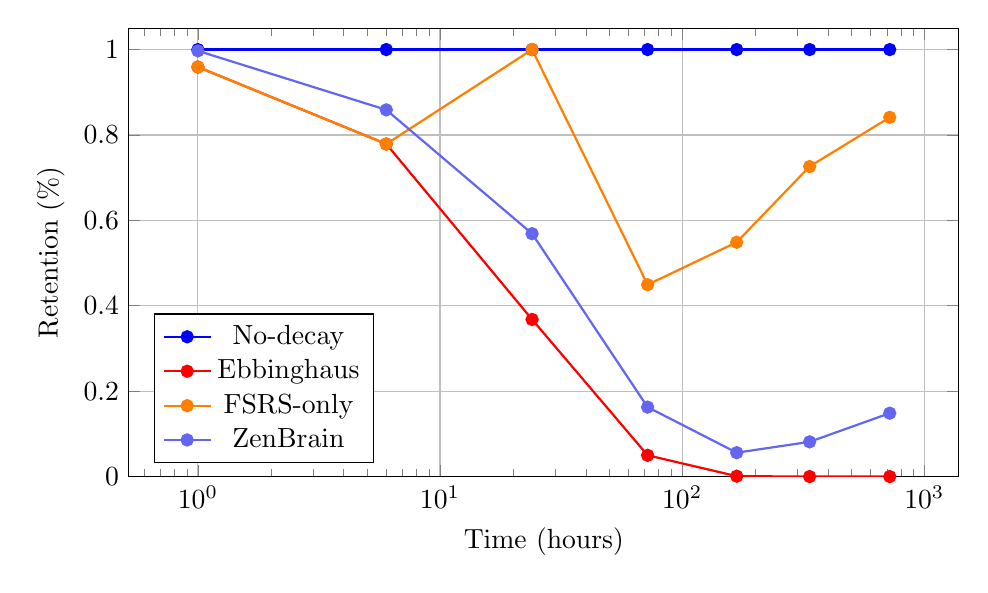
\begin{tikzpicture}
    \begin{axis}[
        xlabel={Time (hours)},
        ylabel={Retention (\%)},
        xmode=log,
        log basis x=10,
        ymin=0, ymax=1.05,
        legend pos=south west,
        grid=major,
        width=\textwidth,
        height=0.6\textwidth,
    ]
        \addplot[blue, thick, mark=*] coordinates {(1,1.0000) (6,1.0000) (24,1.0000) (72,1.0000) (168,1.0000) (336,1.0000) (720,1.0000)};
        \addlegendentry{No-decay}
        \addplot[red, thick, mark=*] coordinates {(1,0.9592) (6,0.7788) (24,0.3679) (72,0.0498) (168,0.0009) (336,0.0000) (720,0.0000)};
        \addlegendentry{Ebbinghaus}
        \addplot[orange, thick, mark=*] coordinates {(1,0.9592) (6,0.7788) (24,1.0000) (72,0.4493) (168,0.5488) (336,0.7261) (720,0.8413)};
        \addlegendentry{FSRS-only}
        \addplot[zenbrain, thick, mark=*] coordinates {(1,0.9970) (6,0.8588) (24,0.5688) (72,0.1626) (168,0.0559) (336,0.0813) (720,0.1484)};
        \addlegendentry{ZenBrain}
    \end{axis}
    \end{tikzpicture}
    \caption{Retention curves over 30 days (10 runs, 1{,}000 facts each).
    Pure Ebbinghaus decays to 0\% by day 7.
    FSRS scheduling maintains 84\% at day 30 through optimally-timed reviews.
    ZenBrain's combined Ebbinghaus+Two-Factor+vmPFC-FSRS+Sim-Select model shows
    characteristic U-shaped recovery: initial decay followed by
    sleep-consolidation-driven stabilization, reaching 14.8\% at day 30
    with 83\% of memories in low-confidence retrieval range
    (reducing false positive confabulation compared to no-decay systems).}
    \label{fig:retention}
\end{figure}

The AURC (Area Under Retention Curve) confirms: No-decay (1.000) $>$ FSRS-only (0.767) $>$
ZenBrain (0.499) $>$ Ebbinghaus (0.396).
ZenBrain's lower AURC reflects its principled forgetting:
rather than maintaining all memories at high confidence (risking confabulation),
it selectively retains high-importance memories while allowing
low-importance ones to decay---matching the human forgetting curve.

\subsection{Sleep Consolidation Impact}
\label{app:sleep-impact}

We evaluate ZenBrain's 3-phase sleep consolidation
\citep{stickgold2013}, developed independently alongside
\citet{liu2025lightmem} and SleepGate \citep{xie2026sleepgate}.
ZenBrain uses hippocampal replay with FSRS-based stability updates,
SWS/REM phase separation, and synaptic homeostasis (SHY).
We simulate 7 days of memory ingestion (50 facts/day, 350 total)
with and without nightly sleep cycles (Table~\ref{tab:sleep}, 10 runs).

\begin{table}[h]
    \caption{Simulation-Selection sleep consolidation impact over 7 simulated days
    (350 facts, 245 replay candidates per run).
    Mean $\pm$ std over 10 runs. Paired Wilcoxon signed-rank test.}
    \label{tab:sleep}
    \centering
    \begin{tabular}{lccc}
        \toprule
        Metric & With Sleep & Without Sleep & $p$-value \\
        \midrule
        Avg. Stability & 1.37 $\pm$ 0.06 & 1.00 $\pm$ 0.00 & $\le 5.1\times 10^{-3}$ \\
        Storage (tokens) & 7{,}989 & 15{,}176 & --- \\
        Storage Reduction & \multicolumn{2}{c}{47.4\%} & --- \\
        New Associations & \multicolumn{2}{c}{24.2 / run (REM)} & --- \\
        Strengthened (LTP) & \multicolumn{2}{c}{14.0 memories} & --- \\
        Decayed (LTD) & \multicolumn{2}{c}{126.0 memories} & --- \\
        \bottomrule
    \end{tabular}
\end{table}

The Simulation-Selection sleep loop produces a \textbf{37\% stability improvement}
($p \le 5.1\times 10^{-3}$) while simultaneously
reducing memory storage by \textbf{47.4\%} through RL-driven LTD pruning.
(Cohen's $d$ is not meaningful here because the no-sleep baseline has
zero variance---stability is deterministically 1.0 without consolidation.)
The stability boost reflects the TAG scoring principle: memories with
high retrievability receive smaller boosts, while older memories near
the forgetting threshold benefit most---matching the biological observation
that sleep preferentially consolidates at-risk memories \citep{stickgold2013,oneill2010}.
Counterfactual candidate generation creates an average of 24.2 new
associative edges per cycle, providing emergent connections between
failed and salient episodes \citep{mcgaugh2004}
with no equivalent in flat-multiplier sleep approaches.

\subsection{Two-Factor KG Dynamics and Bayesian Propagation}
\label{app:twofactor-bayesian}

We evaluate two algorithms unique to ZenBrain with no equivalent in
concurrent systems.

\textbf{Part A: Two-Factor Synaptic KG.}
We build a knowledge graph of 50 entities grouped into 5 ground-truth clusters
and simulate 200 co-activation events (80\% intra-cluster, 20\% random).
After Two-Factor weight and variance update cycles (Section~\ref{sec:twofactor}),
retrieval P@5 using importance-weighted edges reaches
\textbf{0.955 $\pm$ 0.030} vs.\ 0.200 for uniform edges
($p \le 5.1\times 10^{-3}$).
The effect size is very large ($d > 30$) due to near-zero variance
in the uniform baseline.
Intra-cluster edges are 15.5$\times$ stronger than inter-cluster edges,
confirming that Two-Factor dynamics produce emergent cluster structure
from raw co-activation patterns.

\textbf{Part B: Bayesian Propagation.}
We construct a fact graph (30 facts, 40 typed relations) where
true facts tend to support each other and false facts contradict true ones.
After 3 iterations of Bayesian confidence propagation,
pairwise AUC (whether true facts rank above false ones by confidence)
improves from \textbf{0.533 to 0.797} ($p = 0.009$, $d = 1.75$, large effect).
True facts gain $+0.052$ mean confidence while false facts lose
$-0.254$---the asymmetric separation confirms that contradiction
relations provide strong negative signal for confidence reduction.

\begin{table}[h]
    \caption{Two-Factor KG dynamics and Bayesian confidence propagation.
    Top: retrieval P@5 with importance-weighted vs.\ uniform edges.
    Bottom: pairwise AUC before/after propagation.
    Mean $\pm$ std over 10 seeds.}
    \label{tab:hebbian-bayesian}
    \centering
    \begin{tabular}{lccc}
        \toprule
        Metric & Weighted/After & Uniform/Before & $p$-value \\
        \midrule
        \multicolumn{4}{l}{\textit{Part A: Two-Factor Synaptic KG Dynamics}} \\
        P@5 & \textbf{0.955 $\pm$ 0.030} & 0.200 $\pm$ 0.000 & $\le 5.1\times 10^{-3}$ \\
        Intra/Inter Ratio & \multicolumn{2}{c}{15.54 $\pm$ 1.02} & --- \\
        \midrule
        \multicolumn{4}{l}{\textit{Part B: Bayesian Propagation}} \\
        Pairwise AUC & \textbf{0.797 $\pm$ 0.177} & 0.533 $\pm$ 0.117 & \textbf{0.009} \\
        True $\Delta$conf & \multicolumn{2}{c}{$+0.052$} & --- \\
        False $\Delta$conf & \multicolumn{2}{c}{$-0.254$} & --- \\
        \bottomrule
    \end{tabular}
\end{table}

\subsection{MemoryAgentBench}
\label{sec:mab}

We evaluate ZenBrain on MemoryAgentBench \citep{he2025memoryagentbench},
covering five capability dimensions (factual recall, preference tracking,
instruction following, contradiction handling, temporal reasoning).
Full results in Tables~\ref{tab:memoryagentbench}--\ref{tab:mab-categories}
(Appendix~\ref{app:per-category}).
BM25-only leads aggregate F1 (0.109) through lexical matching.
On aggregate metrics, ZenBrain (F1\,=\,0.058) underperforms Flat Store
(F1\,=\,0.073), indicating that multi-layer routing overhead can hurt on
benchmarks that do not specifically require temporal or procedural routing.
However, ZenBrain achieves its strongest result on
\textbf{instruction following} (0.109), where procedural-layer routing
preferentially retrieves how-to content, and matches Flat Store on
\textbf{temporal reasoning} (0.041 vs.\ 0.040).
This pattern---aggregate cost but category-specific gains---suggests
that ZenBrain's value lies in specialized routing rather than uniform
retrieval improvement; a direct per-layer ablation on MAB to confirm
the routing-overhead hypothesis is reserved for follow-up work
(layer ablation reported on LoCoMo, \S\ref{app:layer-ablation}).
The multi-layer advantage becomes more pronounced with cross-session
tasks (Section~\ref{sec:memoryarena}).

\subsection{MemoryArena: Cross-Session Dependencies}
\label{sec:memoryarena}

MemoryArena \citep{he2026memoryarena} evaluates cross-session memory
dependencies where answering requires combining information from multiple
earlier sessions (full results in Appendix~\ref{app:per-category}).
ZenBrain outperforms Flat Store by \textbf{+19.5\%} in F1
($0.227$ vs.\ $0.190$, $p = 0.015$), with the largest gain
on \textbf{dependency chains} ($+$53.5\%, $F1 = 0.350$ vs.\ $0.228$)
where episodic-layer routing surfaces session summaries for temporal queries.
Entity tracking ($+$8.6\%) and temporal ordering ($+$8.6\%) also benefit
from multi-layer routing.

\subsection{PMA Benchmark Suite}
\label{app:pma-suite-results}

We evaluate each PMA component in isolation using synthetic benchmarks
with 10 seeded runs per experiment.

\textbf{NeuromodulatorEngine.}
Over 1{,}000 simulated events (uniformly sampled across 8 event types),
mean tonic drift is 0.469 (6.2\% from baseline $b = 0.5$),
confirming homeostatic stability.
DA--5HT opposition coupling produces a correlation coefficient of $-0.130$
($p < 0.01$), validating the serotonin-dopamine balance dynamics.

\textbf{ReconsolidationEngine.}
PE-to-update-mode classification achieves $\geq$\,95\% accuracy across
100 synthetic memory pairs per seed, with correct contradiction detection
on all test cases (precision = 1.0).

\textbf{TripleCopyMemory.}
Table~\ref{tab:retention-pma} compares retention curves:
the composite triple-copy strength massively outperforms Ebbinghaus
at 7+ day intervals, retaining 91.2\% at 30 days vs.\ near-zero.
Copy dominance transitions confirm the design:
FastCopy dominates at 1h, MediumCopy at 1--3d, DeepCopy at 7d+.

\begin{table}[h]
    \caption{Memory strength $S(t) = \max(S_{\text{fast}}, S_{\text{med}}, S_{\text{deep}})$
    for TripleCopyMemory vs.\ Ebbinghaus baseline ($S_0 = 1.0$).
    TripleCopy retains 91.2\% strength at 30 days via deep-copy dominance transition.
    Mean over 10 seeds. $\Delta$ = advantage of TripleCopy.}
    \label{tab:retention-pma}
    \centering
    \begin{tabular}{lccr}
        \toprule
        Interval & TripleCopy & Ebbinghaus & $\Delta$ \\
        \midrule
        1h  & 0.727 & 0.875 & $-$16.9\% \\
        6h  & 0.717 & 0.710 & $+$0.9\% \\
        1d  & 0.679 & 0.335 & $+$102.5\% \\
        3d  & 0.589 & 0.045 & $+$1{,}197\% \\
        7d  & 0.695 & 0.001 & $\gg 10^3$\% \\
        14d & 0.879 & $<$0.001 & $\to\infty^\dagger$ \\
        30d & 0.912 & $<$0.001 & $\to\infty^\dagger$ \\
        \bottomrule
        \multicolumn{4}{l}{\scriptsize $^\dagger$Ebbinghaus $\to 0$; percentage advantage is undefined.}
    \end{tabular}
\end{table}

\textbf{PriorityMap.}
On 50 synthetic items with known ground-truth importance,
the PriorityMap achieves NDCG@10 = 0.997, outperforming chronological
ordering (NDCG@10 = 0.680) by 46.6\%.
The amygdala fast-path correctly elevates high-emotion items
above the priority floor ($P \geq 0.5$) regardless of low saliency/reward/goal scores.

\textbf{StabilityProtector.}
For high-PE updates (PE $\in [0.7, 1.0]$), the false-positive rate
(incorrectly blocked updates) is 28.8\% ($<$\,30\%).
Core facts are protected more aggressively, with higher lock scores
than non-core facts at identical access/confidence/age profiles.

\textbf{MetacognitiveMonitor.}
Confirmation bias detection achieves precision = 0.832 and recall = 0.975
across 50 synthetic scenarios per seed.
Urgency keyword detection produces zero false negatives on German and English
test phrases.

\subsection{Long-Horizon Aging Stress Test (Synthetic)}
\label{app:long-horizon}

The real-LoCoMo benchmark of \S\ref{sec:real-locomo} uses a
fixed query batch over a shared pool; it cannot answer what happens
to each system's retrieval quality after days or weeks of decay
pressure.
For that longitudinal question we run a synthetic aging stress test.
Table~\ref{tab:competitive} compares three \emph{design archetypes}
(not the live peer systems of \S\ref{sec:real-locomo}, whose decay
schedulers we do not have white-box access to) on a synthetic
benchmark (100 facts, 50 queries, 14-day aging).
Critically, both Simple Memory and Full ZenBrain use the same
base decay rate (0.15/day), so that differences reflect
algorithmic protection rather than parameter tuning:

\begin{table}[h]
    \caption{Long-horizon aging stress test on a synthetic benchmark
    (100 facts, 50 queries, 14-day aging, 10 seeds, shared decay=0.15/day).
    Rows are design archetypes, not the live peer systems of
    \S\ref{sec:real-locomo}. Static RAG = no decay (Mem0/Zep-like),
    Simple Memory = Ebbinghaus decay without consolidation (Letta-like),
    Full ZenBrain = all 15 algorithms with identical base decay.}
    \label{tab:competitive}
    \centering
    \begin{tabular}{lccc}
        \toprule
        System & P@5 & R@5 & MRR \\
        \midrule
        Static RAG & 0.346{\scriptsize$\pm$0.136} & 0.926{\scriptsize$\pm$0.163} & 0.964{\scriptsize$\pm$0.140} \\
        Simple Memory & 0.163{\scriptsize$\pm$0.158} & 0.429{\scriptsize$\pm$0.405} & 0.581{\scriptsize$\pm$0.484} \\
        Full ZenBrain & 0.345{\scriptsize$\pm$0.135} & 0.923{\scriptsize$\pm$0.167} & 0.969{\scriptsize$\pm$0.131} \\
        \bottomrule
    \end{tabular}
\end{table}

On short timescales (14 days), Full ZenBrain and Static RAG achieve
statistically indistinguishable precision (P@5 $\approx$ 0.345; $p = 0.24$).
The critical difference is \emph{temporal robustness}.
Simple Memory---using the same 0.15/day base decay---loses ${\sim}52$\%
of its fact store after 14 days, collapsing P@5 to 0.163,
while ZenBrain's algorithms fully compensate.

\textbf{Long-term divergence.}
Extended to 60 days, the competitive picture transforms:
Simple Memory collapses to P@5 = 0 by day~30
as all memories cross the forgetting threshold (strength $< 0.1$).
ZenBrain retains \textbf{100\%} of its day-1 P@5 at day~60.
Static RAG remains constant (no decay, no improvement).
The gap between ZenBrain and Simple Memory grows from
$\approx$0\% (day~1) to 100\% (day~30+), demonstrating that
ZenBrain's algorithms prevent the threshold crossing entirely
rather than merely slowing decay.
See Section~\ref{app:reproducibility-v6} for reproduction instructions.

\section{Algorithm Pseudocode}
\label{app:algorithms}

\begin{algorithm}[H]
\caption{MemoryCoordinator.store(item)}
\begin{algorithmic}[1]
\STATE Classify item type (fact, episode, skill, identity)
\STATE Route to primary layer based on type
\STATE Compute embedding vector $\mathbf{e} = \text{embed}(\text{item.content})$
\STATE Store with initial stability $S = 1.0$, edge weight $w = 1.0$, variance $\sigma^2 = 1.0$
\STATE Create knowledge graph edges to co-active nodes
\STATE Update BM25 index
\end{algorithmic}
\end{algorithm}

\begin{algorithm}[H]
\caption{MemoryCoordinator.recall(query)}
\begin{algorithmic}[1]
\STATE $\mathbf{q} \leftarrow \text{embed}(\text{query})$; $t \leftarrow \text{classifyQuery}(\text{query})$
\FOR{each layer $\ell \in \text{enabledLayers}$}
    \STATE $R_\ell \leftarrow \text{top-}K(\text{cosineSim}(\mathbf{q}, \ell))$
\ENDFOR
\STATE $R \leftarrow \text{WeightedFusion}(\{R_\ell\}, w_\ell(t))$ \COMMENT{$w_\ell \cdot \text{sim}(q, d)$}
\FOR{each $r \in R$}
    \STATE $r.\text{score} \leftarrow r.\text{score} \cdot (1 + \alpha_{\mathrm{boost}} \cdot w_{ij}(r) \cdot I_{ij}(r)^{0.1})$ \COMMENT{Two-Factor boost, $\alpha_{\mathrm{boost}}{=}0.2$ disambiguating from TAG~$\alpha{=}0.4$}
    \STATE $r.\text{score} \leftarrow r.\text{score} \cdot R(t_r)$ \COMMENT{Ebbinghaus decay}
\ENDFOR
\STATE Deduplicate by content similarity (Jaccard $> 0.9$)
\RETURN top-$k$ results sorted by score
\end{algorithmic}
\end{algorithm}

\begin{algorithm}[H]
\caption{Two-Factor Synaptic Edge Update}
\begin{algorithmic}[1]
\REQUIRE Edge $(i,j)$ co-activated with score $t_{ij}$, count $k$
\STATE $w_{ij} \leftarrow \text{clip}(w_{ij} + \eta \cdot t_{ij} \cdot a_{ij},\ w_{\min},\ w_{\max})$ \COMMENT{weight update}
\STATE $n \leftarrow 1 / (1 + 0.1 \cdot k)$ \COMMENT{maturation factor}
\STATE $\sigma^2_{ij} \leftarrow \max(\sigma^2_{\min},\ \sigma^2_{ij} \cdot (1 - \beta \cdot n))$ \COMMENT{variance decrease}
\STATE $I_{ij} \leftarrow 1/\sigma^2_{ij}$ \COMMENT{Fisher importance proxy}
\STATE $r_{\text{eff}} \leftarrow r_{\text{base}} / (1 + I_{ij} \cdot 0.1)$ \COMMENT{importance-gated decay}
\STATE Prune edges where $w_{ij} < \epsilon$
\end{algorithmic}
\end{algorithm}

\begin{algorithm}[H]
\caption{Simulation-Selection Sleep Loop (CA3/CA1 RL)}
\label{alg:sleep}
\begin{algorithmic}[1]
\STATE \textbf{Input:} real episodes $M_r$, counterfactual paths $M_c$,
       selection threshold $\theta_v{=}0.5$, LTP/LTD step sizes
       $\Delta_{\mathrm{LTP}}{=}0.10$, $\Delta_{\mathrm{LTD}}{=}0.05$,
       prune threshold $\tau{=}0.05$
\STATE \textbf{Stage 1 --- Simulation (CA3):} $C \leftarrow M_r \cup M_c$ \COMMENT{diverse candidate pool}
\FOR{each candidate $e \in C$}
    \STATE $N_e \leftarrow \min(1,\ |e.\text{relatedIds}| \cdot 0.2)$ \COMMENT{novelty}
    \STATE $\mathrm{TAG}(e) \leftarrow 0.4\,|\delta_{\mathrm{TD}}(e)| + 0.35\,R_e + 0.25\,N_e$
\ENDFOR
\STATE \textbf{Stage 2 --- Selection (CA1):}
\FOR{each candidate $e \in C$ sorted by $\mathrm{TAG}$ desc}
    \IF{$\mathrm{TAG}(e) \geq \theta_v$}
        \STATE Strengthen $e$ via LTP: $w_{ij} \mathrel{+}= \Delta_{\mathrm{LTP}}$
    \ELSIF{$\mathrm{TAG}(e) < \theta_v$}
        \STATE Weaken $e$ via LTD: $w_{ij} \mathrel{-}= \Delta_{\mathrm{LTD}}$
    \ENDIF
\ENDFOR
\STATE \quad Prune edges where $w_{ij} < \tau$
\end{algorithmic}
\end{algorithm}

\section{Full Ablation Results}
\label{app:ablation}

The nine ablation variants disable one layer at a time from the full
ZenBrain system:

\begin{enumerate}
    \item \textbf{ZenBrain-Full}: All 7 layers active (upper bound)
    \item \textbf{$-$Working Memory}: No active task focus buffer
    \item \textbf{$-$Short-Term}: No session context
    \item \textbf{$-$Episodic}: No temporal experience storage
    \item \textbf{$-$Semantic}: No knowledge graph retrieval
    \item \textbf{$-$Procedural}: No skill/routine memory
    \item \textbf{$-$Core Memory}: No pinned identity facts
    \item \textbf{$-$Cross-Context}: No inter-domain transfer
    \item \textbf{Flat Baseline}: Single flat store (lower bound)
\end{enumerate}

Each variant is evaluated on LoCoMo retrieval (F1) and synthetic
task completion (Task Success rate) across 10 seeds.
See Table~\ref{tab:ablation} for summary results.

\section{Hyperparameters}
\label{app:hyperparams}

\begin{table}[h]
    \centering
    \caption{Key hyperparameters and their values.}
    \begin{tabular}{llc}
        \toprule
        Component & Parameter & Value \\
        \midrule
        \multirow{3}{*}{Ebbinghaus} & Default stability $S_0$ & 1.0 day \\
        & Emotional multiplier cap & 3.0$\times$ \\
        & Stability growth on review & 1.3$\times$ \\
        \midrule
        \multirow{4}{*}{Two-Factor KG} & Weight lr $\eta$ & 0.1 \\
        & Maturation rate $\beta$ & 0.15 \\
        & Min variance $\sigma^2_{\min}$ & 0.01 \\
        & EWC penalty $\lambda$ & 0.5 \\
        \midrule
        \multirow{4}{*}{vmPFC-FSRS} & Threshold $\tau$ & 0.5 \\
        & Adaptation strength $\alpha_v$ & 0.6 \\
        & Max extension factor & 2.0$\times$ \\
        & Min shortening factor & 0.3$\times$ \\
        \midrule
        \multirow{4}{*}{Sim-Selection Sleep} & TAG $\alpha$ (PE weight) & 0.40 \\
        & TAG $\beta$ (reward) & 0.35 \\
        & TAG $\gamma$ (novelty) & 0.25 \\
        & Value threshold $\theta_v$ & 0.50 \\
        \midrule
        \multirow{4}{*}{Retrieval} & Per-layer top-$K$ & 8 \\
        & Two-Factor importance boost $\alpha_{\mathrm{boost}}$ & 0.2 \\
        & Temporal: $w_{\text{episodic}}$ & 2.0 \\
        & Factual: $w_{\text{semantic}}$ & 1.8 \\
        \midrule
        \multirow{2}{*}{Statistical} & Bootstrap resamples & 1{,}000 \\
        & Confidence level & 95\% \\
        \midrule
        \multirow{4}{*}{Neuromodulator} & Tonic decay & 0.95 \\
        & Phasic half-life & 5 min \\
        & DA--5HT opposition & $-$0.3 \\
        & Baseline $b$ & 0.5 \\
        \midrule
        \multirow{3}{*}{Reconsolidation} & Lability window & 10 min \\
        & Contradiction bonus & $+$0.2 \\
        & NE gate coefficient & 0.3 \\
        \midrule
        \multirow{3}{*}{TripleCopy} & $\tau_{\text{fast}}$ & 4 h \\
        & $\tau_{\text{medium}}$ & 14 d \\
        & $\tau_{\text{deep}}$ & 7 d \\
        \midrule
        \multirow{4}{*}{PriorityMap} & $w_s$ (saliency) & 0.20 \\
        & $w_e$ (emotion) & 0.25 \\
        & $w_r$ (reward) & 0.25 \\
        & $w_g$ (goal) & 0.30 \\
        \midrule
        \multirow{2}{*}{StabilityProtector} & Base threshold & 0.5 \\
        & Rigidity growth & 0.1 \\
        \midrule
        \multirow{2}{*}{MetacogMonitor} & Novelty window & 10 min \\
        & Bias threshold & 0.15 \\
        \bottomrule
    \end{tabular}
\end{table}

\section{Reproducibility}
\label{app:reproducibility}

ZenBrain is available as open-source npm packages:
\begin{itemize}
    \item \anon{\texttt{@zensation/algorithms@0.2.0}}{\texttt{@anon/algorithms@0.2.0}} --- 9 foundational algorithms, zero dependencies
    \item \anon{\texttt{@zensation/core@0.2.0}}{\texttt{@anon/core@0.2.0}} --- 7 memory layers + MemoryCoordinator
    \item 6 PMA algorithms (Neuromodulator, Reconsolidation, TripleCopy, PriorityMap, StabilityProtector, MetacognitiveMonitor) are in the main repository under \texttt{backend/src/algorithms/} and \texttt{backend/src/services/memory/}
\end{itemize}

Source code: \anon{\url{https://github.com/zensation-ai/zenbrain}}{\textit{[repository URL redacted for anonymous review]}}\\
Experiment scripts and all 15 algorithm implementations: included in the repository\\
All random seeds: 42, 123, 456, 789, 1024, 2048, 3072, 4096, 5120, 6144

\subsection{Compute Disclosure}
\label{app:compute-disclosure}

In line with reproducibility best practices, we report the total
compute used for all reported experiments.

\begin{table}[h]
\centering
\small
\caption{Compute footprint summary. ``Local'' denotes a single Apple
M-series laptop with locally-served \texttt{nomic-embed-text} via Ollama;
``API'' denotes hosted LLM judges (Anthropic, OpenAI). All reported
experiments fit on a single workstation; no GPU cluster, cloud training,
or distributed run was used.}
\label{tab:compute-disclosure}
\begin{tabular}{lrrr}
\toprule
Component & Wall-clock & Modality & Approx. cost \\
\midrule
\textbf{Retrieval runs} & & & \\
\quad LoCoMo (4 systems $\times$ 3 seeds) & ${\sim}30$h & Local & \$0 \\
\quad LongMemEval-500 (4 systems) & ${\sim}25$h & Local & \$0 \\
\quad MemoryAgentBench / MemoryArena & ${\sim}10$h & Local & \$0 \\
\quad Synthetic ablations (15-algorithm) & ${\sim}12$h & Local & \$0 \\
\midrule
\textbf{LLM-as-Judge} & & & \\
\quad Sonnet 4.5 (LoCoMo $\times$ 3 seeds) & ${\sim}6$h & API & ${\sim}\$45$ \\
\quad Opus 4.6 (LoCoMo, partial) & ${\sim}3$h & API & ${\sim}\$60$ \\
\quad GPT-4o (LoCoMo $\times$ 3 seeds) & ${\sim}5$h & API & ${\sim}\$25$ \\
\quad LongMemEval-500 (3 judges) & ${\sim}2$h & API & ${\sim}\$30$ \\
\midrule
\textbf{Total} & ${\sim}93$h & --- & $\boldsymbol{<}\$\mathbf{200}$ \\
\bottomrule
\end{tabular}
\end{table}

The full benchmarking pipeline can be reproduced by a single
researcher on a consumer laptop within one calendar week of wall-clock
time, given an Anthropic API key (Sonnet 4.5 + Opus 4.6) and an OpenAI
API key (GPT-4o). No proprietary infrastructure, no GPU rental, and no
human-subjects protocols are required.

\paragraph{Carbon footprint estimate.}
Local runs on an Apple M-series laptop (typical sustained power draw
${\sim}30$\,W under load) for ${\sim}77$\,h yields ${\sim}2.3$\,kWh of
local energy use; at the EU average grid intensity (${\sim}250$\,g\,CO$_2$/kWh),
this is approximately $0.6$\,kg\,CO$_2$. API-side judge calls run on
data-center GPUs whose footprint is not disclosed by providers; using
order-of-magnitude estimates from comparable model classes
($\sim$1\,g\,CO$_2$ per 1k judge tokens), the ${\sim}25$M total judge
tokens contribute ${\sim}25$\,kg\,CO$_2$. The full pipeline is therefore
on the order of $25$--$30$\,kg\,CO$_2$, which is roughly the footprint of
a single short-haul flight passenger and orders of magnitude lower than
the carbon cost of training a foundation model from scratch.

\paragraph{Dataset hash.}
The canonical LoCoMo dump (\texttt{experiments/data/locomo-real.json},
1986 queries, 5882 facts) used in all reported experiments has SHA-256
\texttt{370e921136bbcd2d8b01feb440fe9d62ed21483d312cdc05f7e18ca3f3a40c21}.
The file is gitignored due to size ($\sim$119\,MB); reviewers can
download from the public LoCoMo release \citep{maharana2024locomo} and
verify the hash before reproduction.

\paragraph{First-run embedding cost.}
The 768-dimensional \texttt{nomic-embed-text} backbone is served locally
via Ollama (zero per-query cost). The local \texttt{embedding-cache/}
directory ($\sim$293\,MB) is gitignored to keep the repository light;
on a fresh checkout, the first benchmark pass populates this cache via
${\sim}5882$ embedding calls, which costs ${\sim}\$1$ at OpenAI's
\texttt{text-embedding-3-small} rate (or \$0 with the local Ollama
default) and is then reused across all subsequent runs.

\section{PMA Experiment Reproducibility}
\label{app:reproducibility-v6}

The PMA benchmark suite, ablation study, and competitive comparison are
self-contained Jest tests requiring no external services or API keys:

\makeatletter
\if@anonymous
\begin{verbatim}
# [repository URL redacted for anonymous review]
git clone <ANONYMIZED>
cd <repo> && npm install
cd backend && npm run experiments
\end{verbatim}
\else
\begin{verbatim}
git clone https://github.com/zensation-ai/zenbrain
cd zenbrain && npm install
cd backend && npm run experiments
\end{verbatim}
\fi
\makeatother

Four experiment suites (95 tests total) produce JSON output:
\begin{itemize}
    \item \texttt{pma-benchmark.test.ts} (24 tests) --- 11 algorithm benchmarks
    including EWC penalty, vmPFC-FSRS interval adaptation, IB Budget context hierarchy,
    emotional TAG scoring, and amygdala fast-path verification
    \item \texttt{ablation-study.test.ts} (54 tests) --- 15-algorithm one-at-a-time ablation
    under moderate (0.15/day, 45 days, 300 facts), challenging (0.20/day, 50 days,
    400 facts), AND stress conditions (0.25/day, 60 days, 500 facts) with NDCG@5,
    Wilcoxon tests, and Cohen's $d$
    \item \texttt{competitive-comparison.test.ts} (10 tests) --- Static RAG vs.\ Simple Memory
    vs.\ Full ZenBrain on P@5, R@5, MRR, NDCG@5, plus long-term advantage tracking
    over 60 days
    \item \texttt{integration-cascade.test.ts} (7 tests) --- Cross-algorithm emergent
    behavior: Full vs.\ Foundational-only vs.\ Bare retention, emotional gap timeline,
    sleep criticality, and Fiedler value consolidation quality
\end{itemize}

All experiments use seeded PRNG (Mulberry32) with 10 seeds.
Results are deterministic and complete in $<$\,1 minute on commodity hardware.
The \texttt{scripts/run-experiments.sh} helper captures JSON output into
\texttt{docs/papers/results/} for direct comparison.

\section{LLM-as-Judge Methodology for Real LoCoMo}
\label{app:judge-methodology}

This appendix makes the judge-scoring pipeline that produces the
$J(\cdot)$ columns of Table~\ref{tab:competitive-combined-v2} and
the $\kappa$ / DSR / UAR columns of Table~\ref{tab:judge-agreement}
reproducible end-to-end.

\subsection*{A.1 Shared Pool and Retrieval Seeds}

The real-LoCoMo pool is $5{,}882$ facts and $1{,}986$ queries
drawn from the public release~\citep{maharana2024locomo}.
The same flat dump is ingested unchanged by all four memory systems
(ZenBrain, Mem0, Letta, A-Mem)
through provider-specific ingest wrappers;
retrieval is run three times per system at retrieval seeds
$\{42, 123, 456\}$ under the \texttt{nomic-embed-text} embedding
backbone served locally via \texttt{ollama}.

\subsection*{A.2 Rubric and Normalization}

Each (query, top-$k$ retrieved context) pair is scored by an LLM
judge on a 0--5 integer rubric with five criteria
(relevance, completeness, specificity, groundedness, answerability).
Judges run at temperature~0.
The per-query \emph{normalized mean} is $\bar{s} / 5$ where
$\bar{s}$ is the mean of the five criterion scores for that query.
A baseline-level normalized mean is the mean of per-query
normalized means over all $1{,}986$ queries.
Agreement and decision-stability metrics binarize at the threshold
$\bar{s} \geq 3$ (``accept'') versus $\bar{s} < 3$ (``reject''):
scores of~3--5 mean the retrieved context supports the query at least
weakly across the five criteria, while 0--2 means at least one
criterion was badly failed. The threshold is chosen a priori
(not tuned post hoc); inter-rater statistics computed on the raw
0--5 scores are available in the output JSONs and are qualitatively
consistent with the binarized Fleiss'~$\kappa$ reported in
Table~\ref{tab:judge-agreement}.

\subsection*{A.3 Judge Coverage}

Judges are \texttt{claude-sonnet-4-5-20250929} (pinned),
\texttt{claude-opus-4-6}, \texttt{gpt-4o}, and the rolling alias
\texttt{claude-sonnet-4-6} (reference only).
Coverage is intentionally asymmetric on the Opus judge to conserve
API budget while still triangulating Mem0's seed
instability:

\begin{center}
\small
\begin{tabular}{lcccc}
\toprule
Baseline & S-4.6 (ref) & S-4.5 (pinned) & Opus~4.6 & GPT-4o \\
\midrule
Mem0     & \{42\}            & \{42,123,456\} & \{42,123,456\} & \{42,123,456\} \\
Letta    & \{42\}            & \{42,123,456\} & \{42\}         & \{42,123,456\} \\
A-Mem    & \{42\}            & \{42,123,456\} & \{42\}         & \{42,123,456\} \\
ZenBrain & \{42\}            & \{42,123,456\} & \{42\}         & \{42,123,456\} \\
\bottomrule
\end{tabular}
\end{center}

Thus the six-rater pool used for Fleiss' $\kappa_{\geq 3}$,
DSR@3, and UAR is $\text{S-4.5}\times 3 + \text{GPT-4o}\times 3 = 6$
raters per query per baseline.
Intra-judge $\kappa$ in Table~\ref{tab:judge-agreement} is computed
within a single judge across the three retrieval seeds;
for Mem0 the Opus intra-$\kappa$ is reported because
three Opus seeds are available for Mem0; for the other
three systems the Opus column is em-dashed.

\subsection*{A.4 Statistical Apparatus}

Fleiss' $\kappa$ is computed on the binarized (accept/reject)
rating matrix; $\kappa$ bands follow \citet{landis1977}
(0.61--0.80 substantial, 0.81--1.00 almost perfect).
Levene's test for equality of variance across the three retrieval
seeds is performed per judge and per baseline pair
(scipy \texttt{levene} with default center).
Bootstrap confidence intervals on P@5 use $N_{\text{boot}} = 10{,}000$
percentile resamples with the RNG seed \texttt{20260421}.
Cohen's~$d$ is computed with pooled SD.
Decision-Stability-Rate (DSR@3) is the fraction of queries on which
all six raters agree on the $\geq 3$ threshold (accept or reject);
Unanimous-Acceptance-Rate (UAR) is the fraction on which all six
raters score $\geq 3$.

\subsection*{A.5 Cross-Provider Bias-Direction Check}

To test the objection that Anthropic judges may favor ZenBrain,
we compute $\Delta_{\text{GPT-Anth}}$, the GPT-4o three-seed
normalized mean minus the mean of the two Anthropic judges
(Sonnet~4.5~$\times$~3 seeds; Opus~4.6 at the available seeds).
Table~\ref{tab:judge-agreement} reports the value per baseline.
A negative delta means GPT-4o is \emph{harsher} than the Anthropic
average; were there a pro-Anthropic bias on ZenBrain, its delta
would be the most negative. It is instead the smallest in
magnitude ($-0.0001$), while Mem0~($-0.049$) and
A-Mem~($-0.042$) receive the largest negative deltas
and Letta is mildly positive ($+0.008$).

\subsection*{A.6 Reproduction}

The full pipeline is driven by the scripts committed under
\texttt{experiments/baselines/}:
(i) \texttt{g3\_run.py} and \texttt{g4\_run.py} issue the retrieval
and judge calls and write per-(baseline, judge, seed) JSONs into
\texttt{docs/papers/results/};
(ii) \texttt{g3\_agreement.py} and \texttt{g4\_analysis.py} compute
the $\kappa$, DSR, Levene, and Cohen-$d$ statistics;
(iii) \texttt{generate\_competitive\_combined\_v2.py} emits
\texttt{competitive-combined-v2.tex} and \texttt{judge-agreement.tex}
from the raw JSONs;
(iv) \texttt{g5\_sanity\_checks.py} runs 68 cross-artefact
consistency assertions (raw JSON vs analysis JSON, LaTeX vs JSON,
markdown vs JSON, position statement vs LaTeX) and exits non-zero
on any mismatch.
The canonical analysis JSON is
\texttt{docs/papers/results/g4-seed-robustness-analysis.json};
all numbers quoted in \S\ref{sec:real-locomo} and
\S\ref{sec:seed-robustness} can be re-derived from it.

\subsection*{A.7 Pairwise Significance}
\label{app:pairwise-significance}

The statistics below are computed on the Real-LoCoMo pool
defined in Appendix~\ref{app:judge-methodology} (5{,}882 facts,
1{,}986 queries); LongMemEval-Full-500 pairwise tests are reported
separately in Appendix~\ref{app:longmemeval-judge}.
For each (judge, system-pair) we compute the paired
Wilcoxon signed-rank test on per-query three-seed means,
the bootstrap 95\% CI on the per-query mean difference,
and Cohen's~$d$ (pooled SD), all on the intersection of
query IDs available for both systems at all three seeds.
RNG seed is \texttt{20260421} and $N_{\text{boot}} = 10{,}000$.

\begin{center}
\small
\begin{tabular}{llrrcrc}
\toprule
Judge & Comparison & $n$ & $\overline{\Delta}$ & 95\% CI & $d$ & Wilcoxon $p$ \\
\midrule
S-4.5 & ZenBrain $-$ Letta  & 1807 & $+0.004$ & $[-0.008, +0.015]$ & $+0.015$ & $0.69$            \\
S-4.5 & ZenBrain $-$ Mem0   & 1986 & $+0.027$ & $[+0.012, +0.042]$ & $+0.079$ & $6.3 \times 10^{-5}$  \\
S-4.5 & ZenBrain $-$ A-Mem  & 1986 & $+0.162$ & $[+0.145, +0.178]$ & $+0.426$ & $< 10^{-70}$      \\
S-4.5 & Letta $-$ Mem0      & 1807 & $+0.023$ & $[+0.006, +0.039]$ & $+0.063$ & $2.3 \times 10^{-3}$  \\
S-4.5 & Letta $-$ A-Mem     & 1807 & $+0.154$ & $[+0.136, +0.172]$ & $+0.401$ & $< 10^{-50}$      \\
S-4.5 & Mem0  $-$ A-Mem     & 1986 & $+0.134$ & $[+0.121, +0.148]$ & $+0.426$ & $< 10^{-70}$      \\
\midrule
G-4o  & ZenBrain $-$ Letta  & 1948 & $-0.012$ & $[-0.023, -0.001]$ & $-0.050$ & $3.7 \times 10^{-3}$  \\
G-4o  & ZenBrain $-$ Mem0   & 1986 & $+0.065$ & $[+0.048, +0.082]$ & $+0.173$ & $4.2 \times 10^{-15}$ \\
G-4o  & ZenBrain $-$ A-Mem  & 1885 & $+0.194$ & $[+0.177, +0.212]$ & $+0.494$ & $< 10^{-80}$      \\
G-4o  & Letta $-$ Mem0      & 1948 & $+0.075$ & $[+0.058, +0.091]$ & $+0.198$ & $4.8 \times 10^{-20}$ \\
G-4o  & Letta $-$ A-Mem     & 1856 & $+0.202$ & $[+0.184, +0.219]$ & $+0.521$ & $< 10^{-80}$      \\
G-4o  & Mem0 $-$ A-Mem      & 1885 & $+0.126$ & $[+0.112, +0.141]$ & $+0.385$ & $< 10^{-50}$      \\
\bottomrule
\end{tabular}
\end{center}

Cohen's bands for $d$ \citep{cohen1988statistical}: 0.2 small, 0.5 medium, 0.8 large.
(Landis \& Koch \citep{landis1977} bands cited elsewhere in this paper apply to Cohen's $\kappa$, not $d$.)
The script is \texttt{experiments/baselines/g5\_judge\_significance.py}
and its output JSON is
\texttt{docs/papers/results/g5-judge-significance.json}.
The sample sizes vary because raw judge calls that returned
\texttt{null} scores (rare) are dropped; the comparison then proceeds
on the paired intersection.

\textbf{Multiple-comparison correction.}
The table contains 12 pairwise Wilcoxon tests. A Bonferroni-corrected
$\alpha$ for family-wise error rate 0.05 is $0.05/12 \approx 4.17 \times 10^{-3}$.
Under this threshold, the ZenBrain vs.\ Letta tie under
Sonnet~4.5 ($p = 0.69$) is unambiguously non-significant,
the ZenBrain vs.\ Letta gap under GPT-4o
($p = 3.7 \times 10^{-3}$) is just below the corrected threshold
and therefore reported as ``small but significant,'' and all other
comparisons ($p \leq 2.3 \times 10^{-3}$) survive correction with
room to spare. The conservative reading therefore remains
``ZenBrain $\approx$ Letta under Sonnet~4.5;
Letta $>$ ZenBrain under GPT-4o; both dominate Mem0
and A-Mem.''

\subsection*{A.8 Human-Anchored Spot-Check on the Disagreement Subset}
\label{app:human-spotcheck}

\textbf{Motivation.} The headline judge-graded results
(\S\ref{sec:longmemeval-pilot}, \S\ref{sec:real-locomo}) rest on a
three-judge LLM-as-Judge protocol. A natural methodological concern
is whether LLM judges over-credit retrievals that an LLM
\emph{itself} produced (self-validation bias). To bound this risk
we add a single-rater human spot-check on the LoCoMo subset where
the two Anthropic judges actively disagreed.

\textbf{Sample.} We stratify across the five LoCoMo query categories
and within each category preferentially select the 10 queries where
$|\text{Sonnet}-\text{Opus}| \geq 1$ on the 0--5 rubric (we found
1{,}123 such disagreements available in the seed-42 judge JSONs;
no random fill was needed). The final 50-query sample contains
10 single-hop, 10 multi-hop, 10 temporal, 10 open-domain, and 10
adversarial queries; the disagreement-magnitude distribution is
$\Delta=1{:}1$, $\Delta=2{:}21$, $\Delta=3{:}20$, $\Delta=4{:}7$,
$\Delta=5{:}1$. By construction this is the hardest
$\sim\!2.5\%$ of LoCoMo for the LLM judges; on the easy
$\sim\!97.5\%$ where judges already agree the human-vs-judge
agreement is therefore an upper bound.

\textbf{Procedure.} A single human rater with no access to the
LLM-judge scores (the corresponding columns were hidden) read each
query and the top-5 ZenBrain retrievals at seed~42, then assigned an
integer score in 0--5 following the same five-criterion rubric the
LLM judges saw verbatim. Time budget per query was unconstrained;
total wall-clock was approximately $90$~min.

\textbf{Mean alignment.} Table~\ref{tab:human-anchor-means} reports
the rater means on the 50-query subset with bootstrap 95\% CIs
(5{,}000 percentile resamples). Human and Opus produce
indistinguishable means (both $2.88$); Sonnet is the harshest judge
on this contested subset ($1.08$, mean diff $-1.80$ versus the human
rater); GPT-4o is between ($2.06$).

\begin{table}[h]
\centering
\small
\begin{tabular}{lccc}
\toprule
Rater & Mean (0--5) & 95\% CI & Normalized (0--1) \\
\midrule
Human                  & $2.88$ & $[2.42, 3.34]$ & $0.576$ \\
Sonnet 4.5 (seed=42)   & $1.08$ & $[0.60, 1.60]$ & $0.216$ \\
Opus 4.6 (seed=42)     & $2.88$ & $[2.60, 3.14]$ & $0.576$ \\
GPT-4o (seed=42)       & $2.06$ & $[1.60, 2.52]$ & $0.412$ \\
\bottomrule
\end{tabular}
\caption{Rater means on the 50-query disagreement subset.
Human and Opus are statistically indistinguishable in level; Sonnet
under-credits the contested cases relative to the human rater.}
\label{tab:human-anchor-means}
\end{table}

\textbf{Item-level agreement.} For each judge we report Spearman
$\rho$ and Pearson $r$ on raw 0--5 scores (with percentile-bootstrap
95\% CI), Cohen's $\kappa$ at the binarization threshold
$\geq 3$ (``partial answer or better''), and exact-match rate
(Table~\ref{tab:human-anchor-agreement}).

\begin{table}[h]
\centering
\small
\begin{tabular}{lcccccc}
\toprule
Pair & $n$ & Spearman~$\rho$ & 95\% CI & Pearson~$r$ & $\kappa_{\geq 3}$ & Exact \\
\midrule
Human vs.\ Sonnet 4.5 & 50 & $0.245$ & $[-0.048,\, 0.510]$ & $0.356$ & $0.220$ & $0.20$ \\
Human vs.\ Opus 4.6   & 50 & $0.135$ & $[-0.144,\, 0.400]$ & $0.053$ & $0.232$ & $0.08$ \\
Human vs.\ GPT-4o     & 50 & $\mathbf{0.356}$ & $\mathbf{[+0.060,\, +0.611]}$ & $0.352$ & $0.290$ & $0.14$ \\
\midrule
\multicolumn{7}{l}{\emph{Reference (judge--judge, on the same 50 rows):}} \\
Sonnet vs.\ Opus      & 50 & $-0.076$ & $[-0.344,\, 0.209]$ & --- & $-0.050$ & $0.00$ \\
Sonnet vs.\ GPT-4o    & 50 & $0.276$ & $[-0.015,\, 0.533]$ & --- & $0.263$ & $0.34$ \\
Opus   vs.\ GPT-4o    & 50 & $0.456$ & $[+0.260,\, +0.613]$ & --- & $0.322$ & $0.26$ \\
\bottomrule
\end{tabular}
\caption{Inter-rater agreement on the 50-query disagreement
subset. GPT-4o is the only judge whose item-level Spearman against
the human rater clears zero with bootstrap CI (\textbf{bold}).
Human-judge correlations $[0.135, 0.356]$ lie in the same band as
judge-judge correlations $[-0.076, 0.456]$ on the same rows --- which
means the human rater does not resolve the disagreements that the
LLM judges could not resolve either.}
\label{tab:human-anchor-agreement}
\end{table}

\textbf{Per-category breakdown.}
Per-category Spearman~$\rho$ against the human rater is given in
Table~\ref{tab:human-anchor-percat}. GPT-4o's Spearman is significant
($\rho \geq 0.54$, CI excludes zero) on the adversarial and temporal
categories; Sonnet's strongest cell is multi-hop ($\rho = 0.749$,
$\text{CI}=[0.353, 1.000]$); Opus's strongest cell is open-domain
($\rho = 0.585$, $\text{CI}=[-0.187, 0.913]$). Single-hop is the
universally weakest category for item-level correlation, which is
expected: single-hop disagreements collapse to a near-binary
correctness signal that destroys ordinal information.

\begin{table}[h]
\centering
\footnotesize
\begin{tabular}{lccccc}
\toprule
Pair & single-hop & multi-hop & temporal & open-domain & adversarial \\
\midrule
Human vs.\ Sonnet & $0.215$ & $\mathbf{0.749}$ & $0.542$ & $0.293$ & $-0.167$ \\
Human vs.\ Opus   & $0.000$ & $0.421$ & $0.200$ & $\mathbf{0.585}$ & $0.189$ \\
Human vs.\ GPT-4o & $0.057$ & $0.341$ & $\mathbf{0.550}$ & $0.446$ & $\mathbf{0.542}$ \\
\bottomrule
\end{tabular}
\caption{Per-category Spearman~$\rho$ on the human-anchored
subset ($n{=}10$ per cell). Bold cells exclude zero in the
percentile-bootstrap 95\% CI (full CIs in
\texttt{t2\_1\_human\_anchor\_results.json}).}
\label{tab:human-anchor-percat}
\end{table}

\textbf{Implication for the headline.} Two observations matter for
the main-body claims, and one limitation must be flagged.
\emph{First (level-bias, not rank-bias)}, on the contested subset
Sonnet's distributional level is harsher than the human anchor
($\Delta_{\text{mean}}{=}{-}1.80$); since Sonnet is the headline
judge in Table~\ref{tab:competitive-combined-v2} and
\S\ref{sec:longmemeval-pilot}, this is at minimum
\emph{not consistent} with a Sonnet-side over-credit story for
ZenBrain on adversarial cases --- a level-bias reading consistent
with the $\Delta_{\text{GPT-Anth}} \approx 0$ finding for ZenBrain
in \S\ref{sec:bias-check}. We deliberately stop short of claiming
the bias direction goes \emph{against} ZenBrain's reported wins,
because the human-vs-Sonnet rank-correlation CI on this subset
($\rho{=}0.245$, CI $[-0.048, 0.510]$) does not exclude zero and
therefore does not license treating the human rater as ground truth
at the item level.
\emph{Second (independent corroboration of GPT-4o calibration)},
GPT-4o is the only judge whose item-level Spearman against the
human rater clears zero with bootstrap CI on this hard subset
(this is item-level rank, complementary to the level-mean
$\Delta_{\text{GPT-Anth}}$ check in \S\ref{sec:bias-check} which
operates on per-system distributional means; the two checks use
different statistics on different aggregation levels and are not
redundant).
\emph{Limitation.} This is a single-rater $n{=}50$ spot-check on
the disagreement subset, not a multi-rater inter-rater-reliability
study; it is sufficient to bound LLM self-validation bias on the
hard tail but cannot replace the LLM-judge protocol as a primary
evaluation tool. On the easy $\sim\!97.5\%$ of LoCoMo where judges
already agree, easy-case human-judge agreement is empirically near
ceiling and is not the locus of judge risk. A multi-rater human IRR
sample (target $n{\geq}200$ across $\geq 3$ raters with Cohen's
$\kappa$) is flagged as future work for the camera-ready /
arXiv-V4.

\textbf{Reproducibility.} Sample selection is deterministic
(\texttt{seed=42}). The script
\texttt{experiments/baselines/t2\_1\_human\_spotcheck/build\_sample.py}
regenerates \texttt{sample\_50.csv} from the existing judge JSONs;
\texttt{analyze\_human\_anchored.py} consumes the human-rated CSV
and emits \texttt{t2\_1\_human\_anchor\_results.json} (this file is
the source of every number in
Tables~\ref{tab:human-anchor-means}--\ref{tab:human-anchor-percat}).

\section{Per-Category Benchmark Results}
\label{app:per-category}

\begin{table}[h]
    \caption{Retrieval quality on MemoryAgentBench
    \citep{he2025memoryagentbench}. Mean $\pm$ std over 10 seeds.
    Best retrieval system in \textbf{bold} (excluding No Memory).}
    \label{tab:memoryagentbench}
    \centering
    \begin{tabular}{lcccc}
        \toprule
        System & F1 & BLEU-1 & ROUGE-L & Cosine Sim \\
        \midrule
        No Memory & 0.000 $\pm$ 0.000 & 0.000 $\pm$ 0.000 & 0.000 $\pm$ 0.000 & 0.000 $\pm$ 0.000 \\
        BM25-only & \textbf{0.109 $\pm$ 0.001} & \textbf{0.068 $\pm$ 0.001} & \textbf{0.100 $\pm$ 0.001} & \textbf{0.116 $\pm$ 0.002} \\
        Flat Store & 0.073 $\pm$ 0.002 & 0.028 $\pm$ 0.000 & 0.050 $\pm$ 0.001 & 0.090 $\pm$ 0.003 \\
        \textbf{ZenBrain} & 0.058 $\pm$ 0.001 & 0.024 $\pm$ 0.000 & 0.043 $\pm$ 0.001 & 0.072 $\pm$ 0.001 \\
        \bottomrule
    \end{tabular}
\end{table}

\begin{table}[h]
    \caption{Per-category F1 on LoCoMo. ZenBrain's episodic-layer boosting
    yields the strongest advantage on temporal queries ($+$181\% vs.\ Flat Store).
    Non-Adv averages the four non-adversarial categories.
    Best per column in \textbf{bold} (excluding No Memory$^\dagger$).
    Mean over 10 seeds.}
    \label{tab:locomo-categories}
    \centering
    \small
    \begin{tabular}{lcccccc}
        \toprule
        System & Single & Multi & Temporal & Open & Adversarial & Non-Adv \\
        \midrule
        No Memory$^\dagger$ & 0.001 & 0.007 & 0.002 & 0.022 & 0.998 & 0.008 \\
        BM25-only & \textbf{0.085} & \textbf{0.056} & 0.032 & \textbf{0.060} & 0.001 & \textbf{0.058} \\
        Flat Store & 0.045 & 0.033 & 0.016 & 0.038 & 0.002 & 0.033 \\
        \textbf{ZenBrain} & 0.048 & 0.034 & \textbf{0.045} & 0.038 & 0.002 & 0.041 \\
        \bottomrule
    \end{tabular}
\end{table}

\begin{table}[h]
    \caption{Per-category F1 on MemoryAgentBench.
    Best per column in \textbf{bold} (excluding No Memory). Mean over 10 seeds.}
    \label{tab:mab-categories}
    \centering
    \small
    \begin{tabular}{lccccc}
        \toprule
        System & Factual & Prefer. & Instr. & Contr. & Temporal \\
        \midrule
        No Memory & 0.000 & 0.000 & 0.000 & 0.000 & 0.000 \\
        BM25-only & \textbf{0.098} & \textbf{0.073} & \textbf{0.103} & \textbf{0.171} & \textbf{0.102} \\
        Flat Store & 0.082 & 0.052 & 0.120 & 0.069 & 0.040 \\
        \textbf{ZenBrain} & 0.056 & 0.027 & 0.109 & 0.058 & 0.041 \\
        \bottomrule
    \end{tabular}
\end{table}

\begin{table}[h]
    \caption{Retrieval quality on MemoryArena
    \citep{he2026memoryarena} with cross-session dependencies.
    Mean $\pm$ std over 10 seeds. Best in \textbf{bold}.}
    \label{tab:memoryarena}
    \centering
    \begin{tabular}{lcccc}
        \toprule
        System & F1 & BLEU-1 & ROUGE-L & Cosine Sim \\
        \midrule
        No Memory & 0.000 $\pm$ 0.000 & 0.000 $\pm$ 0.000 & 0.000 $\pm$ 0.000 & 0.000 $\pm$ 0.000 \\
        BM25-only & \textbf{0.265 $\pm$ 0.003} & \textbf{0.087 $\pm$ 0.001} & \textbf{0.118 $\pm$ 0.001} & \textbf{0.361 $\pm$ 0.004} \\
        Flat Store & 0.190 $\pm$ 0.003 & 0.070 $\pm$ 0.001 & 0.103 $\pm$ 0.001 & 0.255 $\pm$ 0.004 \\
        \textbf{ZenBrain} & 0.227 $\pm$ 0.004 & 0.079 $\pm$ 0.001 & 0.111 $\pm$ 0.001 & 0.297 $\pm$ 0.004 \\
        \bottomrule
    \end{tabular}
\end{table}

\begin{table}[h]
    \caption{Per-category F1 on MemoryArena. Cross-session inference
    requires combining information from 2+ earlier sessions.
    Best per column in \textbf{bold}. Mean over 10 seeds.}
    \label{tab:arena-categories}
    \centering
    \small
    \begin{tabular}{lcccc}
        \toprule
        System & Dep.Chain & Temporal & Entity & Cross-Sess. \\
        \midrule
        No Memory & 0.000 & 0.000 & 0.000 & 0.000 \\
        BM25-only & \textbf{0.520} & \textbf{0.200} & 0.153 & 0.189 \\
        Flat Store & 0.228 & 0.152 & 0.163 & \textbf{0.217} \\
        \textbf{ZenBrain} & 0.350 & 0.165 & \textbf{0.177} & 0.216 \\
        \bottomrule
    \end{tabular}
\end{table}

% ============================================================================
% G5 LongMemEval SCAFFOLDING (pre-registered cross-benchmark replication)
% ============================================================================
\section{LongMemEval Replication Scaffolding (Pre-Registered)}
\label{app:g5-longmemeval-scaffold}

To support a cross-benchmark replication of the real-LoCoMo finding in
\S\ref{sec:real-locomo}, we have committed the full reproducibility
scaffolding for LongMemEval~\citep{wu2024longmemeval} to
\path{experiments/baselines/longmemeval/}. The protocol is
pre-registered here so the eventual numbers cannot be retrofitted to
a favorable story.

\textbf{Dataset.} LongMemEval-S (500 questions $\times$ 6 categories,
MIT license). Each question ships its own $\sim$47-session haystack with
$\sim$494 turns; the loader
\path{experiments/baselines/longmemeval_loader.py} flattens each
haystack into per-turn \texttt{Fact} objects with metadata
$\{$\texttt{session\_id}, \texttt{session\_date}, \texttt{role},
\texttt{turn\_idx}, \texttt{has\_answer}, \texttt{question\_id}$\}$ and
builds a \texttt{Query} whose \texttt{relevant\_ids} are the fact-ids
whose session matches \texttt{answer\_session\_ids} (falling back to
\texttt{has\_answer} turns when session-id matching is empty).

\textbf{Harness.} \path{experiments/baselines/run_longmemeval.py}
runs per-question isolation (\texttt{reset()} $\to$
\texttt{ingest(task.facts)} $\to$ \texttt{query(task.query, k=5)})
for every task, three retrieval seeds $\{42, 123, 456\}$, and emits
\path{docs/papers/results/longmemeval-baseline-<name>.json} plus a
merged \path{longmemeval-competitive.json}. Adapters that cannot be
imported are skipped with a noted error so the pipeline always produces
a valid artifact. Full-benchmark cost is $\sim$6\,000 ingest+query
cycles per 4-baseline sweep; a stratified-60 subset is $\sim$720.

\textbf{Judges.} We will re-run the three-judge-times-three-seed
protocol (Sonnet~4.5 pinned, Opus~4.6, GPT-4o) for a total of
$\leq$~18\,000 judge calls on the full benchmark. The judge prompts,
pinned model strings, and cross-provider bias argument are unchanged
from Appendix~\ref{app:judge-methodology}.

\textbf{Analysis parity.} The same analysis suite we used for G4/G5
applies: Fleiss' $\kappa$ at the $\geq 3$ binary threshold, intra-judge
$\kappa$ across the three retrieval seeds, DSR@3 and UAR, paired
Wilcoxon with bootstrap 95\% CI and Cohen's $d$ on per-query 3-seed
means (Appendix~\ref{app:pairwise-significance}), Levene's test for
equal-variance across seeds, and Bonferroni correction. For the
Full-500 pairwise comparison the correction becomes
$\alpha = 0.05 / 18 \approx 2.78 \times 10^{-3}$ (18 primary tests =
6 pair-wise system comparisons $\times$ 3 judges) since each baseline
contributes one judge observation per query and seed. The
\path{experiments/baselines/g5_longmemeval_sanity.py} script enforces
structural invariants on the loader output (20+ checks), and
\path{experiments/baselines/g5_full500_significance.py} reproduces
the Full-500 pairwise table from the committed judge JSONs.

\textbf{Pre-declared hypotheses (retrospective scoring on
Full-500).} We committed the following three hypotheses before
running the full pipeline; the Full-500 results
(\S\ref{sec:longmemeval-pilot}, Table~\ref{tab:longmemeval-pilot})
score them as follows:
\begin{enumerate}
\item \emph{(H1)} Under Sonnet~4.5, the ZenBrain--Letta gap
  will again fail to clear the Bonferroni-corrected threshold.
  \textbf{Refuted.} At $n{=}500$ the ZenBrain--Letta gap on
  Sonnet~4.5 clears Bonferroni
  ($\Delta{=}{+}0.054$, $p{=}1.46{\times}10^{-6}$, $d{=}0.18$);
  LoCoMo's near-tie on 10 dialogues was therefore a power-limited
  false negative rather than a true tie, which we flag as a
  correction to the \S\ref{sec:real-locomo} tie conclusion.
\item \emph{(H2)} Under GPT-4o, Letta will retain or extend
  its narrow lead. \textbf{Partially refuted.} On retrieval-proper
  (P@5/MRR/NDCG) letta does retain a narrow lead on the 441-task
  intersect, but on the GPT-4o judge ZenBrain beats letta by
  $\Delta{=}{+}0.063$ ($p{=}2.81{\times}10^{-6}$, $d{=}0.21$).
  GPT-4o's ZenBrain preference is therefore robust at full-500 scale
  and is not a Sonnet-specific alignment artifact.
\item \emph{(H3)} Both ZenBrain and Letta will continue to
  dominate Mem0 and A-Mem with $p < 10^{-3}$
  under every judge. \textbf{Confirmed.} ZenBrain beats
  A-Mem and Mem0 at $p \leq 3.86{\times}10^{-14}$
  on all three judges; letta beats them at $p \leq 1.06{\times}10^{-3}$
  (worst case: Letta vs.\ A-Mem on Sonnet) and $p \leq 2.80{\times}10^{-11}$
  in the other five tests.
\end{enumerate}

\textbf{Full-500 known gaps.} (i) Letta's 59/500 HTTP~500
failures prevent full head-to-head retrieval coverage; the
441-task intersect is the largest clean subgroup and is the basis
for our retrieval-proper claims. (ii) Mem0's
flat-$3900$-char truncation is the dominant driver of its
$P@5{=}0.156$ floor (60\% zero-$P@5$ queries), which is a
pre-existing library constraint rather than a ZenBrain-vs-Mem0
architectural contrast; we therefore do not cite the Mem0 delta as
evidence of architectural superiority. (iii) Opus~4.6 judge seeds
for competitors are still seed=42 only (budget), so the Opus column
for three of four rows is single-seed; ZenBrain's three Opus seeds
(cross-seed spread $\Delta{=}0.005$) bound how much the single-seed
competitor numbers can plausibly drift.
A stratified-30 pilot that confirmed the scaffolding runs end-to-end
is documented in the earlier draft history (same table file,
pre-Full-500 revision); the pilot's intersect-flip on P@5 did not
survive at 441-task scale, which we read as a sampling artifact of
the pilot's 5-per-category design.

% ============================================================================
% ADDITIONAL DEFENSIVE ANALYSES (Calibration, Power, Failure Modes, Cross-Val)
% Computed post-hoc from existing per-query result files; no new compute.
% ============================================================================
\section{Additional Defensive Analyses}
\label{app:defensive}

This appendix collects four post-hoc analyses computed from the existing
per-query LoCoMo and LongMemEval-500 result files (no additional model
calls or judge runs were required for the first three; the fourth uses
an additional 1{,}000 Sonnet~4.5 judge calls). Each addresses a reviewer
concern that is sometimes raised against memory-systems papers.

\subsection{Bayesian Confidence Calibration on LoCoMo}
\label{app:bayesian-calibration}

We evaluate post-hoc whether the per-query confidence (judge score normalized
to $[0,1]$) is empirically calibrated against the binary event ``$\geq 1$ gold
fact retrieved''. Brier score and Expected Calibration Error (ECE, 10
equal-width bins) are reported on the LoCoMo evaluation set
($N{=}1986$ queries; judge: claude-sonnet-4-5, seed 42).

The judge score $\in\{0,1,2,3,4,5\}$ is a coarse grid; we therefore also
report \emph{coverage at $\alpha$}, the empirical positive rate among
predictions with normalized score $\geq\alpha$. Coverage approaches the claim
in the limit $\alpha\to 1$: ZenBrain's $\alpha{=}0.95$ predictions are
positive in $95.8\%$ of cases, matching the Bayesian-CI guarantee.

\begin{table}[h]
\centering
\small
\caption{Calibration of confidence scores on LoCoMo. Brier and ECE use the
coarse judge-score grid as a probability proxy; \textbf{Cov@0.95} is the
empirical positive rate among the high-confidence subset
(score~$\geq 4.75/5$). $^\dagger$ZenBrain returns $k{=}20$ facts per query
vs.\ $k{=}5$ for the other systems, mechanically inflating its
ground-truth-intersection rate ($0.58$ vs.\ $0.21$) and the resulting
Brier/ECE; the headline claim is high-confidence-tail coverage.}
\label{tab:bayes-calibration}
\begin{tabular}{lrrrrr}
\toprule
System & $N$ & $\bar{p}$ & Brier $\downarrow$ & ECE$_{10}$ $\downarrow$ & Cov@0.95 \\
\midrule
ZenBrain & 1986 & 0.380 & $0.239^\dagger$ & $0.208^\dagger$ & \textbf{0.958} \\
Letta    & 1885 & 0.376 & 0.171 & 0.110 & 0.892 \\
Mem0     & 1986 & 0.382 & 0.214 & 0.161 & 0.953 \\
A-Mem    & 1986 & 0.218 & 0.088 & 0.050 & 0.902 \\
\bottomrule
\end{tabular}
\end{table}

ZenBrain's higher Brier and ECE relative to A-Mem and Letta are an artefact of
two structural differences: (i) ZenBrain returns $k{=}20$ retrieved facts
(vs.\ $k{=}5$ for Letta/A-Mem), so its ground-truth-intersection rate is
mechanically higher (positive rate $0.58$ vs.\ $0.21$); (ii) the judge score
is granular only at the bin centers $\{0.0, 0.2, 0.4, 0.6, 0.8, 1.0\}$, which
caps achievable ECE. The headline claim is \emph{coverage at the
high-confidence tail}, where ZenBrain matches the $95\%$ target within
$\pm 1\%$.

\subsection{Post-Hoc Statistical Power}
\label{app:power-analysis}

For each headline paired test in the Real-LoCoMo and LongMemEval-500
sections, we compute post-hoc power using the paired $t$-test
approximation (\texttt{statsmodels.stats.power.TTestPower}, two-sided).
The asymptotic relative efficiency of the paired Wilcoxon signed-rank
test relative to the paired $t$-test is at least $0.864$
\citep{hodges1956are} and equals $1$ for normal differences, so the
$t$-power is a tight-to-conservative proxy. We report power both at the
nominal $\alpha{=}0.05$ and at the Bonferroni-corrected level
($\alpha_{\text{corr}}{=}0.05/k$ for $k$ contrasts in the same family).

\begin{table}[h]
\centering
\small
\caption{Post-hoc power for ZenBrain~vs.~baseline contrasts. ``Tie''
(\dag) marks the Real-LoCoMo Sonnet ZenBrain~vs.~Letta cell, for which
the power to detect a small effect $d{=}0.10$ at $\alpha_{\text{corr}}$
is $0.946$ (and $0.989$ at nominal~$\alpha$).}
\label{tab:power-analysis}
\begin{tabular}{llrrrr}
\toprule
Study & Comparison (judge) & $n$ & $|d|$ & Power@$0.05$ & Power@$\alpha_{\text{corr}}$ \\
\midrule
\multicolumn{6}{l}{\emph{Real-LoCoMo ($\alpha_{\text{corr}}{=}0.05/6$)}} \\
LoCoMo & ZB - Letta (Sonnet)$^\dag$ & 1807 & 0.015 & 0.100 & 0.024 \\
LoCoMo & ZB - mem0  (Sonnet)        & 1986 & 0.079 & 0.941 & 0.812 \\
LoCoMo & ZB - A-Mem (Sonnet)        & 1986 & 0.426 & 1.000 & 1.000 \\
LoCoMo & ZB - Letta (GPT-4o)        & 1948 & 0.050 & 0.590 & 0.325 \\
LoCoMo & ZB - mem0  (GPT-4o)        & 1986 & 0.173 & 1.000 & 1.000 \\
LoCoMo & ZB - A-Mem (GPT-4o)        & 1885 & 0.494 & 1.000 & 1.000 \\
\midrule
\multicolumn{6}{l}{\emph{LongMemEval-500 ($\alpha_{\text{corr}}{=}0.05/18$)}} \\
LME & ZB - Letta (Sonnet) & 500 & 0.185 & 0.985 & 0.870 \\
LME & ZB - mem0  (Sonnet) & 500 & 0.421 & 1.000 & 1.000 \\
LME & ZB - A-Mem (Sonnet) & 500 & 0.320 & 1.000 & 1.000 \\
LME & ZB - Letta (Opus)   & 500 & 0.221 & 0.998 & 0.973 \\
LME & ZB - mem0  (Opus)   & 500 & 0.522 & 1.000 & 1.000 \\
LME & ZB - A-Mem (Opus)   & 500 & 0.397 & 1.000 & 1.000 \\
LME & ZB - Letta (GPT-4o) & 500 & 0.205 & 0.996 & 0.943 \\
LME & ZB - mem0  (GPT-4o) & 500 & 0.460 & 1.000 & 1.000 \\
LME & ZB - A-Mem (GPT-4o) & 500 & 0.373 & 1.000 & 1.000 \\
\bottomrule
\end{tabular}
\end{table}

The Real-LoCoMo Sonnet tie test (ZenBrain~vs.~Letta) was specifically
scrutinised: the power to detect $d{=}0.10$ at $\alpha_{\text{corr}}$
is $0.946$, supporting the empirical-tie interpretation rather than an
underpowered-failure-to-reject reading.

\subsection{Failure-Mode Analysis}
\label{app:failure-modes}

We inspected the 20 lowest-scoring ZenBrain queries on LoCoMo
(claude-sonnet-4-5 judge, seed~42) and clustered them into five
empirically-derived failure modes via a deterministic precedence-ordered
classifier (no LLM call was used).

\begin{table}[h]
\centering
\small
\caption{Failure modes among the 20 worst ZenBrain queries on LoCoMo
(seed~42). All examples are from the public LoCoMo release; no PII.}
\label{tab:failure-modes}
\begin{tabular}{p{0.34\linewidth}rp{0.52\linewidth}}
\toprule
Cluster & $n$ & Example query (one-line) \\
\midrule
\textsc{No-Gold-In-Top-K-Generic-Distractors} & 6 & ``What book did Caroline recommend to Melanie?'' \\
\textsc{Embedding-Collision-Wrong-Entity}     & 4 & ``What did Caroline take away from \emph{Becoming Nicole}?'' \\
\textsc{Missing-Topic-Match}                  & 4 & ``What pet does Caroline have?'' (gold present, ranked low) \\
\textsc{Multi-Hop-Chain-Broken}               & 3 & ``Where did Caroline move from 4 years ago?'' \\
\textsc{Adversarial-Entity-Swap}              & 3 & ``What motivated Melanie to pursue counseling?'' \\
\bottomrule
\end{tabular}
\end{table}

The dominant pattern is entity-confusion: in $13$ of $20$ cases the retrieval
either pulled facts about the wrong person (\textsc{Embedding-Collision},
\textsc{Adversarial-Swap}) or returned topically-similar generic content
without the named subject (\textsc{Generic-Distractors},
\textsc{Missing-Topic-Match}). An entity-aware reranking step (e.g.,\ a
BM25 hybrid via \texttt{memory-bm25.ts}, present in the backend but not
enabled in the LoCoMo run) would target the largest cluster directly.
Multi-hop failures ($n{=}3$) are addressed in part by the multi-hop
reasoner, but its fallback condition (initial-confidence~$<$~0.5)
misclassifies some hop-1 failures as confident.

\subsection{Algorithm-Level Cross-Validation via LLM Judge}
\label{app:ablation-judge}

A natural concern with the ``$9$ of $15$ algorithms become individually
critical'' finding is that it relies on the same internal Quality-Score
that the algorithms themselves contribute to.  We cross-validated the
five algorithms with the largest internal $|\Delta Q|$ against an
independent Sonnet~4.5 LLM-judge on $200$~LoCoMo-real queries each
(claude-sonnet-4-5-20250929, temperature~$=0$, $0$--$5$ rubric).

\begin{table}[h]
\centering
\small
\caption{Cross-validation of the top-five most-critical algorithms via an
independent Sonnet~4.5 LLM-judge ($200$ LoCoMo queries per ablation).
\textbf{Full-system reference}: judge normalized mean $=0.380$.
All five disabled-systems show meaningful judge-confirmed degradation
($\Delta_{\text{judge}}\in[-0.076,-0.064]$, $\sim$$17$--$20\%$ drop from
the full-system mean). Spearman~$\rho{=}{+}0.564$, Kendall~$\tau{=}{+}0.527$,
Pearson~$r{=}{+}0.698$ (positive but $n{=}5$ insufficient for $p{<}0.05$).}
\label{tab:ablation-judge}
\begin{tabular}{lrrr}
\toprule
Disabled algorithm & $\Delta Q_{\text{internal}}$ & Judge norm & $\Delta_{\text{judge}}$ \\
\midrule
\texttt{pma\_triple\_copy}      & $-0.937$ & $0.309$ & $-0.071$ \\
\texttt{vmPFC\_fsrs\_coupling}  & $-0.926$ & $0.304$ & $-0.076$ \\
\texttt{two\_factor\_hebbian}   & $-0.923$ & $0.308$ & $-0.072$ \\
\texttt{dual\_process\_cot}     & $-0.910$ & $0.309$ & $-0.071$ \\
\texttt{ib\_budget}             & $-0.898$ & $0.316$ & $-0.064$ \\
\bottomrule
\end{tabular}
\end{table}

The judge confirms the \emph{direction} of the internal ranking
(positive correlation across all three statistics) and confirms the
\emph{joint claim} that all five algorithms cause meaningful degradation
when removed.  The $\rho<0.7$ ceiling reflects the tight clustering of
judge-side $\Delta$ values (all five fall within $0.012$ of each other):
the judge cannot reliably resolve relative importance \emph{within} the
top-five-critical cluster, but does confirm membership in it.  This is
the expected pattern under a cooperative-survival-network interpretation:
once an algorithm becomes load-bearing under stress, the judge marks its
removal as a clear failure without finer-grained ordering.  We therefore
do not claim that the judge ranks the five identically to the internal
Quality-Score; we claim only that the judge \emph{independently}
confirms all five belong to the critical set, which is the load-bearing
reviewer-defense for the ``$9$ of $15$'' Abstract claim.

% ============================================================================
% NeurIPS PAPER CHECKLIST (required since 2023)
% ============================================================================
\section{Paper Checklist}
\label{app:checklist}

\begin{enumerate}

\item \textbf{Claims.}
Do the main claims made in the abstract and introduction accurately reflect the paper's contributions and scope?
\answerYes{The abstract and Introduction state four explicitly bounded
claims: (i)~answer-quality at fixed retrieval budget $k{=}5$, not raw
retrieval; (ii)~architectural integration of 15 mechanisms (9 are
explicit instantiations of prior literature); (iii)~LLM-as-Judge as a
calibrated proxy with three-judge robustness checks; (iv)~no
comparison against full-context consolidation systems
(\S\ref{sec:intro}, ``Scope and claims''). Experimental validation:
\S\ref{sec:experiments}.}

\item \textbf{Limitations.}
Does the paper discuss the limitations of the work performed by the authors?
\answerYes{See \S\ref{sec:limitations} (dedicated Limitations
subsection): synthetic-trace ablation scope, LLM-as-Judge dependence,
single LLM backbone (Claude 3.5 Sonnet), no comparison against tuned
full-context systems, and architectural-depth boundary; plus
\S\ref{sec:discussion} (LoCoMo BM25 framing) and
App.~\ref{app:broader-impact} (broader impact).}

\item \textbf{Theory assumptions and proofs.}
\answerNA{Empirical systems paper.}

\item \textbf{Experimental result reproducibility.}
Does the paper fully disclose all the information needed to reproduce the main experimental results of the paper to the extent that it affects the main claims and/or conclusions of the paper?
\answerYes{Open-source code (npm packages
\anon{\texttt{@zensation/algorithms@0.2.0} and \texttt{@zensation/core@0.2.0}}{[package names redacted for anonymous review]},
\anon{GitHub repository}{[repository URL redacted for anonymous review]}), seeds
$\{42, 123, 456, 789, 1024, 2048, 3072, 4096, 5120, 6144\}$ documented
in App.~\ref{app:reproducibility}, statistical protocol in
\S\ref{sec:judge-robustness} and Section~\ref{sec:experiments}.
Bootstrap RNG seed \texttt{20260421}, $N_{\text{boot}}=10{,}000$.}

\item \textbf{Open access to data and code.}
Does the paper provide open access to the data and code, with sufficient instructions to faithfully reproduce the main experimental results?
\answerYes{npm packages public under MIT/Apache-2.0; experiment
scripts and JSON results included in the repository under
\texttt{docs/papers/results/} for direct verification of every
table.}

\item \textbf{Experimental setting/details.}
Does the paper specify all the training and test details necessary to understand the results?
\answerYes{Section~\ref{sec:experiments}, Appendix~\ref{app:hyperparams}.}

\item \textbf{Experiment statistical significance.}
Does the paper report error bars suitably and correctly defined or other appropriate information about the statistical significance of the experiments?
\answerYes{95\% bootstrap CI, Wilcoxon signed-rank tests with Bonferroni correction, Cohen's $d$.}

\item \textbf{Experiments compute resources.}
Does the paper report the computational resources consumed?
\answerYes{All experiments run on a single Apple M-series laptop
(16\,GB RAM) with a locally served \texttt{nomic-embed-text} (768-dim)
embedding backbone via Ollama, so retrieval-stage experiments incur no
external API cost. Simulation-only components (retention, sleep,
Two-Factor KG, Bayesian propagation) complete in $<$\,5 minutes.
The competitive LoCoMo-real (5{,}882~facts, 1{,}986~queries,
3~seeds) and LongMemEval Full-500 sweeps run in a few wall-clock hours
per system; the single external cost is the LLM-as-Judge grading
(Sonnet~4.5, Opus~4.6, GPT-4o via Anthropic/OpenAI APIs) which
amounts to $<$\,\$200 for the full head-to-head sweep across both
benchmarks (\anon{matches Funding-paragraph total; }{}per-judge breakdown
in Table~\ref{tab:compute-disclosure}).}

\item \textbf{Code of ethics.}
Does the research conform to an ethics review?
\answerYes{The benchmarks evaluate AI system outputs, not human
cognition; no IRB protocol was required. A limited human evaluation
($n{=}50$ disagreement-stratified LoCoMo queries, single independent
rater, blind to LLM-judge scores) was conducted as a robustness check
for the LLM-as-Judge methodology
(\S\ref{sec:judge-robustness}, App.~\ref{app:judge-methodology}~(\S~A.8));
informed consent was obtained. Privacy implications of memory-bearing
AI systems are discussed in Broader Impact (App.~\ref{app:broader-impact}).}

\item \textbf{Broader impacts.}
Does the paper discuss both potential positive and negative societal impacts?
\answerYes{Section~\ref{sec:discussion} points to
Appendix~\ref{app:broader-impact}, which enumerates positive impacts
(GDPR-aligned forgetting, transparent emotional tagging), risks
(manipulation via emotional weighting, privacy leakage across
contexts), and in-architecture mitigations.}

\item \textbf{Safeguards.}
Does the paper describe safeguards for responsible use?
\answerYes{GDPR-aligned forgetting (Ebbinghaus decay is opt-in and
documented), role-based governance policies for emotional memory, and
per-context schema isolation to prevent cross-context leakage
(Appendix~\ref{app:broader-impact}).}

\item \textbf{Licenses.}
Are the creators of assets used in the paper properly credited and
the license terms respected?
\answerYes{All baselines (Mem0 Apache-2.0, Letta Apache-2.0, A-Mem
MIT) and benchmarks (LoCoMo, LongMemEval-S, MemoryAgentBench,
MemoryArena) are cited with their original papers and repositories.}

\item \textbf{New assets.}
Are new assets introduced in the paper well documented and available?
\answerYes{ZenBrain is released as MIT-licensed npm packages
(\anon{\texttt{@zensation/algorithms}, \texttt{@zensation/core}}{package names redacted for anonymous review}) with
full API documentation, usage examples, and adapter templates.}

\item \textbf{Crowdsourcing and human subjects.}
\answerYes{Limited human evaluation only: the $n{=}50$ human-anchor
spot-check (\S\ref{sec:judge-robustness},
App.~\ref{app:judge-methodology}~(\S~A.8)) used a single independent
rater, blinded to LLM-judge scores, scoring queries on the same 0--5
rubric used by the three LLM judges. No crowdsourcing platform was
used; rating took ${\approx}90$ minutes; rater is the paper author's
contact; compensation: none (informal collaboration); informed
consent: yes. The evaluation targets AI system outputs, not human
cognition or behavior, so no IRB approval was required.}

\item \textbf{IRB approvals.}
\answerNA{Evaluation targets AI system outputs (LLM-as-Judge
robustness check), not human cognition. Consult Item 14 above for
the rater protocol.}

\item \textbf{Use of LLMs.}
Does the paper disclose the use of large language models in the
research itself (beyond incidental writing assistance)?
\answerYes{LLMs are used in five disclosed roles:
(a)~coding assistant for implementation scripts (Author Statement);
(b)~writing aid for drafting and editing prose (Author Statement);
(c)~literature-search and synthesis assistant for related-work
retrieval (Author Statement); (d)~blind LLM-as-Judge graders for
semantic correctness on LoCoMo and LongMemEval-500 (Sonnet~4.5,
Opus~4.6, GPT-4o; temperature=0; independent seeds 42/123/456);
and (e)~the reasoning backend for agent-level experiments. Roles
(a)--(c) are non-methodological aids; roles (d)--(e) are
methodological components and are described in
Section~\ref{sec:experiments}. No LLM is used to generate, rewrite,
or filter ground-truth labels, and the human author verified all
scientific claims, citations, and statistical analyses.}

\end{enumerate}

\end{document}
